\documentclass[11pt,a4paper,onehalfspacing,oneside,ngerman]{article}
\usepackage[left=4cm,right=1.5cm,top=2.5cm,headheight=15.1pt]{geometry}
\usepackage[hyphens]{url}
\usepackage[backend=biber,style=numeric,backref=true,citecounter=true,citestyle=numeric]{biblatex}
\usepackage[utf8]{inputenc}
\usepackage[T1]{fontenc}
\usepackage{csquotes}
\usepackage{hyperref}
\usepackage{setspace}
\usepackage{csquotes}
\usepackage[ngerman]{babel}
\usepackage{xcolor}
\usepackage{hyperref}
\usepackage{pdflscape}
\usepackage{graphicx, calc}
\usepackage{subfig}
\usepackage{listings}
\usepackage{longtable}
\usepackage{array}
\usepackage{fancyhdr}
\usepackage{nameref}
\usepackage{float}
\usepackage{enumitem}
\usepackage{mathtools}
\usepackage{amsfonts}
\usepackage{amsmath}
\usepackage{algorithm}
\usepackage{algpseudocode}
\usepackage{datetime}
\usepackage[nottoc,numbib]{tocbibind}
\addbibresource{cites.bib}
\pagestyle{empty}
\author{Andreas Lorer}


\newdateformat{monthyeardate}{%
  \monthname[\THEMONTH], \THEYEAR}

\chardef\_=`_

\graphicspath{{images/}
}\setlength{\parindent}{0ex}

% https://tex.stackexchange.com/questions/258299/embed-small-image-within-a-line-of-text
\newlength\myheight
\newlength\mydepth
\settototalheight\myheight{Xygp}
\settodepth\mydepth{Xygp}
\setlength\fboxsep{0pt}
\newcommand*\inlinegraphics[1]{%
  \settototalheight\myheight{Xygp}%
  \settodepth\mydepth{Xygp}%
  \raisebox{-\mydepth}{\includegraphics[height=\myheight]{#1}}%
}

% https://tex.stackexchange.com/questions/16765/biblatex-author-year-square-brackets
% \newrobustcmd*{\parentexttrack}[1]{%
%   \begingroup
%   \blx@blxinit
%   \blx@setsfcodes
%   \blx@bibopenparen#1\blx@bibcloseparen
%   \endgroup}

% \AtEveryCite{%
%   \let\parentext=\parentexttrack%
%   \let\bibopenparen=\bibopenbracket%
%   \let\bibcloseparen=\bibclosebracket}


\definecolor{lightGrey}{HTML}{C7C7C7}
\definecolor{materialGrey}{rgb}{0.27,0.27,0.27}
\definecolor{materialGreen}{rgb}{0.0, 0.8, 0.6}
\definecolor{materialRed}{rgb}{0.82, 0.1, 0.26}
\definecolor{materialYellow}{rgb}{1.0, 0.5, 0.0}
\definecolor{materialBlue}{rgb}{0.0, 0.5, 1.0}
\definecolor{lightgray}{rgb}{.9,.9,.9}
\definecolor{darkgray}{rgb}{.4,.4,.4}
\definecolor{purple}{rgb}{0.65, 0.12, 0.82}

\begin{document}
  % document styles for listings
  \lstset{
    backgroundcolor=\color{white},
    basicstyle=\footnotesize\ttfamily,
    breakatwhitespace=true,
    breaklines=true,
    numbers=left,
    numbersep=5pt,
    deletekeywords={event},
    numberstyle=\tiny,
    showspaces=false,
    showtabs=false,
    language=html,
    keywordstyle=\bfseries\color{materialRed},
    commentstyle=\itshape\color{materialGreen},
    columns=fullflexible,
    xleftmargin=0.5cm,
    xrightmargin=1cm,
    frame=lr,
    framesep=8pt,
    framerule=0pt
  }

% code listing support for javascript language
\lstdefinelanguage{JavaScript}{
  keywords={typeof, let, const, new, true, false, catch, function, return, null, catch, switch, var, if, in, while, do, else, case, break, length},
  keywordstyle=\color{materialBlue}\bfseries,
  ndkeywords={class, export, exports, module, require, implements, import, this, bearing, destination, distance, featureCollection, featureEach, getCoords, lineString, lineIntersect, lineDistance, point, rbush, knn, load, push},
  ndkeywordstyle=\color{materialGreen}\bfseries,
  identifierstyle=\color{black},
  sensitive=false,
  comment=[l]{//},
  morecomment=[s]{/*}{*/},
  commentstyle=\color{purple}\ttfamily,
  stringstyle=\color{materialRed}\ttfamily,
  morestring=[b]',
  morestring=[b]"
}

\lstset{
   language=JavaScript,
   backgroundcolor=\color{white},
   extendedchars=true,
   basicstyle=\footnotesize\ttfamily,
   showstringspaces=false,
   showspaces=false,
   numbers=left,
   numberstyle=\footnotesize,
   numbersep=9pt,
   tabsize=2,
   breaklines=true,
   showtabs=false,
   captionpos=b
}
\lstset{literate=%
   *{0}{{{\color{materialYellow}0}}}1
    {1}{{{\color{materialYellow}1}}}1
    {2}{{{\color{materialYellow}2}}}1
    {3}{{{\color{materialYellow}3}}}1
    {4}{{{\color{materialYellow}4}}}1
    {5}{{{\color{materialYellow}5}}}1
    {6}{{{\color{materialYellow}6}}}1
    {7}{{{\color{materialYellow}7}}}1
    {8}{{{\color{materialYellow}8}}}1
    {9}{{{\color{materialYellow}9}}}1
}
	%Coversheet
  % Former: Real-Time Transit Map Visualization
  \newcommand{\headline}{GTFS Live Vehicle Position \\ Map Visualization}
	\hypersetup{pageanchor=false}
  %!TEX root = ../main.tex
% if you are not working with sublime text's latextools you can delete the previous line

\begin{titlepage}
  \sffamily
  \setlength{\tabcolsep}{0mm}
  \begin{tabular*}{\textwidth}{l@{\extracolsep\fill}r} 

  %\hspace{-0.4cm}
  
\includegraphics[width=5cm]{coversheet/images/dummyLogo.png} 
    &
  \raisebox{3mm}{
  \begin{tabular}{r}
    \rule{0cm}{0.5cm}
    Studiengang Angewandte Informatik\\[0.5mm]
    Fakultät Elektrotechnik und Informatik \\
  \end{tabular}}
  \end{tabular*}
  \setlength{\tabcolsep}{6pt}

  \vspace*{2cm}
  \begin{center}
      \textbf{\Large{Real-Time Traffic Map Visualization}}\\[1cm]
    \begin{doublespace}
      \textbf{\LARGE{Subtitle}}\\[1cm]
    \end{doublespace}
    
\includegraphics[width=0.5\textwidth]{coversheet/images/dummyLogo.png}\\[0.5cm]
    \vspace*{1cm}
    % \vspace*{2cm}
    \large{zur Erlangung des akademischen Grades}\\[2mm]
    \large{Bachelor of Science}\\
  \end{center}

  %\vfill
  \vspace{0.5cm}
  \begin{center}

  vorgelegt von:\\[5mm]
  {\Large Andreas Lorer} \\[5mm]
    Your Street\\
    Your Location\\
    \today \\[2cm]
  {\normalsize
    \begin{tabular}{rl}
    Prof. Name 1 \\
    Prof. Name 2\\
    \end{tabular}
  }
  \end{center}
  \vfill
\end{titlepage}

  \hypersetup{pageanchor=true}
  \thispagestyle{empty}

  \begin{abstract}
  In einer Zeit, in der Städte aufgrund von zunehmendem Individualverkehr und damit einhergehender Umweltverschmutzung mehr und mehr an ihre Grenzen stoßen, wird die Verbesserung der Öffentlichen Verkehrsinfrastruktur immer wichtiger. Die Visualisierung von Daten des Öffentlichen Nahverkehrs kann hierbei einen Beitrag leisten, indem sie bspw. Pendlern und Reisenden als anschauliche Informationsquelle oder Städteplanern und Verkehrsunternehmen als Analyseinstrument und Planungsgrundlage dient. 
  Im Rahmen dieser Arbeit wurde ein Ansatz zur Visualisierung von Nahverkehrsdaten im GTFS-Format auf einer interaktiven Karte entwickelt. Das Ergebnis ist eine Live-Karte für den Raum Stuttgart, mit der auf einfache und praktikable Weise die Daten aller Fahrpläne des Verkehrsverbunds einsehbar werden. 
  \end{abstract}

  \pagebreak

	%Table of contents
  \thispagestyle{empty}
	\tableofcontents
  \clearpage
  \pagestyle{fancy}
  \fancyhf{}
  \rhead{}
  \lhead{}
  \rfoot{\thepage}
  \renewcommand{\headrulewidth}{0pt}
  \renewcommand{\footrulewidth}{0pt}

  \begin{newpage}
	\section{Einleitung}
	\label{sec:Einleitung}
		Diese Einleitung gliedert sich in zwei Abschnitte. Während der erste Abschnitt der Einführung in das Thema dient, sollen im zweiten Abschnitt die Gliederung und Vorgehensweise der Ausarbeitung beschrieben werden. 

		\subsection{Hinführung zum Thema}
\label{sub:hinführung_zum_thema}
    Datenvisualisierung ist ein Thema, das nicht nur in jüngster Zeit sehr viel Zuwendung fand, sondern auch für die Analyse verschiedenster Sachverhalte immer wichtiger wird. So lassen sich komplexe Zusammenhänge eines Systems oftmals erst dann richtig begreifen, wenn wir alle möglichen Zustände davon erfassen können. In "`Up and Down the Ladder of Abstraction"', beschreibt Bret Victor, wie sich Systeme in ihrer Ganzheit besser begreifen und gestalten lassen.

    \begin{quote}
        \emph{"`When designing [a system], the challenge lies not in constructing the system, but in understanding it. In the absence of theory, we must develop an intuition to guide our decisions. The design process is thus one of exploration and discovery."'} \parencite{victor}
    \end{quote}

    Auch eine Ansammlung an Daten ist erst einmal sehr abstrakt. In einer Datenbank in Relation gebracht, bleiben die meisten Erkenntnisse und Stories hinter diesen Daten verborgen. Ein tieferes Verständnis erhalten wir erst dann, wenn wir sie auswerten. Eine mögliche Form einer solchen Auswertung stellt die Datenvisualisierung dar. Die Art der Datenvisualisierung hat sich dabei in den letzten Jahren stark gewandelt. Während Daten anfangs vor allem in Form von Häufigkeitsanalysen ausgewertet und als Bar- oder Linechart visualisiert wurden, finden wir heute vermehrt interaktive Karten, mit denen raumbezogene Zusammenhänge veranschaulicht werden können. Dieser Trend von dynamischen Live-Visualisierungen fand in verschiedensten Bereichen Einzug. Zum Beispiel der erst kürzlich erschienene Flight-Planner des Dubai Airports\footnote{\url{http://www.dubaiairports.ae/flight-planner}}, die Marine-Traffic-Map\footnote{\url{https://www.marinetraffic.com/}} in der Schifffahrt oder auch für die Live-Simulation von Wetterdaten\footnote{\url{https://www.windy.com/}}.\\

    Auch hier in Deutschland gibt es verschiedene Produkte, die veröffentlicht wurden. Beispielsweise der Zugradar\footnote{\url{http://bahn.de/zugradar}} (2014) und der Busradar\footnote{\url{https://play.google.com/store/apps/details?id=de.hafas.android.dbbusradar}} der Deutschen Bahn oder eine Karte für das S-Bahn Netz in München\footnote{\url{http://s-bahn-muenchen.hafas.de/}} (2009).

    Eine gesamte Erfassung des Öffentlichen Verkehrs ging ebenfalls 2014 mit Travic\footnote{\url{http://tracker.geops.de/}}\label{travic} online und bietet mit über 650 integrierten Fahrplänen eine enorme Abdeckung. Da die Live-Karten der Deutschen Bahn damals nur die Visualisierung der eigenen Bus- und Bahnlinien ermöglichte, war Travic bestrebt, diese Lücke zu schließen und den gesamten Öffentlichen Verkehr darzustellen. 
    Zusätzlich sei noch LiveMap24 \footnote{\url{https://www.livemap24.com/}} von Verdict erwähnt, deren Veröffentlichungsdatum allerdings nicht bekannt ist.\\

    Der Vorteil einer digitalen Karte besteht in seiner ständigen Aktualität. Ein statischer Fahrplan kann keine Informationen zu Störungen, Verspätungen oder Ausfall eines Zuges geben. Auf einer Live-Karte lassen sich solche Informationen visuell aufbereiten und dem Anwender über die Benutzeroberfläche vermitteln. Der Betrachter kann einsehen, wie viele Fahrzeuge gerade aktiv sind und kann zusätzlich zum statischen Fahrplan auch visuell erleben, wo sich sein Zug oder Bus befindet. 
    Da gleichzeitig Fahrplan als auch Karte vorhanden sind, ist auch eine geographische Orientierung möglich. Dem Satz \emph{"`Der Zug hat 5 Minuten Verspätung"'} wird ein visueller Kontext gegeben und ist dadurch nicht mehr nur eine Aussage, sondern wird visuell erfahrbar.
    Den Mehrwert einer Live-Karte sehen wohl aber nicht nur Pendler oder Reisende, sondern auch Verkehrsunternehmen, Städteplaner oder Verkehrsforscher.\\

    Diese Arbeit befasst sich umfassend mit der Entwicklung einer Live-Karte für den Öffentlichen Nahverkehr im Raum Stuttgart als Webanwendung. Der Fokus liegt dabei auf der Exploration verschiedener Visualisierungen und Funktionen, welche die Karte interaktiv gestalten und gleichzeitig die User-Experience erhöhen. Das Ergebnis dieses Vorhabens soll bereits vorab vorgestellt werden und ist deshalb als Screenshot in Abbildung \ref{fig:rtt-map} zu sehen.

    \begin{figure}[htbp]
        \begin{center}
            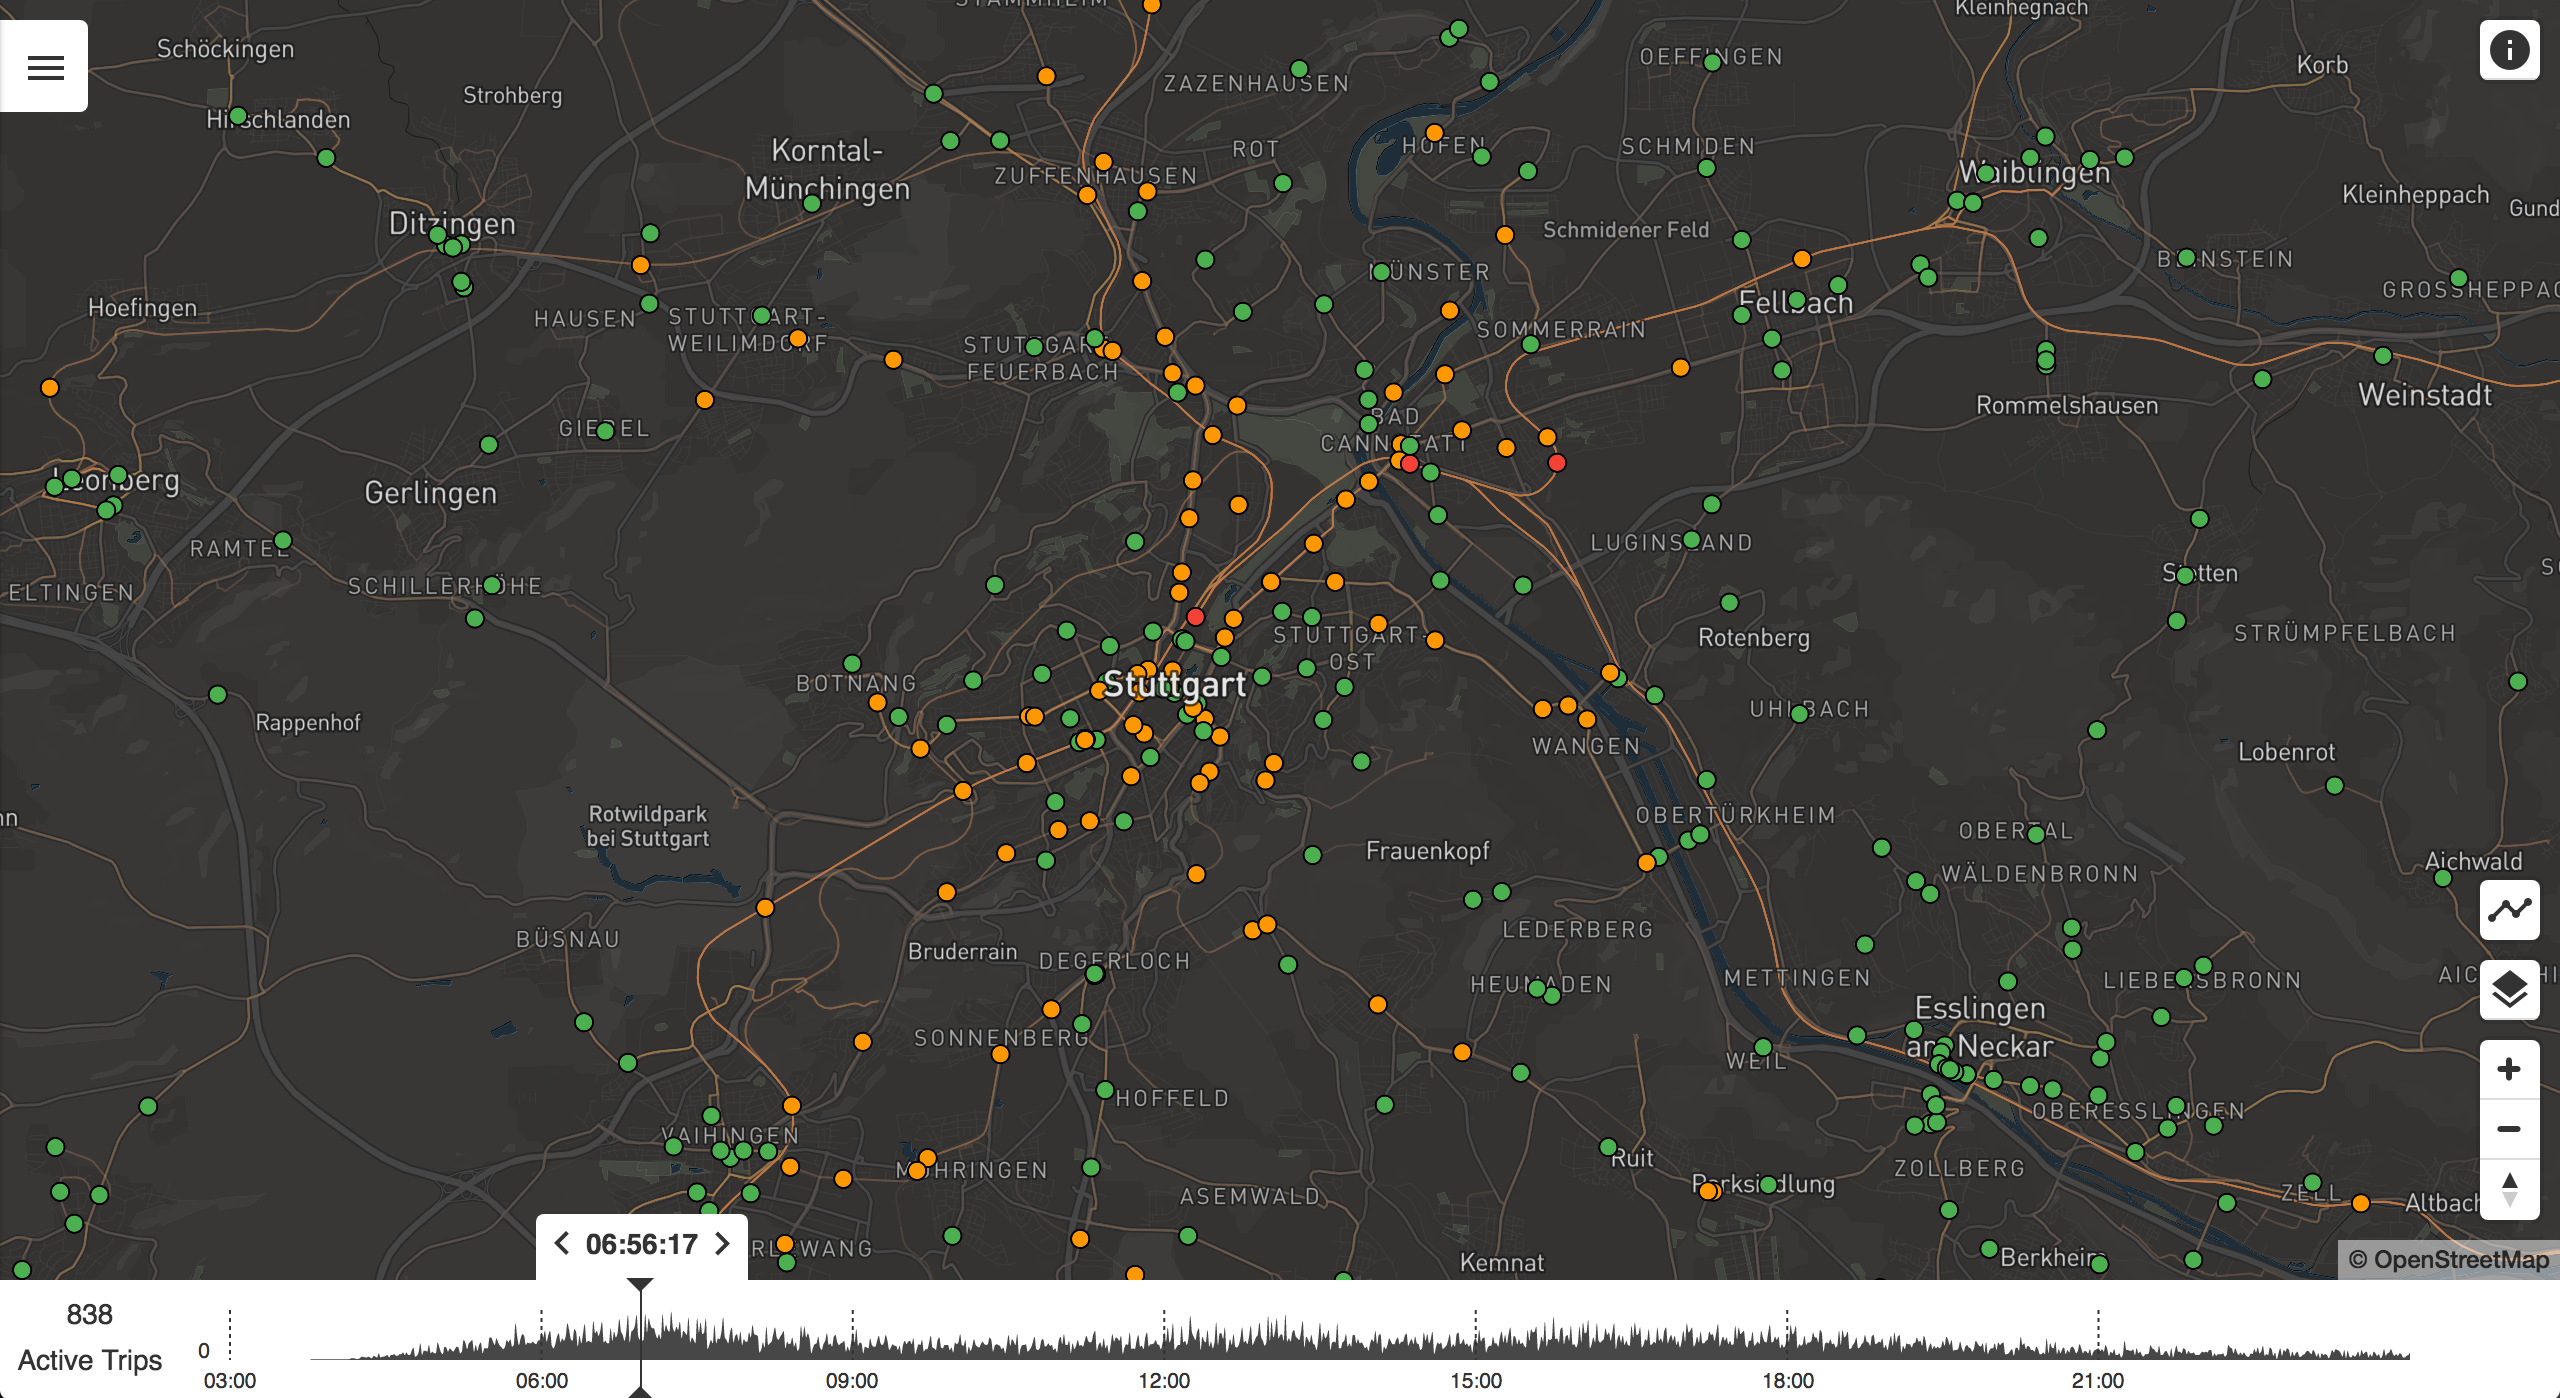
\includegraphics[width=0.99\textwidth]{rtt-map}
            \caption{Screenshot der fertigen Webanwendung}
            \label{fig:rtt-map}
        \end{center}
    \end{figure}
    
% subsection hinführung_zum_thema (end)
		\subsection{Gliederung der Arbeit}
\label{sub:gliederung_der_arbeit}
  Das Projekt wurde nach dem Design-Prinzip \texttt{"`The Double Diamond"'}\footnote{\url{http://www.designcouncil.org.uk/news-opinion/design-process-what-double-diamond}} bearbeitet, welcher der vorliegenden schriftlichen Ausarbeitung auch als Gliederungsgrundlage dient. Der Double Diamond wurde vom British Design Council 2005 entwickelt und soll im Folgenden kurz beschrieben werden.\parencite{designcouncil}

  \begin{figure}[htbp]
    \begin{center}
      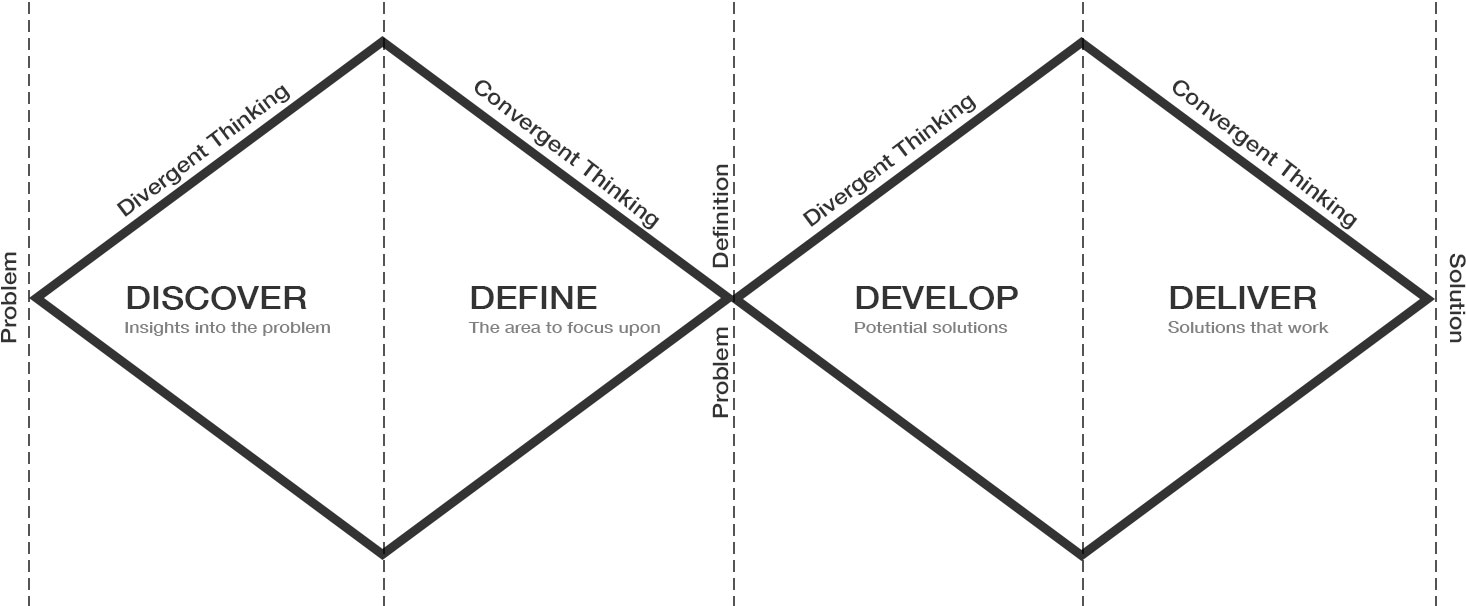
\includegraphics[width=0.9\textwidth]{double_diamond}
      \caption{"`The Double Diamond"' eigene Abbildung nach \parencite{designcouncil}}
      \label{fig:double_diamond}
    \end{center}
  \end{figure}

  Der Double Diamond beschreibt einen iterativen Prozess. Wie in allen kreativen Prozessen werden dabei eine Reihe von möglichen Ideen geschaffen ("divergentes Denken"), bevor sie verfeinert und auf die beste Idee reduziert werden ("konvergentes Denken"). Der Double Diamond zeigt jedoch an, dass dies zweimal geschieht - einmal zur Bestätigung der Problemdefinition und einmal zur Erstellung der Problemlösung. Einer der größten Fehler wäre es, den linken Diamanten und damit auch die Zieldimension zu vernachlässigen und am Ende womöglich das falsche Problem zu lösen.

  \begin{itemize}[label={}]
    \item \textbf{Discover:} Der erste Teil des Double Diamond steht am Anfang des Projektes. Hier wird versucht, die Welt neu zu sehen, Neues wahrzunehmen und Einsichten in das zu lösende Problem zu sammeln.

    \item \textbf{Define:} Der zweite Teil stellt die Definitionsphase dar. Dabei wird versucht, alle in der Entdeckungsphase identifizierten Möglichkeiten zu verstehen. Ziel ist es, ein klares Briefing zu entwickeln, das die grundsätzlichen Herausforderungen umreißt.

    \item \textbf{Develop:} Der dritte Teil markiert eine Entwicklungsphase, in der Lösungen oder Konzepte erstellt, prototypisiert, getestet und iteriert werden. Dieser Prozess des Ausprobierens hilft, Ideen zu verbessern und zu verfeinern.

    \item \textbf{Deliver:} Der letzte Teil des Double Diamond ist die Lieferphase, in der das daraus resultierende Projekt (z. B. ein Produkt, eine Dienstleistung oder eine Umwelt) abgeschlossen, produziert und in Betrieb genommen wird.

  Auf den Aufbau dieser Arbeit bezogen, werden diese Phasen auch für die Bezeichnung der Kapitel verwendet, in denen der Entwicklungsprozess der Webanwendung beschrieben wird. 

  \end{itemize}

% sub:gliederung_der_arbeit (end)

		% Aufzählen der eigenen Features der Karte. Was für Sachen wurden entworfen etc.

		% Aufzählen was in den einzelnen Kapiteln noch alles behandelt wird.

\end{newpage}

  \begin{newpage}
  \section{Discover}
  \label{sec:discover}
    In der Discover Phase soll der Blickwinkel möglichst weit geöffnet sein. 
    Dafür erfolgte eine weitreichende Recherche zu relevanten Themenbereichen wie Live Visualisierung, Visualisierung von öffentlichem Nahverkehr sowie Tools zum Erstellen von Karten (Abbildung \ref{fig:viz_overview}). 

    \subsection{Visualisierungsmöglichkeiten und Zielgruppe}
\label{sub:visualisierungsmöglichkeiten_und_zielgruppe}
  \begin{figure}[ht]
    \begin{center}
      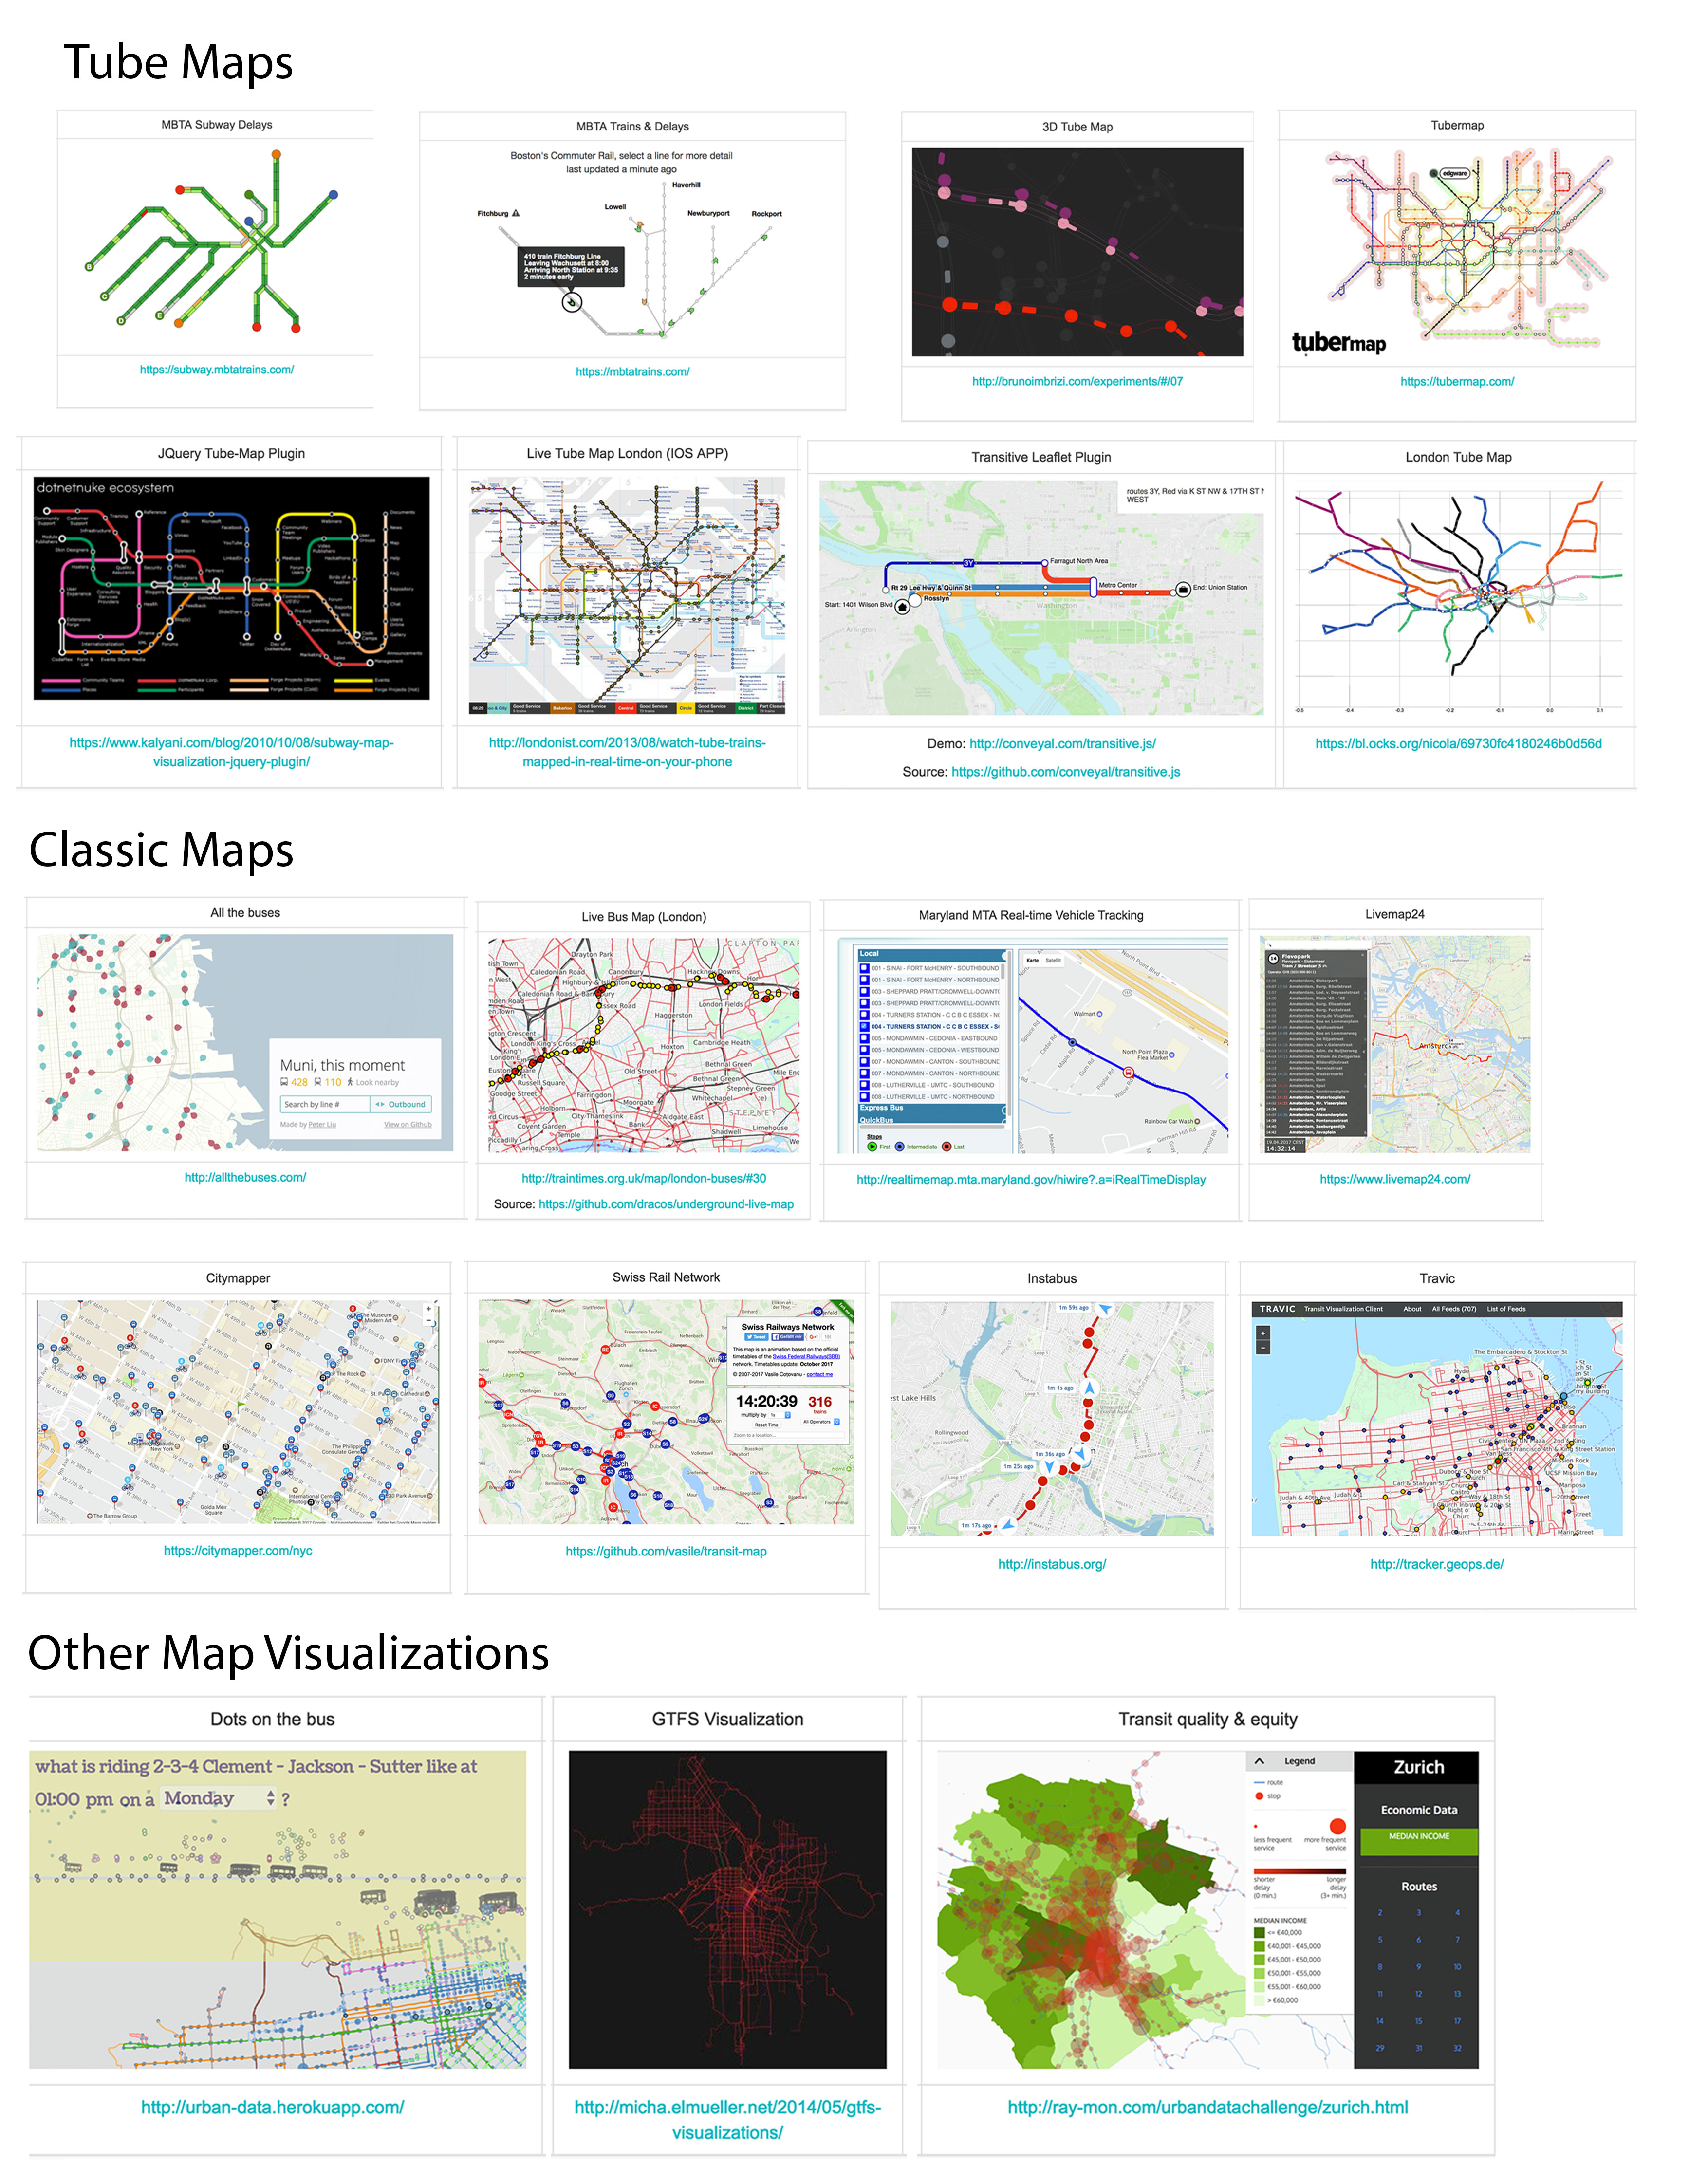
\includegraphics[width=0.8\textwidth]{viz_overview}
      \caption{Überblick über bestehende Tools und Visualisierungen}
      \label{fig:viz_overview}
    \end{center}
  \end{figure}

  Das gesammelte Material wurde in einer 2x2 Matrix (Abbildung \ref{fig:2x2_matrix}) in die Unterkategorien "`Live Map, Künstlerische Visualisierung, Plugin / Software / Tool, Tube-Map"' eingeordnet um einen sortierten Gesamtüberblick zu bekommen. 

  \begin{figure}[htbp]
    \begin{center}
      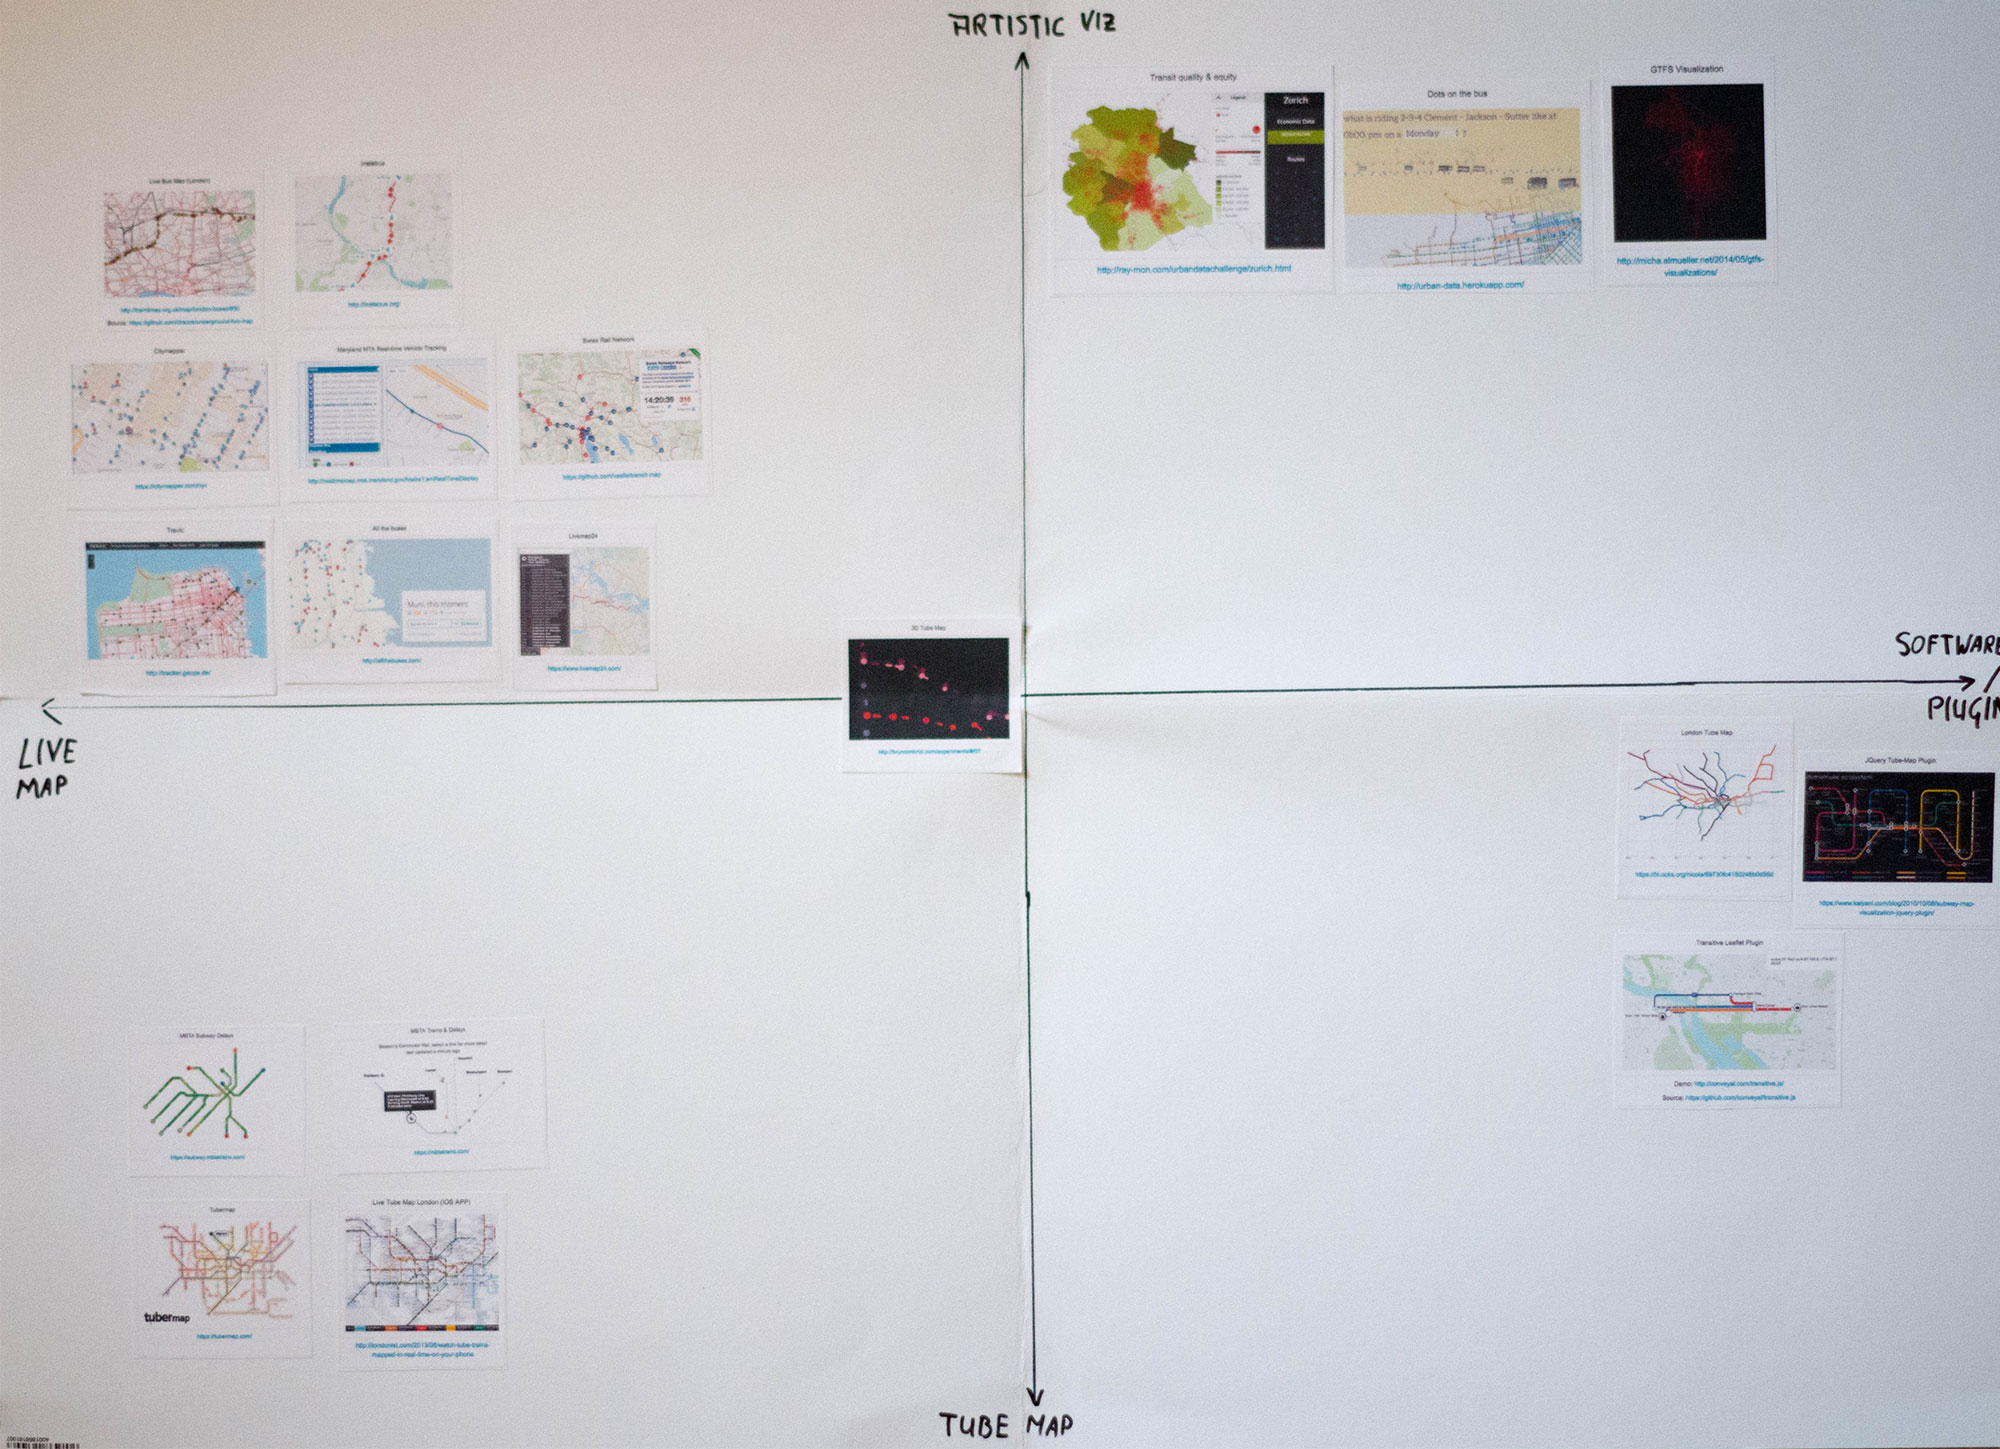
\includegraphics[width=0.5\textwidth]{2x2_matrix}
      \caption{2x2 Matrik Methode auf DIN A2}
      \label{fig:2x2_matrix}
    \end{center}
  \end{figure}

  Durch diese Ansicht wurde die Erkenntnis gewonnen, dass es schon viele Live Visualisierungen auf interaktiven Karten gibt, aber nur sehr wenig so genannten Tube-Maps. Auch sind bereits verschiedenste Tools zum generieren von GTFS basierten Visualisierungen vorhanden. Eine sehr ausführliche, aber bei weitem nicht vollständige, Liste über das Thema "`Transit"' wurde auf Github von der Community zusammengetragen \url{https://github.com/luqmaan/awesome-transit}.
% subsection visualisierungsmöglichkeiten_und_zielgruppe (end)

    
  % section discover (end)
\end{newpage}

  \section{Define}
\label{sec:define}
  Während in der \texttt{Discover-Phase} nur Ideen gesammelt und aufgelistet wurden, soll in diesem Kapitel die \texttt{Define-Phase} betrachtet werden. Dabei geht es darum, die getroffenen Entscheidungen zu begründen und zu konkretisieren als auch die begrifflichen Grundlagen dieser Arbeit zu definieren.
  
  \subsection{Kartenart}
\label{ssub:kartenart}
  Aus der Discover-Phase sind verschiedene Ideen bezüglich der Darstellungsarten entstanden. Zum Beispiel sah eine mögliche Lösung vor, die interaktive Karte mit anderen Visualisierungsformen zu kombinieren. So könnten die einzelnen Trips auch als Balkendiagramm dargestellt werden, welches den Fortschritt der zurückzulegenden Strecke verbildlicht. Dabei war angedacht, dass zwischen diesen verschiedenen Visualisierungsformen hin- und hergeschalten werden kann. Auch der Ansatz, dies mit einer Tube-Map zu verbinden, wurde als Idee notiert und war zeitweise als mögliches Ziel definiert. Da sich für Tube-Maps allerdings keine Kartenanbieter fanden, konnte diese Kartenart nicht umgesetzt werden.
  Letztendlich wird angestrebt, eine Classic-Map zu entwerfen, bei welcher die optische Karte subtil gestaltet ist, sodass die animierten Vehicle im Vordergrund stehen. Darüber hinaus sollen dem Anwender einige Standardfunkionen wie Zooming oder Panning zur Interaktion bereitgestellt werden.
  Es wurde entschieden, bei der Entwicklung der Live-Karte zunächst keine spezifische Nutzergruppe anzuvisieren, sondern einen möglichst universellen Prototypen zu entwerfen, welcher vielseitig genutzt und in unterschiedliche Richtungen weiterentwickelt werden könnte.  

% subsubsection kartenart (end)
  \subsection{Wahl der Datengrundlage}
\label{ssub:wahl_der_datengrundlage}
  Im Abschnitt "`\nameref{ssub:einsatz_von_gps_daten}"' wurde bereits erklärt, wie der Einsatz von GPS-Daten eine Live Visualisierung ermöglichen könnte. Der Einstaz von GPS hat aber allerlei schwachstellen, die auf den ersten Blick vielleicht nicht offensichtlich sind.

  \begin{itemize}[label={}]
    \item \textbf{Fehlende Datenverfügbarkeit:}
      Ein Weg, um Echtzeitdaten zu visualisieren, wäre die Verarbeitung von GPS Daten, die von den jeweiligen Verkehrsverbünden zur Verfügung gestellt werden müssten. Dies ist allerdings nicht der Fall. Zwar gibt es durchaus eine Erfassung der öffentlichen Verkehrsmittel, allerdings werden diese nicht für Dritte zur Verfügung gestellt. Die HaCon GmbH sammelt beispielsweise solche Daten, indem sie diese durch in den Fahrzeugen integrierte Software berechnet.\parencite{havasBusradar}. Es wären also GPS Daten vorhanden, da sie unter anderem im Bus-Radar der Deutschen Bahn (entwickelt von HaCon) verwendet werden, sie sind allerdings weder über eine API noch anderweitig für die Öffentlichkeit erhältlich. Über die rechtlichen Belange und ob solche Daten in Deutschland überhaupt öffentlich gemacht werden dürften, soll an dieser Stelle nicht diskutiert werden\footnote{In \textit{"`Opening Public Transit Data in Germany"'} von Stefan Kaufmann\parencite{kaufmann} wird dieses Thema der Rechtslage näher betrachtet.}.

    \item \textbf{Aktualisierungsintervall:}
      Abseits der fehlenden Beschaffung von GPS Daten haben diese noch einen weiteren Nachteil. Vehicle, die mit einer GPS Lokalisierung ausgestattet sind, senden keinen kontinuierlichen Strom an Daten, sondern nur in einem gewissen Aktualisierungsintervall. Zwar preist HaCon seinen Busradar durch folgende Aussage an: 

      \begin{quote}
        \textit{"`Der neue Busradar eignet sich hervorragend, um die eigene Fahrt zu visualisieren und Anschlussfahrzeuge zu verfolgen. Erstmals geschieht dies GPS-basiert und nicht durch interpolierte Echtzeitdaten, was eine noch höhere Genauigkeit zur Folge hat."'}\parencite{havasBusradar}
      \end{quote}

      Nähme man aber nur die GPS Daten als Basis für eine Visualisierung, so würde der Bus bei jeder Aktualisierung von der jeweils vorherigen Position zur nächsten springen. Dieses "`Springen"' kann beim Busradar dann auch dazu führen, dass der Nutzer einen Bus auf seiner App verfolgen will, aber dieser nach dem nächsten GPS Update nicht mehr auf dem Display zu sehen ist, da er nun außerhalb des Viewports liegt. Dieses Verhalten kann den Nutzer durchaus verwirren, da nicht klar ist, in welche Richtung sich das Vehicle bewegt hat, sodass in alle Richtung gesucht werden muss.

    \item \textbf{Verlässlichkeit \& Verfügbarkeit:} 
      Zudem sind GPS Signale nicht immer verlässlich. Sie können oftmals gestört werden oder die Verbindung zum Satelliten verlieren. Wie würde sich in einem solchen Fall des Signalverlusts die Live Visualisierung verhalten? Verschwindet das Vehicle von der Karte oder bleibt es für längere Zeit auf der Stelle stehen? Beide Möglichkeiten erscheinen als nicht optimal. 

      Zuletzt sei erwähnt, dass ein GPS basiertes System für U- und S-Bahn erst gar nicht infrage käme, da diese unterirdisch verlaufen und andere Technologien für deren Erfassung eingesetzt werden müssten. Für eine Live Karte, die nicht nur Busse, sondern auch andere Verkehrsmittel abbilden möchte, ist die GPS basierte Lokalisierung folglich nicht zielführend.
  \end{itemize} 

  Wie zu sehen ist sind diese Probleme nicht unerheblich. Vor allem das fehlen der Daten, macht eine GPS basierte Visualisierung unmöglich.\\

  Aber auch GTFS besitzt Nachteile. Für eine Live Visualisierung fehlt ihr die Echtzeitkomponente. Die Fahrplandaten stellen nur einen \texttt{Soll-Zustand} dar, der erheblich vom \texttt{Ist-Zustand} abweichen kann. Auch die Geschwindigkeit eines Vehicles entspricht bei einer Interpolation der Durchschnittsgeschwindigkeit, die sich Anhand der Fahrplandaten ausrechnen lassen. Benötigt ein Vehicle $V$ von Station A nach B 3 Minuten für eine Strecke von 1.2 Kilometer, so würde die Animation eine durchschnittliche Geschwindigkeit von $v = \frac{s}{t} = \frac{1.2 \: \cdot \: 1000}{3 \: \cdot \: 60} = 6.6 \: \frac{m}{s} = 23.76 \: \frac{km}{h}$ errechnen.

  % TODO: sowas wie: "die Interpolation wird noch ausführlicher in Kapitel xy behandelt"

  Eine genauere Erfassung der Geschwindigkeit wäre zwar Wünschenswert, bringt allerdings andere Schwierigkeiten mit sich. Die Erfassung der Geschwindigkeit von jedem Vehicle würde eine hohe Menge an Daten bedeuten, die zwischen Server und Client ausgetauscht werden müssen. Ähnlich wie bei einer GPS basierten Animation, wäre der Client komplett davon abhängig, ständig Daten zu erhalten. Stelle man sich vor das mehrere hundert Anwender eine App benutzen wäre dies eine enorme Menge an Anfragen \& Antworten. Für Smartphones mit schlechter Verbindung ist dieser Umstand ein großes Problem. Ebenso wie die verwendete Bandbreite und der erhöhte Batterieverbrauch durch das ständige Stellen von Anfragen und der Verarbeitung der Antwort.

  Die Vorteile ergibt sich aus den eben genannten Nachteilen. Bei einer Interpolation des Fahrplans, ist keine ständige Verbindung zum Server nötig. Existiert der relevante Teil des Fahrplans auf dem Gerät des Endnutzers, so kann die Animation anhand dieser Daten erfolgen. Zudem wird das Problem des "`springens"' Umgangen, welches vor allem bei GPS basierter Animation ein Problem darstellt. Durch die Interpolation sind glatte Animationen der Vehicle auf der Karte möglich. Durch die Bewegung des Vehicles von A nach B entspricht die Visualisierung mehr dem Verhalten von Fahrzeugen in der realen Welt. Dadurch kann der Anwender besser nachvollziehen was geschieht.
  Eine Lösung für das Problem der fehlenden Echtzeiterfassung ließe sich GTFS-Realtime einsetzen. In dieser Arbeit kann GTFS-realtime allerdings nicht zum Einsatz kommen, da zum jetzigen Zeitpunkt\footnote{September, 2017}, der Verkehrsverbund Stuttgart-VVS dies nicht (auch nicht durch ein anderes Format) öffentlich anbietet.
  
% subsubsection wahl_der_datengrundlage (end)
  \subsection{Gewählte Technologien}
\label{ssub:gewählte_technologien}
  Die auszuwählenden Technologien für ein solches Projekt sind zahlreich. Da es sich bei dieser Arbeit um keine Produktentwicklung mit eingeschränktem Nutzerkreis handelt, besteht bei der Technologieauswahl uneingeschränkte Freiheit. Um diesen Umstand auszunutzen und dem Projekt einen experimentellen Charakter zu verleihen, sollen vor allem zukunftsweisende Technologien Verwendung finden.
  
  \subsubsection{Datenbank}
  \label{ssub:datenbank}
    Da der GTFS Standard eine fertige relationale Beziehung der einzelnen Dateien festlegt, ist der Einsatz einer relationalen Datenbank sehr naheliegend. Dabei gibt es eine breite Palette an Auswahl. Damit die Anwendung möglichst zugänglich bleibt, liegt der Fokus auf Datenbanken, die unter einer Open-source-Lizenz kostenfrei zur Verfügung stehen. Die zwei populärsten sind MySQL und PostgreSQL\parencite{db_engines}. Beide haben ihre Vor- und Nachteile und die Entscheidung ist mehr eine persönliche Präferenz, als ein großer Vorteil des Einen über den Anderen. Einen kleinen Vorteil bietet PostgreSQL's Unterstützung für Array-Types, welche sehr hilfreich beim Speichern und Abfragen von Daten ist. So fiel die Entscheidung auf die PostgreSQL Datenbank, wobei eine Realisierung auch mit MySQL möglich gewesen wäre.
  % subsubsection datenbank (end)

  \subsubsection{Serverwahl}
  \label{ssub:serverwahl}
    Für das Backend soll \texttt{Nodejs} verwendet werden. Nodejs ist nicht nur einfach aufzusetzen, sondern auch sehr performant und effizient für Web Applikationen einsetzbar. Zudem lässt es sich sehr einfach mittels Docker in der AWS (Amazon Web Services) Cloud veröffentlichen. Da Nodejs dynamisch typisiert, lassen sich vor allem auch Prototypen sehr schnell erstellen. Zusätzlich können sowohl Server und Client in JavaScript programmiert werden, wodurch die meisten Frameworks sowohl für den Server als auch für den Client zur Verfügung stehen.
  % subsubsection serverwahl (end)
  
  \subsubsection{Kartenmaterial}
  \label{ssub:kartenmaterial}
    Bereits zu Beginn wurde von einer hohen zu bewältigenden Datenmenge ausgegangen. Um die Voraussetzungen dafür zu schaffen, wurde nach Softwarelösungen gesucht, die für solche Datenmengen ausgelegt sind. Für die Karte wird dafür Mapbox eingesetzt. Mapbox verwendet Web-GL (basierend auf OpenGL) und bietet damit die Möglichkeit, ein GPU unterstütztes Rendering im Browser zu ermöglichen. Zusätzlich bietet Mapbox gegenüber Google-Maps den Vorteil von eigene Karten-Styles. Diese können über Mapbox-Studio voll umfänglich auf die eigenen Bedürfnisse angepasst werden. Parks, Straßen, Schriftzüge, nahezu alle Elemente der Karte, lassen sich ändern und anpassen. Zusätzlich können eigene Daten in die Karte integrieren werden, was Bandbreite und Rechenleistung spart. Damit konnten sämtliche Routen, die das Stuttgart-VVS Feed beinhaltet, in das Kartenmaterial gezeichnet werden (siehe orangene Linien in Abbildung \ref{fig:map_tiles_routes}).

    \begin{figure}[htbp]
      \begin{center}
        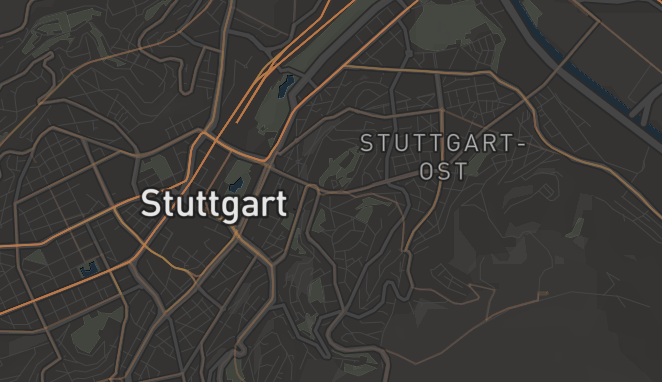
\includegraphics[width=0.5\textwidth]{map_tiles_routes}
        \caption{Karte mit integrierten Stuttgart-VVS Daten}
        \label{fig:map_tiles_routes}
      \end{center}
    \end{figure}
    
    Die Wahl der richtigen Tools ist dabei nur die Grundlage, um die Datenmenge zu bewältigenden. Viele weitere Schritte sind notwendig, um eine performante Webanwendung zu erstellen und werden in im nächsten Kapitel \nameref{sec:develop} noch ausführlicher aufgeführt.
    
  % subsubsection kartenmaterial (end)

  \subsubsection{Frameworks}
  \label{ssub:frameworks}
    Für die Programmierung wurden folgende Bibliotheken ausgewählt. Diese bieten verschiedenste Erleichterungen bei der Programmierung.

    \begin{itemize}[label={}]
      \item \textbf{Turf}\footnote{\url{http://turfjs.org/docs/}} stellt eine ganze Reihe an Funktionen für die raumbezogene Verarbeitung von Daten zur Verfügung. Beispielsweise lassen sich mittels Turf unter anderem Distanzen, Flächen oder Schnittpunkte berechnen.

      \item \textbf{Mapbox-gl-js}\footnote{\url{https://www.mapbox.com/mapbox-gl-js/api/}} wird benötigt, um das Kartenmaterial von Mapbox im Client zu verwenden. Dafür stellt es eine eigene API zur Verfügung.

      \item \textbf{Lodash}\footnote{\url{https://lodash.com/}} ist eine Hilfsbibliothek, die verschiedene Funktionen zur Verfügung stellt, die das Arbeiten mit JavaScript vereinfachen.

      \item \textbf{Express}\footnote{\url{https://expressjs.com/en/starter/basic-routing.html}} ist ein minimalistisches Node.js Framework für moderne Web-Applikationen. Es vereinfacht die Erstellung von API Endpunkten durch das Bereitstellen hilfreicher Methoden zur Erstellung des Routing. Routing bezieht sich dabei auf die Bestimmung, wie eine Anwendung auf eine Client-Anfrage an einen bestimmten Endpunkt reagiert, also auf eine URI (oder einen Pfad) und eine bestimmte HTTP-Request-Methode (GET, POST usw.).
    \end{itemize}
    
  % subsubsection frameworks (end)
% subsubsection gewählte_technologien (end)
  \subsection{Zielsetzung}
\label{sub:zielsetzung}
  
  Das Hauptziel der Arbeit besteht darin, eine interaktive Karte zu entwickeln, die den Öffentlichen Nahverkehr des Verkehrsverbunds Stuttgart-VVS auf einer Live-Karte visualisiert. Dafür soll ein Prototyp entwickelt werden, der für Demonstrationszwecke eingesetzt werden kann. Weitere visuelle Ziele sollen sich im Prozess durch das Erkunden verschiedener Lösungsansätze ergeben. \\

  Außerdem werden Ziele in Bezug auf die Performance der einzelnen Komponenten (Datenbank, Server, Client) gesetzt. Die Datenbank soll ein GTFS-Feed der Stuttgart-VVS aufnehmen und dessen Daten in $0$ bis $200ms$ bereitstellen können. Des Weiteren soll der Nodejs-Server die Daten innerhalb von maximal $100ms$ verarbeitet haben. Das Frontend soll die Vehicle mit 60 FPS rendern können.\\

  
% subsection zielsetzung (end)
  \subsection{Begriffe und Definitionen}
\label{sub:begriffe}
  Bevor im nächsten Kapitel "`\nameref{sec:develop}"' die Umsetzung des Projekts beschrieben wird, sollen zur Sicherstellung eines gemeinsamen Verständnisses zuerst die verwendeten Begrifflichkeiten geklärt bzw. definiert werden.

  \subsubsection{Time}
  \label{ssub:time}
    In verschiedenen Formeln wird immer wieder eine Time $t_{cur}$ referenziert. Diese beschreibt die globale (aktuelle) Zeit des Systems in Sekunden. 
    Die Sekunden lassen sich durch das Addieren der Stunden, Minuten und Sekunden errechnen.\\

    Bsp: 17:04:59 Uhr\\

    $t_{cur} = $ Stunden $*$ 3600 $+$ Minuten $*$ 60 $+$ Sekunden\\
    $\Rightarrow$ $t_{cur} = 17 * 3600 + 4 * 60 + 59 = 61499 \; sec$
    
  % subsubsection time (end)

  \subsubsection{Vehicle}
  \label{ssub:vehicle}
    Ein Vehicle $V$ beschreibt in dieser Arbeit ein Fahrzeug, welches im Dienste der öffentlichen Verkehrsbeförderung steht. Dies sind beispielsweise Bus, U- \& S-Bahn, Interrail Züge aber auch Zahnradbahn oder gar Funicular-Services\footnote{\url{https://en.wikipedia.org/wiki/Funicular}}. Das private Automobil fällt folglich nicht unter diese Definition.
  % subsubsection vehicle (end)

  \subsubsection{Polyline}
  \label{ssub:polyline}
    Eine Polyline\footnote{Linienverlauf bzw. auch Shape genannt} $P$ ist eine Kurve, die sich durch eine Sequenz an Punkten $\{ p_1, \dotsc, p_n \;|\; n \in \mathbb{N} \}$ definiert. Sie beschreibt den zurückzulegenden Verlauf eines Vehicles.
  % subsubsection polyline (end)

  \subsubsection{Station}
  \label{ssub:station}
    Eine Station $S$ ist eine Haltestelle, die von einem Vehicle $V$ während eines Trips $T$ angefahren wird und sich entlang einer Polyline befindet. Die Station definiert dabei die Ankunfts- und Abfahrtszeiten, wann ein Vehicle an dieser Station anhält und wann es diese zur Weiterfahrt wieder verlässt. Ankunfts- und Abfahrtszeit seien wie folgt definiert: \texttt{arrival time} $ := t_{ari}$ und \texttt{departure time} $ := t_{dep}$.

  \subsubsection{Trip}
  \label{ssub:trip}
    In dieser Arbeit wird immer wieder der Begriff "`Trip"' Verwendung finden. Ein Trip $T$ sei mit folgenden Eigenschaften definiert:
    \begin{itemize}
      \item $T$ besteht aus einer Anzahl an Stationen: $T = \{S_1, \dotsc, S_n \;|\; n \in \mathbb{N}, n \geq 2 \}$

      \item Ein Trip $T$ wird dabei von genau einem Vehicle $V$ bedient. Daraus folgt $T$ mit dem Mapping: $T \mapsto V$ ist Injektiv zu $V$. 

      \item Ein Trip $T$ besitzt genau eine Polyline $P$. $T \mapsto P$ $ \Rightarrow T$ ist injektiv zu $P$. 

      \item Die Bewältigung der Strecke $\{A,B \;|\; A, B \in S\}$ entlang einer Polyline $P$ durch ein Vehicle $V$ gilt als ein einziger Trip.

      \item Ein Trip beginnt genau dann, wenn die momentane Zeit $t_{cur}$ mit der Abfahrtszeit $t_{dep}$ der ersten Station übereinstimmt $\Rightarrow t_{cur} = t_{dep} $ .

      \item Ein Trip endet genau dann, wenn die momentane Zeit $t_{cur}$ mit der Ankunftszeit $t_{ari}$ der letzten Station übereinstimmt $\Rightarrow t_{cur} = t_{ari} $ .

      \item Der Rückweg $\{B, A \ni T \;|\; A, B \in S\}$ ist nicht in einem Trip $T$ enthalten, sondern wird als ein neuer Trip erfasst.
    \end{itemize}
    
  % subsubsection trip (end)

    \subsubsection{Route}
    \label{ssub:route}
      Eine Route $R$ besteht aus einer Anzahl an Trips $T \geq 1$. Eine Route vereint alle vorherigen Relationen in sich. Abbildung \ref{fig:gtfs_viz} veranschaulicht diese. 

      \begin{itemize}
        \item $R = \{ T_1, \dotsc, T_n \;|\; n \in \mathbb{N}, n \geq 1 \}$

        \item $R$ mit dem Mapping: $R \mapsto T$ ist surjektiv\footnote{Eine Route kann mehrere Trips besitzen, wohingegen ein Trip nur einer Route zugehörig sein kann.} 
      \end{itemize}     

      \begin{figure}[htbp]
        \begin{center}
          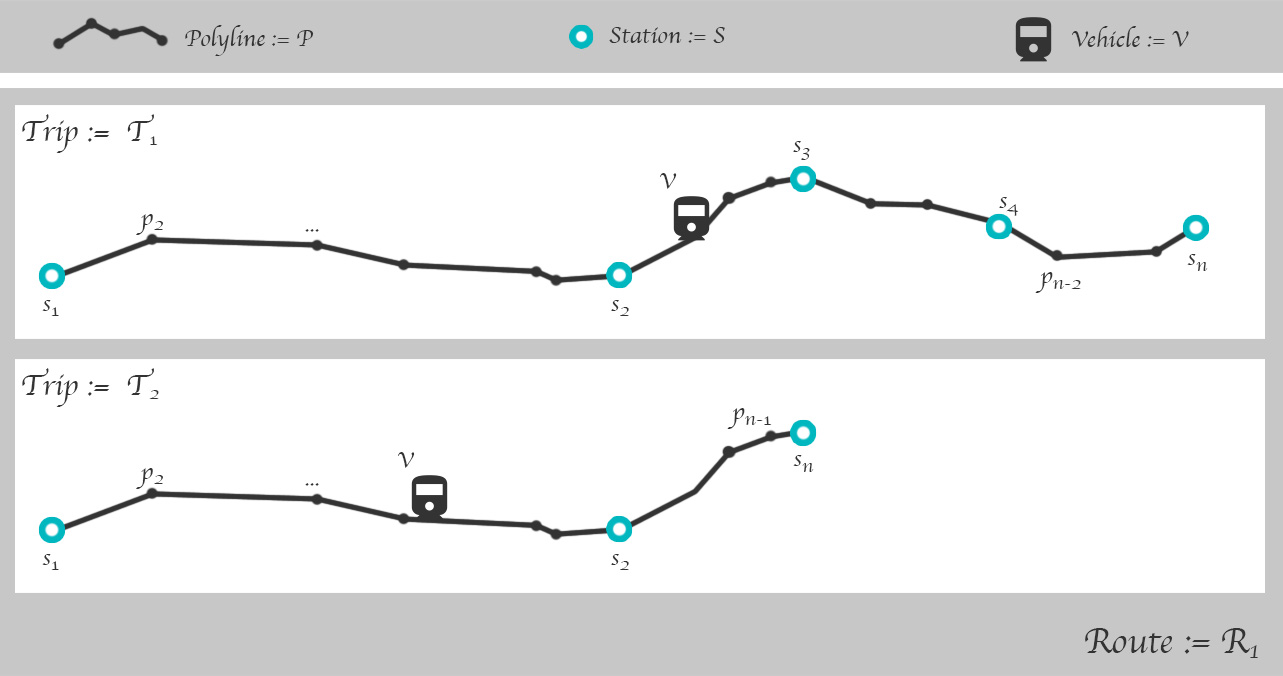
\includegraphics[width=\textwidth]{gtfs_viz.jpg}
          \caption{Grafische Veranschaulichung einer Route}
          \label{fig:gtfs_viz}
        \end{center}
      \end{figure}

      Abbildung \ref{fig:gtfs_viz} zeigt, dass eine Route zum Beispiel alle Trips einer U-Bahn-Linie erfasst. Eine U-Bahn-Linie muss dabei nicht immer an allen Stationen halten, sondern kann beispielsweise im Nachtbetrieb auch Stationen auslassen (zu sehen bei Trip $T_2$). Trotzdem werden nur diejenigen Trips in einer Route vereint, die dem selben Routenverlauf folgen.
    % subsubsection route (end)

% subsection begriffe (end)
  
% section define (end)

  \begin{newpage}
  \section{Develop}
  \label{sec:develop}
    % TODO: AWS - Instanz spezifikationen (Leistung) Medium Instanz?
    % TODO: AWS - Server Test bzw Metriken?

    In diesem Kapitel wird der Entwicklungsprozess dargestellt. In diesem Dokument ist dieser Prozess sehr linear beschrieben wohingegen der eigentliche Ablauf nicht immer dieser Linearität entsprach. Zuerst soll beschrieben werden, was getan werden musste um ein einzelnes Vehicle entlang einer Polyline zu animieren. Anschließend wird dieser Ansatz weiterentwickelt, bis die Animation von allen aktiven Trips auf einer Karte möglich sind. Dabei werden verschiedene Optimierungsmaßnahmen ergriffen, um Probleme bezüglich der Performance zu beseitigen. Vor allem die zu verarbeitende Datenmenge, als auch das verarbeiten und optimieren von GTFS Feeds, sind die Kernpunkte in diesem Kapitel. 

    \subsection{Anzeigen einer Polyline}
\label{sub:anzeigen_einer_polyline}
  Zu Beginn stellte sich die Frage, wie sich in kleinen Schritten an das komplexe Thema einer Live-Visualisierung herangetastet werden kann. Die erste Hürde ist die Animation von nur \textbf{einem} Vehicle entlang einer Polyline. Die Umsetzung dieses ersten Schrittes soll in diesem und den nächsten zwei Abschnitten \ref{sub:hinzufügen_der_stationen} und \ref{sub:animieren_eines_vehicles_durch_interpolation} erklärt werden.

  Um eine Datengrundlage zu haben, wurde ein möglichst vollständiges GTFS-Feed  ausgewählt\footnote{\url{http://TransitFeeds.com}} und in die Datenbank importiert. Die Wahl fiel dabei auf das Boston-MBTA Feed. Die Herausforderung bestand nun darin, erste Daten aus der Datenbank an den Client zu senden und sie dort darzustellen. Fast trivial ist das Abfragen der Polyline:

  \colorbox{lightGrey}{\texttt{\color{white}{{\color{materialBlue} SELECT} * {\color{materialBlue}FROM} gtfs\_shapes {\color{materialBlue}WHERE} shape\_id = {\color{materialRed}12345}}}}

  \begin{figure}[htbp]
    \begin{center}
      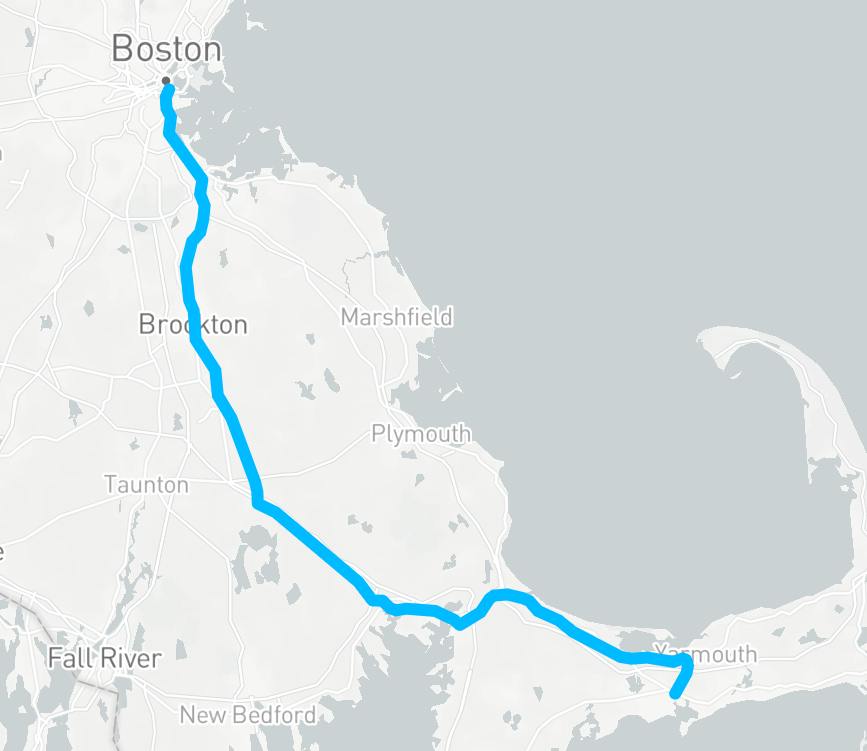
\includegraphics[width=0.5\textwidth]{prozess/draw_single_shape}
      \caption{Anzeigen einer einzigen Polyline in Boston}
      \label{fig:prozess/draw_single_shape}
    \end{center}
  \end{figure}
  
  Die Daten der Polyline werden als GeoJSON übertragen und lassen sich mittels Mapbox-gl-js auf der Karte anzeigen. Abbildung \ref{fig:prozess/draw_single_shape} zeigt das Ergebnis dieser ersten Iteration. Zu sehen ist bereits die Karte mit der Polyline (hier in blau). Die abgefragten Daten können nun also bereits verarbeitet und angezeigt werden. Damit ein Vehicle entlang dieser Linie animiert werden kann, werden die einzelnen Stationen des Trips benötigt.
  Dieser ständige Wechsel zwischen der Arbeit am Backend, um neue Datenabfragen zu ermöglichen und dem Frontend, um diese anschließend anzuzeigen, stellte sich als sehr effektiv heraus und zog sich durch das gesamte Projekt hinweg durch.
% subsection anzeigen_einer_polyline (end)
    \subsection{Hinzufügen der Stationen}
\label{sub:hinzufügen_der_stationen}
  Nachdem die Polyline auf die Karte gebracht wurde, werden die Stationen des Trips benötigt (Abbildung \ref{fig:prozess/add_stations}). Diese beinhalten für die Animation essentielle Daten wie zum Beispiel Abfahrts- und Ankunftszeit eines Vehicles. Die genaue SQL-Abfrage dafür soll an dieser Stelle der Einfachheit wegen ausgespart bleiben.

  \begin{figure}[htbp]
    \begin{center}
      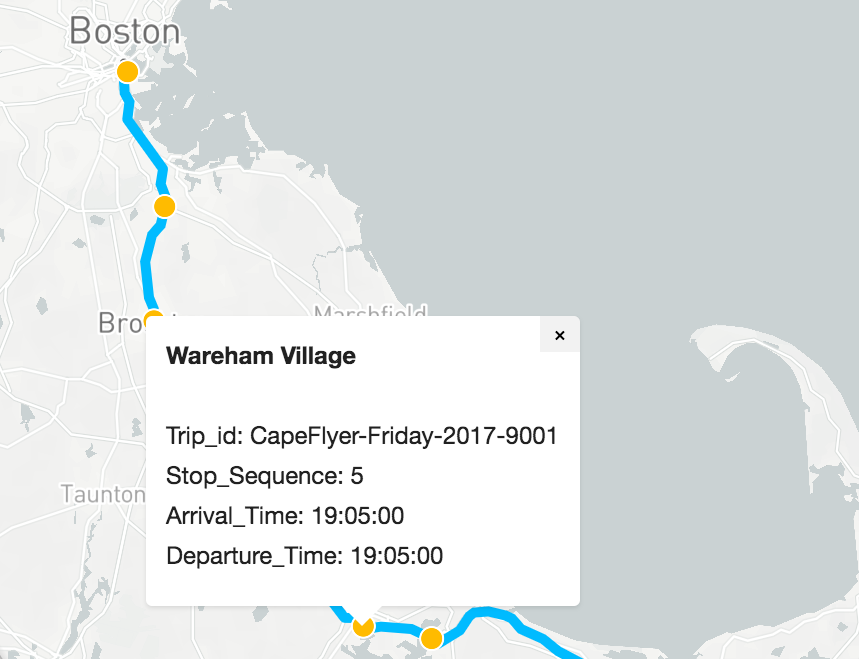
\includegraphics[width=0.5\textwidth]{prozess/add_stations}
      \caption{Hinzufügen von Stationen entlang der Polyline}
      \label{fig:prozess/add_stations}
    \end{center}
  \end{figure}

  Für die Animation der Vehicle (Abschnitt \ref{sub:animieren_eines_vehicles_durch_interpolation}) wird außerdem der Wert für die Differenz der \texttt{distance\_traveled}, also die Distanz zwischen den einzelnen Stationen, benötigt. Diese kann aus den distance\_traveled-Werten der einzelnen Stationen über Subtraktion berechnet werden. Nun hat zwar das Stuttgart-VVS-Feed ein distance\_traveled-Feld, welches die benötigten Distanz-Informationen direkt aus der Datenbank liefert; für andere GTFS-Feeds, die getestet wurden, ist dieses Feld jedoch oftmals nicht vorhanden. Aus diesem Grund wurde ein Algorithmus entwickelt, welcher über ein sogenanntes \texttt{Station-Matching} die Werte der distance\_traveled und damit die Distanz zwischen den Stationen ermitteln kann. Der Station-Matching-Algorithmus wird von der Applikation nur dann als Fallback-Lösung für die Berechnung verwendet, wenn das distance\_traveled-Feld nicht im Feed vorhanden ist.

  \subsubsection*{Station-Matching}
  \label{ssub:station_matching}
    Das Station-Matching soll folgendes Problem lösen:

    \begin{figure}[htbp]
      \begin{center}
        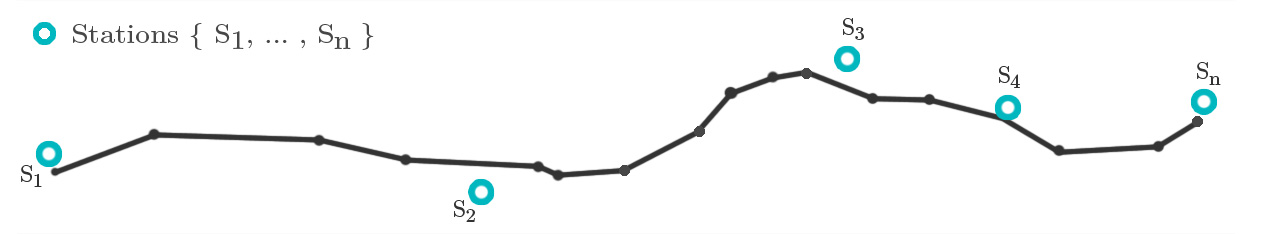
\includegraphics[width=\textwidth]{station_problem.jpg}
        \caption{Stationen liegen nicht direkt auf der Polyline}
        \label{fig:station_problem}
      \end{center}
    \end{figure}
    
    Wie in Abbildung \ref{fig:station_problem} zu sehen ist, sind die Stationen (Haltestellen oder Bahnhöfe) nicht exakt auf der Polyline, sondern ein wenig abseits positioniert, da dies auch ihrem realen Standort neben der Fahrbahn entspricht. Um nun die Distanzen zwischen den Stationen zu berechnen, legt der Algorithmus im Sinne des Matchings zunächst die Stationen auf die Polyline.  

    \begin{figure}[htbp]
      \begin{center}
        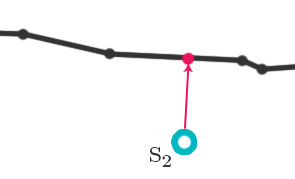
\includegraphics[width=0.25\textwidth]{find_nearest_point}
        \caption{Finde den nächstgelegenen Punkt der Station auf der Polyline}
        \label{fig:find_nearest_point}
      \end{center}
    \end{figure}

    Nachdem der entsprechende Punkt auf der Polyline gefunden wurde, berechnet der Algorithmus die jeweiligen Wegstrecken zur ersten Station des Trips (distance\_traveled), bevor er die Werte von aufeinanderfolgenden Stationen subtrahiert.  Die Distanz zweier Stationen $\{S_i,S_{i+1} \;|\; i \in \mathbb{N} \}$ sei $d_\triangle$. Diese kann jetzt wie folgt berechnet werden: $d_{\triangle_i} = d_{S_n} - d_{S_{n-1}}\;|\; d_S := DistanceTraveled, n \in \mathbb{N}, n \ge 2$ 
    In Listing \ref{lst:match_station} des Anhangs wird dieser Station-Matching-Algorithmus vorgestellt.

    \begin{figure}[htbp]
      \begin{center}
        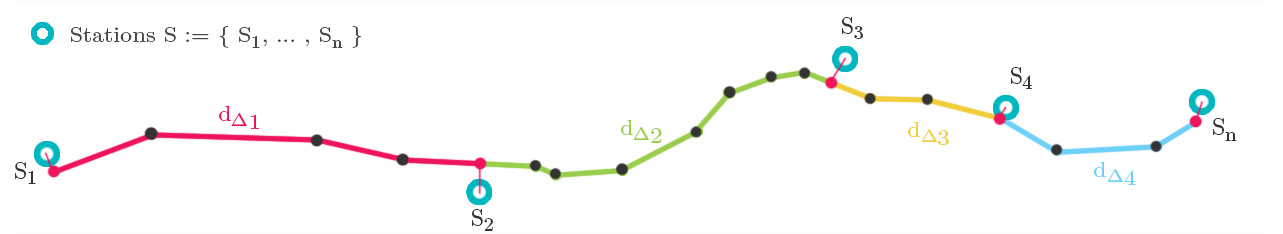
\includegraphics[width=\textwidth]{get_distances}
        \caption{Berechnen der Distanz}
        \label{fig:get_distances}
      \end{center}
    \end{figure}
    
    Abbildung \ref{fig:station_matching_comparision} stellt eine frühere Implementierung mit der nun aktuellen Version des Algorithmus gegenüber, indem die für das Matching über $n$-Trips benötigte Zeit der beiden Algorithmen verglichen wird. Um eine durchschnittliche Laufzeit zu erhalten, wurde jeder Algorithmus 10 mal mit der gleichen Anzahl an Trips ausgeführt.

    \begin{figure}[htbp]
      \begin{center}
        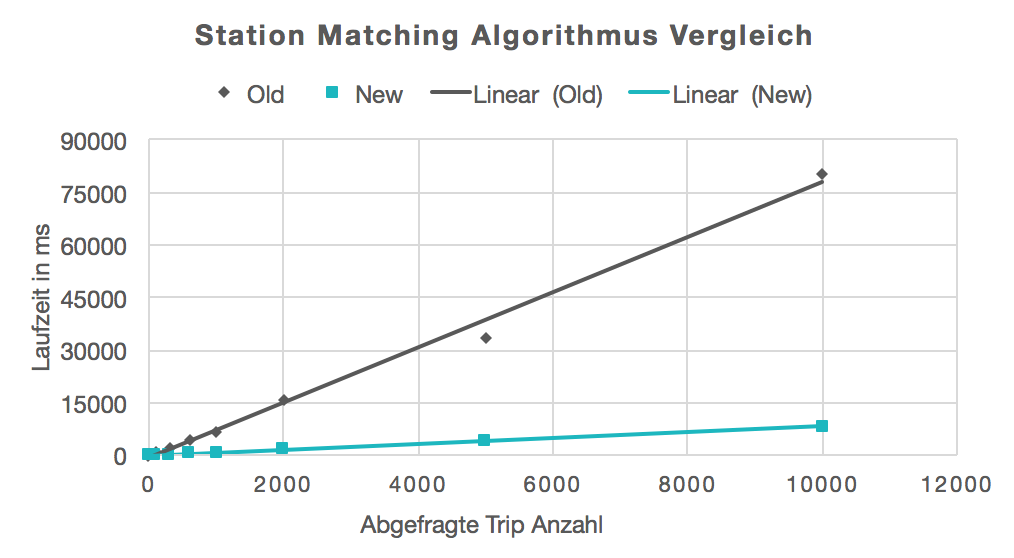
\includegraphics[width=0.7\textwidth]{station_matching_comparision}
        \caption{Vergleich der zwei Station-Matching-Algorithmen}
        \label{fig:station_matching_comparision}
      \end{center}
    \end{figure}

    Der alte Algorithmus war sehr simpel und beruhte darauf, die Funktion \texttt{pointOnLine} der \texttt{Turf.js}-Bibliothek zu verwenden. Diese Funktion hatte den entscheidenden Nachteil, dass sie in 3 \texttt{for}-Schleifen über die gesamten Punkte der Polyline iteriert. Hinzu kommt, dass das Matching nicht nur auf eine Station, sondern auf sämtliche Stationen aus allen Trips angewendet werden muss. Das führte dazu, dass insgesamt 5 \texttt{for}-Schleifen verwendet wurden. Damit lässt sich der im Vergleich höhere Anstieg der Laufzeit bei steigender Trip-Anzahl erklären. Generell ist der neue Algorithmus sehr viel schneller. Durch die Verwendung eines \texttt{R-Trees}\footnote{Ein R-Tree (R für Rectangle) bezeichnet eine baumförmige Datenstruktur für das Speichern und Abfragen von raumbezogenen Informationen. In Verwendung ist folgende Bibliothek: \url{https://github.com/mourner/rbush}} und der eigenen Implementierung verschiedener Bibliotheksfunktionen (turf.lineSlice, turf.pointOnLine), konnte die Laufzeit drastisch reduziert werden (siehe Tabelle \ref{tbl:station_matching_comparison}).

    \begin{longtable}{|>{\raggedright \arraybackslash}p{5.0cm}|>{\raggedright \arraybackslash}p{2.2cm}|>{\raggedright \arraybackslash}p{2.2cm}|}
    \caption{Station-Matching Vergleich Old / New}\label{tbl:station_matching_comparison}\\
      \hline
      Anz. verarbeiteter Trips & Old (in ms)& New (in ms)\\
      \hline
      100    & 712   & 121  \\
      300    & 2191  & 305  \\
      600    & 4344  & 545  \\
      1.000  & 6780  & 874  \\
      2.000  & 15782 & 1700 \\
      5.000  & 33708 & 4161 \\
      10.000 & 80291 & 8279 \\
      \hline
    \end{longtable}

    Zwar wachsen beide Implementierungen lediglich linear mit steigender Trip-Anzahl, allerdings benötigt der neue Algorithmus für die Verarbeitung von $10.000$ Trips anstatt $80.29$ nur $8.28$ Sekunden.  

    Im Realbetrieb verarbeitet der Server zwischen $0 - 500$ Trips. Bei dieser Anzahl beträgt die Laufzeit des Algorithmus $\approx80ms - 400ms$. Dadurch kann argumentiert werden, dass der Algorithmus gerade noch schnell genug für eine Webanwendung arbeitet. Auch größere Anzahlen an Trips wären noch in akzeptabler Geschwindigkeit berechenbar. So können $1000$ Trips immer noch in unter einer Sekunde berechnet werden. Allerdings wäre es bei einer größeren Anzahl an Trips ein falscher Ansatz, diese bei jeder Serveranfrage neu zu kalkulieren.

    \pagebreak

    Besser wäre es, einmalig das Matching für alle Trips eines GTFS-Feeds durchzuführen und die Ergebnisse persistent in der Datenbank abzuspeichern. Dies könnte beispielsweise gleich beim Importieren der Daten in die Datenbank geschehen. Dadurch könnte die Berechnung komplett eingespart werden. 
    Da für das Stuttgart-VVS-Feed glücklicherweise die zurückgelegte Distanz bis zu einer Station bereits zur Verfügung steht, muss nur noch die Distanz zwischen den Stationen ($d\triangle$) berechnet werden. Dies geschieht nach dem selben Prinzip wie in der oben genannten Subtraktions-Formel. Diese Berechnung ist trivial und erfolgt bei $10.000$ Trips in unter 15 Millisekunden.

  % subsubsection station_matching (end)
% subsection hinzufügen_der_stationen (end)
    \subsection{Animieren eines Vehicles durch Interpolation}
\label{sub:animieren_eines_vehicles_durch_interpolation}
  Der zentrale Kerngedanke für die Animation der Vehicle-Bewegung ist die Interpolation von Distanzen zwischen zwei aufeinanderfolgenden Stationen A und B mit der Distanz  $d_{\triangle}$. Um zu verstehen, wie ein Vehicle zwischen den einzelnen Stationen interpoliert werden kann, soll Abbildung \ref{fig:interpolating_vehicle} helfen.

  \begin{figure}[htbp]
    \begin{center}
      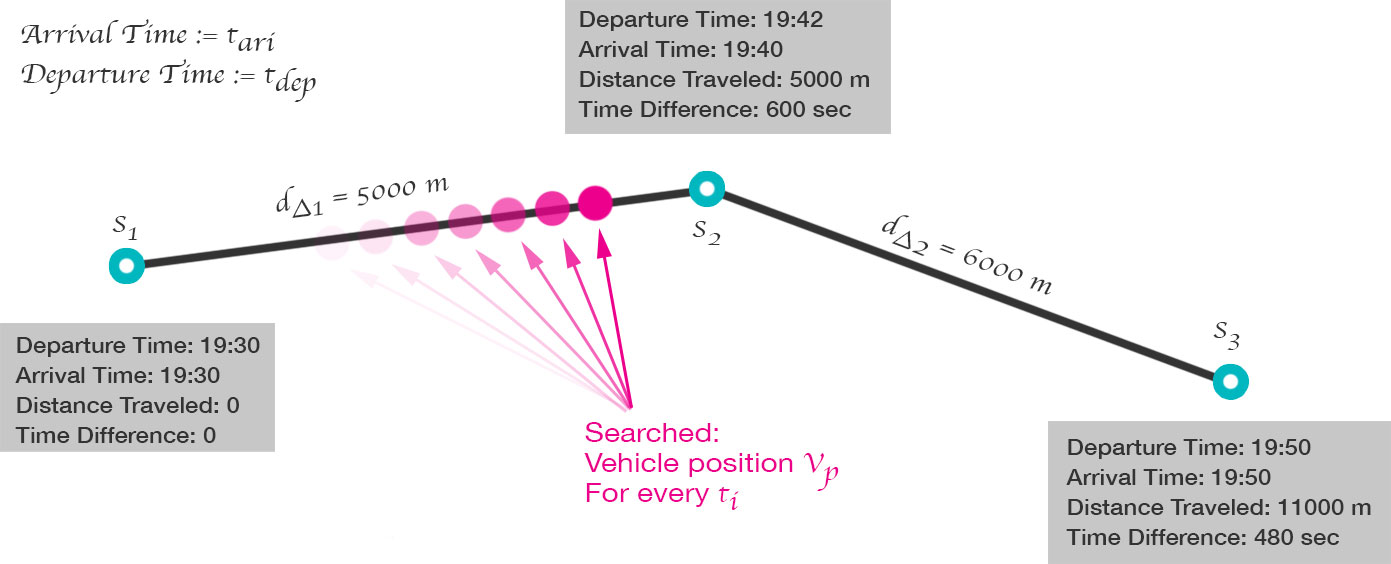
\includegraphics[width=0.9\textwidth]{interpolating_vehicle}
      \caption{Interpolation der Vehicle Position: $V_p$}
      \label{fig:interpolating_vehicle}
    \end{center}
  \end{figure}

  In den grauen Kästen der Grafik sind die Daten der einzelnen Stationen zu sehen. Diese kommen direkt aus der Datenbank oder werden vom Server vorberechnet und sind für die Berechnungen der Interpolation zwingend notwendig.
  \begin{itemize}[label={}]
    \item \textbf{Arrival Time:} Ankunftszeit $t_{ari}$ des Vehicles an der Station laut Fahrplan

    \item \textbf{Departure Time:} Abfahrtszeit $t_{dep}$ des Vehicles von der Station laut Fahrplan

    \item \textbf{Distance Traveled:} Bis zu dieser Station zurückzulegende Gesamtdistanz $d_S$

    \item \textbf{Difference Distance Traveled:} $d_\triangle$ ist die zurückzulegende Distanz zwischen 2 Stationen A und B\footnotemark

    \item \textbf{Time Difference:} Zeitdifferenz zwischen Ankunftszeit einer Station und der Abfahrtzeit der vorherigen Station $ TimeDifference = t_{ari_{S_n}} - t_{dep_{S_{n-1}}}$

  \end{itemize}

  \footnotetext{Als A und B seien immer zwei direkt aufeinander folgende Stationen $S_{n-1}, S_n$ bezeichnet.}

  Gesucht ist nun eine Vehicle Position $V_p$ zwischen den einzelnen Stationen für jede Zeiteinheit $t_i$. Dazu werden folgende Parameter benötigt:

  \begin{itemize}
    \item Aus der Datenbank wird die Polyline eines Trips benötigt. Auf dieser soll sich das Vehicle fortbewegen. Dieser Schritt wurde in Abschnitt \ref{sub:anzeigen_einer_polyline} bereits erläutert.

    \item Außerdem werden alle Stationen, die zu diesem Trip gehören, benötigt. Auch der Abruf dieser Informationen wurde im vorherigen Abschnitt bereits behandelt.

    \item Um die Vehicle Position ermitteln zu können, wird die Vehicle Geschwindigkeit $v$ benötigt. Um diese zu berechnen, wird die Formel $v = \frac{d_\triangle}{TimeDifference}$ für gleichförmige Bewegungen verwendet. Sowohl die Zeitdifferenz als auch $d_\triangle$ lässt sich aus dem GTFS Feed auf dem Server berechnen. Wie dies geschieht wird später in Kapitel "`\ref{ssub:station_matching} \nameref{ssub:station_matching}"' beschrieben.

    \item Mithilfe der berechneten Geschwindigkeit kann eine interpolierte Distanz $s_{neu}$ des Vehicles zu einem bestimmten Zeitpunkt berechnet werden, damit das Vehicle zwischen Station A und B bewegt werden kann. Dazu wird die Formel der gleichförmigen Bewegung $s_{neu} = v * t_i + s_0$ benötigt. $s_{neu}$ ist die interpolierte Distanz zwischen zwei Stationen A und B. $v$ ist die zuvor berechnete Vehicle Geschwindigkeit. $s_0$ ist die Anfangsdistanz und damit die \texttt{Distance Traveled} der vorherigen Station A. $t_i$ stellt eine Zeitdifferenz in Sekunden dar. Die Genauigkeit beträgt dabei Millisekunden, also beispielsweise $1.522 sec$. Diese wird errechnet, indem die \texttt{Departure Time} $t_{dep}$ der Station A von der momentanen Systemzeit der Webanwendung $t_{cur}$ subtrahiert wird. Dadurch lässt sich feststellen wann ein Trip aktiv oder inaktiv ist.

    Für $t_i < 0$ ergeben sich folgende Fälle: 
    \begin{itemize}[label={}]
      \item $t_{cur} < t_{ari_{S_1}} \Rightarrow$ Trip hat noch nicht begonnen und ist inaktiv

      \item $t_{ari_{S_{i}}} < t_{cur} < t_{dep_{S_i}} \Rightarrow$ Trip ist aktiv, aber Vehicle wartet an der Station auf weiterfahrt. 

      \item $t_{cur} > t_{dep_{S_n}} \Rightarrow$ Trip ist beendet
    \end{itemize}

    Für $t_i > 0 \Rightarrow$ der Trip ist aktiv und das Vehicle befindet sich zwischen zwei Stationen A und B.

  \end{itemize}
  
  Sind all diese Parameter vorhanden, lässt sich die Distanz des Vehicles zwischen den einzelnen Stationen zu jedem Zeitpunkt $t_{cur}$ interpolieren.
  Dafür kann die Bibliotheksfunktion \texttt{turf.along(polyline, $s_{neu}$)} verwendet werden, die eine Polyline und eine bestimmte Entfernung zum Startpunkt dieser Polyline nimmt und einen Punkt in dieser Distanz zurückgibt. Aus einer Distanz lässt sich also ein Punkt mit Längen und Breitengrad ausrechnen, der anschließend auf der Karte angezeigt werden kann. Erfolgt diese Berechnung eines neuen Punktes pro Sekunde 60 mal (was genau 60 FPS entspricht), so lässt sich durch das Verschieben dieses Punktes eine Animation des Vehicles erreichen. 

  \begin{figure}[htbp]
    \begin{center}
      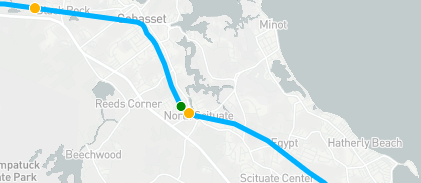
\includegraphics[width=0.4\textwidth]{prozess/animate_one_vehicle}
      \caption{Interpolation eines Vehicles entlang seiner Polyline}
      \label{fig:prozess/animate_one_vehicle}
    \end{center}
  \end{figure} 

  Das Ergebnis lässt sich in Abbildung \ref{fig:prozess/animate_one_vehicle} betrachten. Das Vehicle wird als grüner und die Stationen als orangene Kreise dargestellt.
  
% subsection animieren_eines_vehicles_durch_interpolation (end)
    \subsection{Zeichnen aller Polylines}
\label{sub:zeichnen_aller_polylines}
  Nachdem auf der Karte nun ein einzelner Trip angezeigt und animiert werden kann, sollte nun versucht werden, alle Polylines der Trips auf der Karte anzuzeigen. Abbildung \ref{fig:prozess/draw_all_shapes} zeigt, wie dies für das Boston MBTA-Feed aussieht.

  \begin{figure}[htbp]
    \begin{center}
      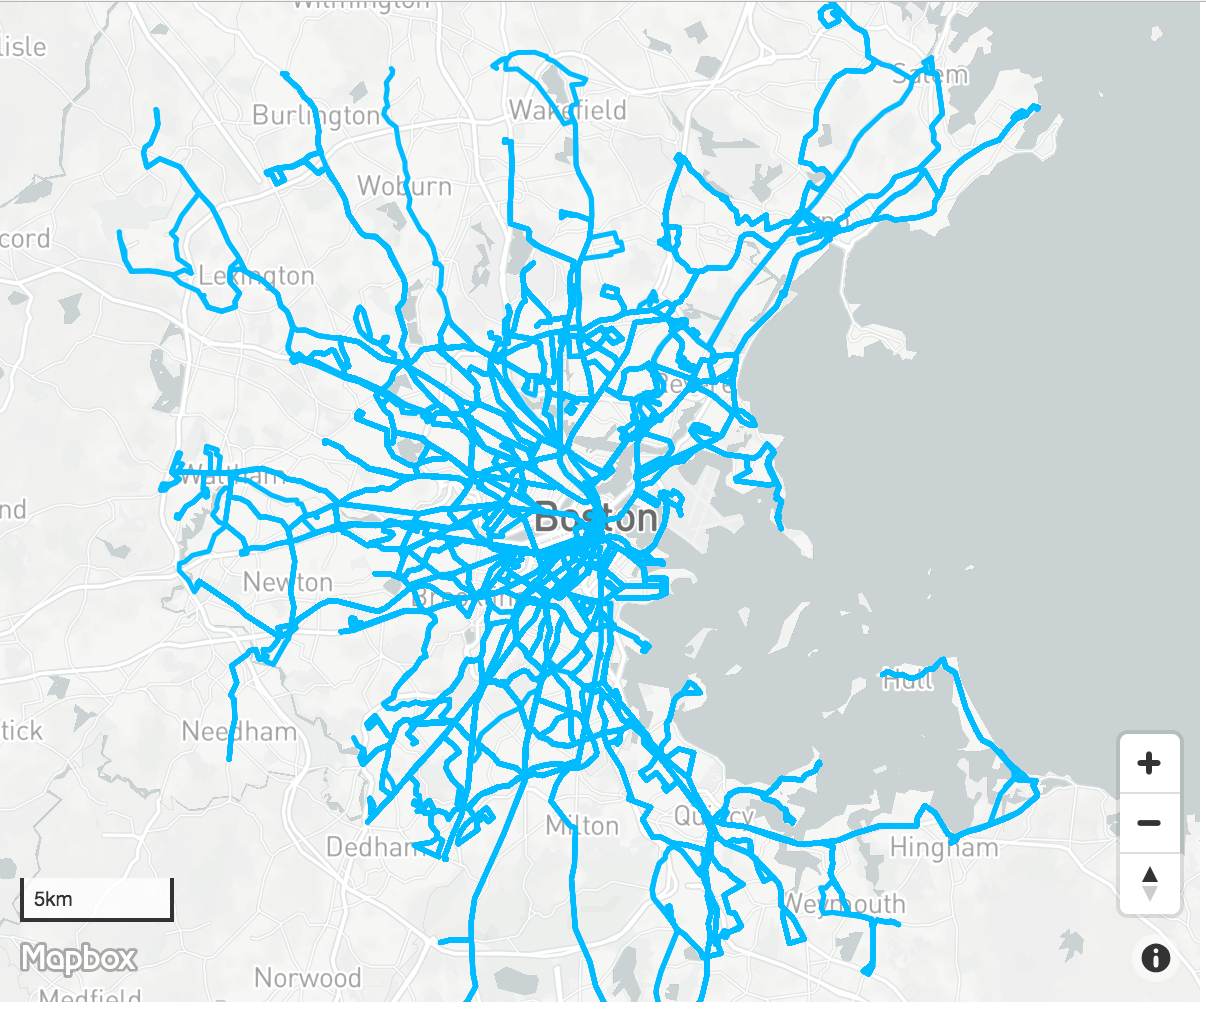
\includegraphics[width=0.5\textwidth]{prozess/draw_all_shapes}
      \caption{Darstellung aller Polylines auf der Karte}
      \label{fig:prozess/draw_all_shapes}
    \end{center}
  \end{figure}
  
  Zwar konnten alle Polylines auf der Karte angezeigt werden, allerdings bei sehr langer Rechen- und Ladezeit. Durch die Erhöhung der in der Datenbank abzufragenden Datenmenge, wurden neue Probleme offengelegt. Die ursprüngliche Datenrepräsentation der Polylines in der Datenbank war nicht optimal und die Daten ließen sich nicht performant genug abfragen. Im Folgenden sollen die Optimierungsmaßnahmen, welche an der Polyline und der Datenbank zur Steigerung der Performanz unternommen wurden, aufgezeigt werden.

  \subsubsection{Ramer–Douglas–Peucker}
  \label{ssub:ramer_douglas_peucker}
    Das Problem: Die im Stuttgart-VVS-Feed zur Verfügung gestellten Polylines sind überdefiniert und können aus tausenden Punkten bestehen. Für eine Visualisierung ist eine solche Genauigkeit nicht notwendig und aufgrund der großen Datenmenge problematisch. Durch die Verwendung des "`Ramer–Douglas–Peucker"' (RDP)-Algorithmus kann die Anzahl der Punkte einer Polyline drastisch reduziert werden. Der Vorteil besteht darin, dass dabei nicht der Linienverlauf verändert wird. Abbildung~\ref{fig:simplify} zeigt ein Beispiel einer solchen Vereinfachung mittels einer JavaScript Bibliothek\footnote{Simplify.js \url{http://mourner.github.io/simplify-js/}}.

    \begin{figure}[htbp]
      \centering
      \subfloat[Polyline vor RDP]{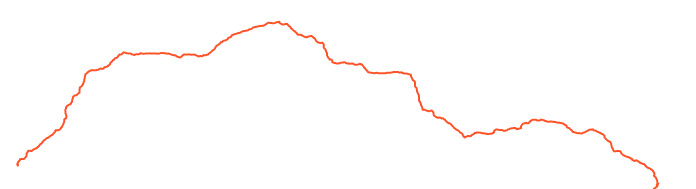
\includegraphics[width=0.48\textwidth]{simplify_before.jpg}\label{fig:simplify_before}}
      \hfill
      \subfloat[Polyline nach RDP]{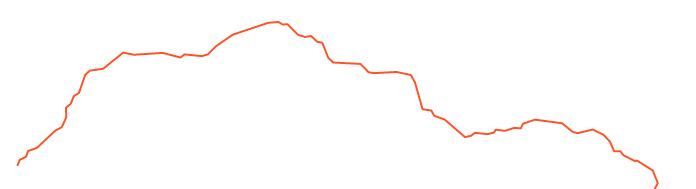
\includegraphics[width=0.48\textwidth]{simplify_after.jpg}\label{fig:simplify_after}}
      \caption{Vereinfachung einer Polyline mittels Simplify.js}
      \label{fig:simplify}
    \end{figure}

    Ausgangspunkt ist eine Polyline mit $\approx1000$ Punkten (\ref{fig:simplify}a). Nach der Vereinfachung (\ref{fig:simplify}b) ist die Anzahl auf 100 Punkte reduziert, ohne dabei visuell merklich einzubüßen. Dies ist eine erhebliche Reduzierung der Punkte um 90\%. Wie wirkt sich dieser Algorithmus positiv auf das Projekt aus? Die Vorteile sind weitreichend. Sehen wir uns die Shape-Tabelle in Abbildung \ref{fig:shape_simplify} an. \ref{fig:shape_simplify}a zeigt 394 Reihen vor der Optimierung und nur noch 140 (\ref{fig:shape_simplify}b) nach Anwendung des RDP Algorithmus.

    \begin{figure}[htbp]
      \centering
      \subfloat[Shape-Tabelle vor RDP]{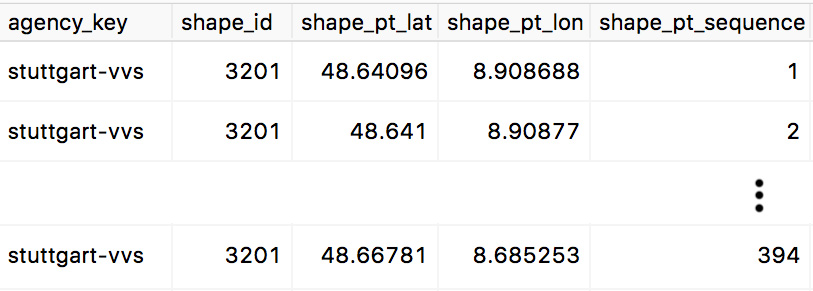
\includegraphics[width=0.48\textwidth]{shape_simplify_before.jpg}\label{fig:shape_simplify_before}}
      \hfill
      \subfloat[Shape-Tabelle nach RDP]{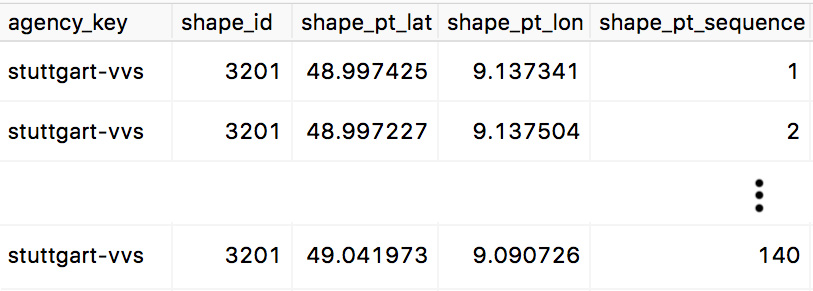
\includegraphics[width=0.48\textwidth]{shape_simplify_after.jpg}\label{fig:shape_simplify_after}}
      \caption{Reduzieren der Anzahl an Tabellen-Einträge via RDP}
      \label{fig:shape_simplify}
    \end{figure}

    In seinem Originalzustand hat das verwendete VVS-Feed 1,085,859 Mio. Zeilen. Nach der Anwendung sind diese auf 617,653 Tsd. verringert. Testet man folgende PostgreSQL Abfrage,
    \colorbox{materialGrey}{\texttt{\color{white}{{\color{materialBlue}SELECT} * {\color{materialBlue}FROM} gtfs\_shapes {\color{materialBlue}WHERE} shape\_id = {\color{materialRed}3201}}}}
    die alle Punkte einer Polyline ausgeben soll, so ergibt sich für ein optimiertes Feed eine Query-Zeit von $\approx145 ms$ und für das nicht optimierte Feed $\approx250 ms$. Schon durch diese einfache Methode sind bereits erste Performance-Steigerungen wahrnehmbar.\\

    Der RDP-Algorithmus wurde auf das GTFS-Feed angewendet, noch bevor die Daten der Polyline in die Datenbank importiert wurden. Dadurch muss die Polyline nicht während der Laufzeit vereinfacht werden, sodass diese Rechenzeit eingespart werden kann. In Kapitel \ref{ssub:gtfs_optimierungen} wird ein Tool namens \texttt{gtfstidy} vorgestellt, das GTFS-Feeds optimieren kann. Dabei ist auch das Vereinfachen von Polylines mittels RDP möglich.

  % subsubsection ramer_douglas_peucker (end)

  \subsubsection{Aggregieren der Shape-Tabelle}
  \label{ssub:aggregieren_der_shape_tabelle}
    In GTFS wird für jeden Punkt einer Polyline eine Reihe in der Datenbank belegt. Diese Abfolge ist durch eine sogenannte \texttt{Shape Point Sequence} festgelegt, was nichts anderes ist, als eine Zahl von $1$ bis $n$. Dies ist auch bereits in obiger Tabelle \ref{fig:shape_simplify} zu sehen gewesen. Sehr viel effektiver wäre es allerdings, diese Punkte nicht Reihenweise, sondern alle zusammengehörenden Punkte in nur einem einzigen Feld zu speichern. Dies ist in PostgreSQL durch eine Aggregierung möglich. Daraus ergibt sich folgende Shape-Tabelle:\\

    \begin{figure}[htbp]
      \begin{center}
        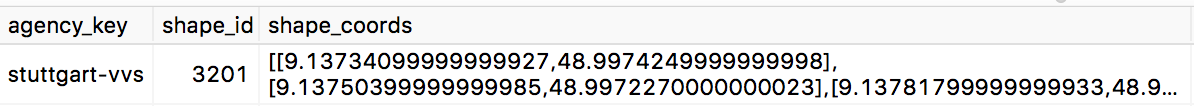
\includegraphics[width=\textwidth]{aggregated.png}
        \caption{Aggregierte Koordinaten der Shape-Tabelle}
        \label{fig:aggregated}
      \end{center}
    \end{figure}

    Wie zu sehen ist, benötigt nun eine Polyline in der Shape-Tabelle nicht mehr 140 Reihen, sondern nur noch eine einzige. Für diese Arbeit ist dies auf alle Polylines angewendet worden und in einer neuen Tabelle namens \texttt{denormalized\_shapes} abgespeichert. Dadurch ist die Berechnung der Aggregierung nur einmal nötig. Der SQL-Befehl dafür ist dem Anhang unter \ref{lst:sql_aggregate_shape} zu entnehmen.
    Wir wenden die selbe SQL-Abfrage, die bereits oben Verwendung fand, auf die neue \texttt{denormalized\_shapes} Tabelle an. Die Query-Zeit ist auf $\approx1ms$ gesunken. Anstatt hunderte Reihen, muss nur eine einzige Reihe ausgelesen werden, was sehr effizient ist. Durch das Denormalisieren\footnotemark der Shape-Tabelle ist auch die Anzahl der Reihen in der Datenbank auf ein Minimum gesunken. Von den früheren 617,653 Tsd. Reihen sind durch die Aggregation nur noch 4,524 Tsd. übrig.

    \footnotetext{Denormalisieren beschreibt den Prozess der Relationsauflösung von Datenbanktabellen.}
  
  % subsubsection aggregieren_der_shape_tabelle (end)

  \subsubsection{Polyline Encoding}
  \label{ssub:polyline_encoding}
    Die letzte Maßnahme zur Optimierung der Polyline stellt das sogenannte Polyline-Encoding dar. Wie dieses Verfahren genau funktioniert, geht an dieser Stelle zu weit. Hier soll nur erklärt werden, was unter Polyline-Encoding verstanden wird und warum es hier angewandt wird.\\

    Das Polyline-Encoding kann in JavaScript beispielsweise durch das Google-Polyline\footnote{\url{https://www.npmjs.com/package/google-polyline}} Paket eingesetzt werden. Das Encoding wandelt eine Polyline, bestehend aus Punkten, in einen String um. Zum Beispiel die Punkte: (38.5, -120.2), (40.7, -120.95), (43.252, -126.453) werden als
    \colorbox{materialGrey}{\texttt{\color{white}{\_p\textasciitilde iF\textasciitilde ps|U\_ulLnnqC\_mqNvxq`@}}}
    codiert. Dies geschieht in meiner Anwendung immer bevor Daten vom Server in Richtung Client geschickt werden: Encode $\rightarrow$ Send $\rightarrow$ Decode. Da eine codierte Polyline weniger Zeichen benötigt, kann damit Datenvolumen bei der Kommunikation zwischen Server und Client gespart werden.

  % subsubsection polyline_encoding (end)
% subsection zeichnen_aller_polylines (end)
    \subsection{Anzeigen aller Stationen}
\label{sub:anzeigen_aller_stationen}

  Nachdem zuvor alle Trips mit ihren Polylines in der Karte angezeigt wurden, folgt nun das Anzeigen aller Stationen, die zu einem Trip gehören. Änlich wie beim Abfragen und Anzeigen aller Polylines, sollte dieser Schritt mögliche Engpässe oder unvorhergesehene Probleme aufdecken (Abbildung \ref{fig:prozess/draw_all_stations}).

  \begin{figure}[htbp]
     \begin{center}
       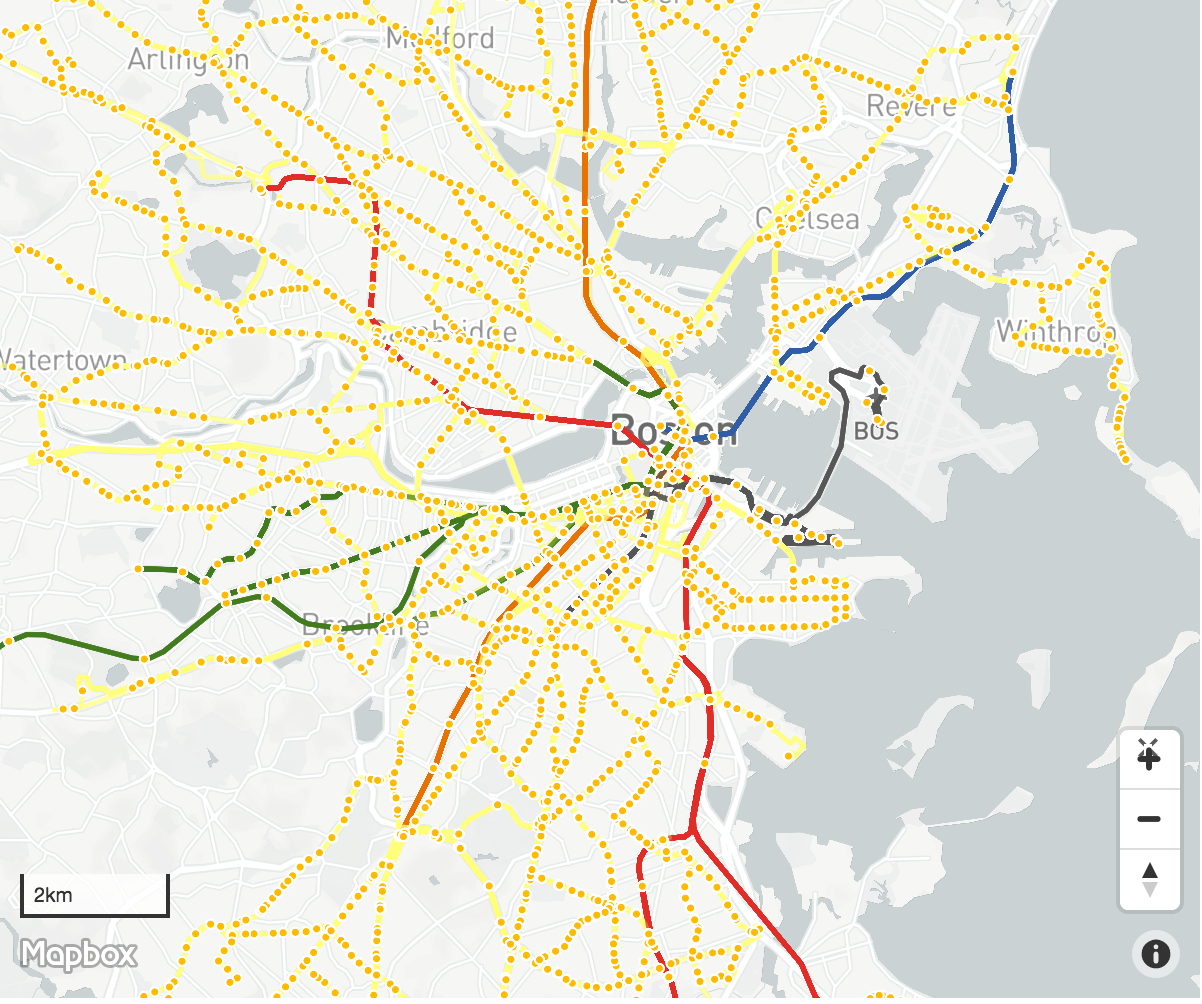
\includegraphics[width=0.6\textwidth]{prozess/draw_all_stations}
       \caption{Aktive Trips mit ihren dazugehörenden Stationen}
       \label{fig:prozess/draw_all_stations}
     \end{center}
   \end{figure}
   
  Vor allem die Abfrage von aktiven Trips aus der Datenbank, stellte ein großes Problem dar. Die Datenbank konnte die Anfragen des Clients nicht effizient genug verarbeiten. An dieser Stelle stand fest, dass für die weitere Arbeit umfassende Optimierungen der Datenbank erfolgen müssen, um eine responsive Webanwendung zu ermöglichen. 

  \subsubsection{GTFS Optimierungen}
  \label{ssub:gtfs_optimierungen}
    Der erste Schritt um die Performance zu verbessern, ist die Optimierung von GTFS Feeds. Damit lässt sich die Datenmenge bereits vor dem Importieren in die Datenbank, erheblich verringern. Ein Tool um ein GTFS Feed umfassend zu optimieren ist \texttt{gtfstidy} \url{https://github.com/patrickbr/gtfstidy}. Es bietet dabei allerdings nicht nur die Möglichkeit für die Vereinfachung von Polylines sondern kommt mit einer ganzen Reihe an Optimierungsmöglichkeiten. 

    Der Kommandozeilenbefehl \colorbox{materialGrey}{\texttt{\color{white}{\$ gtfstidy -sSiRDeO input.zip output}}} optimiert das Stuttgart-VVS Feed wie folgt:
    
    \begin{itemize}[label={}]
      \item \textbf{-s} Reduziert die Punktanzahl einer Polyline
        
      \item \textbf{-S} Entfernt redundante Polylines.

      \item \textbf{-i} Umwandlung von Zeichen ID's (String) in Zahlen ID's (Integer).\footnote{Aus der String ID \texttt{'1.T0.10-1-j17-1.16.H'} wird \texttt{78}}

      \item \textbf{-O} Entfernt Feed Einträge die nicht referenziert werden.

      \item \textbf{-R} Entfernt doppelt vorhandene Routen.

      \item \textbf{-e} Setzt fehlerhafte oder optionale Felder auf einen Standard Wert.

      \item \textbf{-D} Entfernt fehlerhafte Einträge aus dem Feed.
    \end{itemize}

    Durch Verwendung von gtfstidy konnte das Feed optimiert werden und die Datengröße der einzelnen Dateien um folgendes Maß verringert werden.

    \begin{longtable}{|>{\raggedright \arraybackslash}p{5.0cm}|>{\raggedright \arraybackslash}p{5.0cm}|>{\raggedright \arraybackslash}p{5.0cm}|}
      \hline
      Dateiname & Größe davor& Größe danach\\
      \hline
      trips.txt & 6 MB & 2.8 MB\\
      stop\_times.txt & 103 MB & 53 MB\\
      stops.txt & 651 KB & 355 KB\\
      shapes.txt & 77.3 MB & 22.4 MB\\
      routes.txt & 54 KB & 38 KB\\
      calendar\_dates.txt & 557 KB & 463 KB\\
      \hline
      \caption{Tabellengröße bevor und nach anwenden von gtfstidy}
      \label{tbl:gtfs_tidy_results}
    \end{longtable}

    Insgesamt konnte so die Größe des Feeds von 79 MB auf 118 MB um knapp 50\% verringert werden. Vor allem die Umwandlung von langen String ID's in kürzere Integer ID's trägt maßgeblich zur Verringerung der Dateigröße bei.

  % subsubsection gtfs_optimierungen (end)

  \subsubsection{Denormalisierung der Datenbank}
  \label{ssub:denormalisierung_der_datenbank}
    Die Denormalisierung ist eine Strategie, die auf eine zuvor normalisierte Datenbank angewendet wird, um die Leistung zu erhöhen. Die Denormalisierung ist der Prozess, bei dem versucht wird, die Leseperformance einer Datenbank zu verbessern, auf Kosten der Schreibleistung, durch Hinzufügen redundanter Kopien von Daten oder durch deren Gruppierung.\parencite{sanders}
    Der große Nachteil von Denormalisierung, nämlich die Redundanz von Daten, spielt für dieses Projekt keine Rolle, da die Daten ausschließlich ausgelesen und nicht geschrieben werden. Was bleibt sind die Vorteile.\\

    Für dieses Projekt bedeutet diese Methode, eine neue Tabelle zu generieren, die den Zugriff auf die benötigten Daten einfach macht. Im Grunde handelt es sich um eine Vorberechnung. Anstatt die Tabellen bei jeder Anfrage an den Server aufwendig über viele \texttt{SQL-JOINS} zu verknüpfen, wird diese Verknüpfungen einmalig vorberechnet und in eine Tabelle gespeichert. Eine Denormalisierung  einer Tabelle ist bereits im vorherigen Abschnitt "`\nameref{ssub:aggregieren_der_shape_tabelle}"' gezeigt und führte dazu, dass die Polyline über die Abfrage einer einzigen Tabellenreihe erhalten werden kann was die Performance signifikant erhöhte. Zur besseren Verständnis soll folgende Grafik helfen:

    \begin{figure}[htbp]
      \begin{center}
        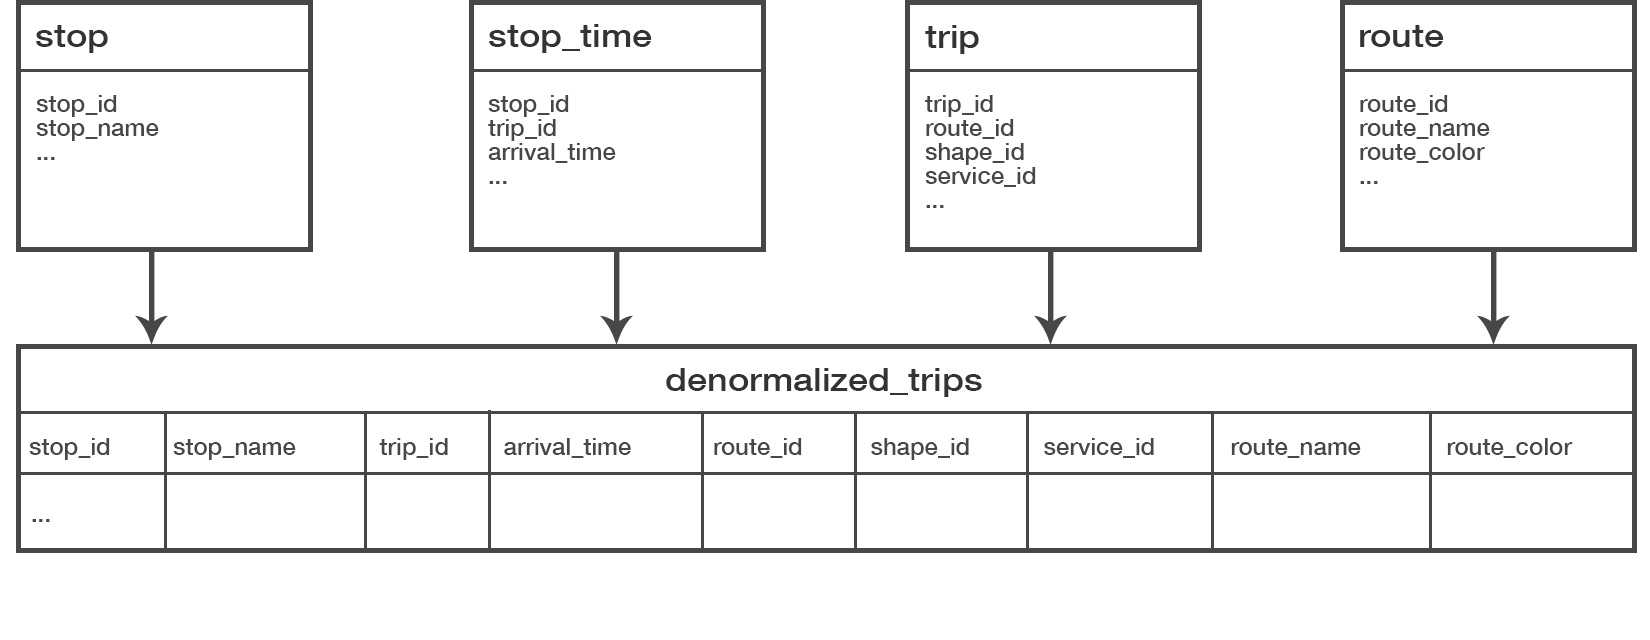
\includegraphics[width=\textwidth]{denormalizing.jpg}
        \caption{Beispiel einer Denormalisierung von Tabellen}
        \label{fig:denormalizing}
      \end{center}
    \end{figure}

    Wie in Abbildung \ref{fig:denormalizing} zu sehen ist, wird aus einer vertikalen Anordnung der einzelnen Datenfelder, eine horizontale Anordnung in einer einzigen \texttt{denormalized\_trips} Tabelle. Eine Reihe in dieser neuen Tabelle steht für genau einen Eintrag eines Trips. Anstatt also bei jeder Anfrage an den Server die verschiedenen Daten mittels \texttt{JOIN} verknüpfen zu müssen, können diese jetzt per Zugriff auf eine einzige Reihe in nur einer Tabelle erfragt werden.

    Dieses Prinzip, der Gruppierung von Daten in einer neuen Tabelle soll nun auch auf die anderen benötigten Tabellen angewendet werden. Die Denormalisierung erfolgt in 3 Schritten:

    \begin{enumerate}
      \item Erstellen der neuen Tabelle \texttt{denormalized\_trips}
      \item Importieren der verschiedenen Daten in diese neue Tabelle
      \item Mögliche Abfragen sind nun über diese neue Tabelle möglich.
    \end{enumerate}

    Das SQL-Statement ist abermals aufgrund seiner Länge Anhang \ref{lst:denormalized_shapes} zu entnehmen. Dies resultiert in einer Tabelle die wie folgt aussieht:

    \begin{figure}[htbp]
      \begin{center}
        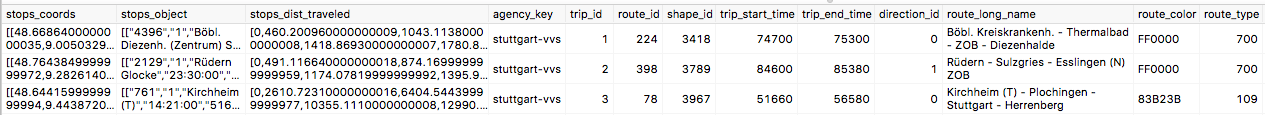
\includegraphics[width=\textwidth]{denormalized_tables.png}
        \caption{Auszug aus der \texttt{denormalized\_trips} Tabelle}
        \label{fig:denormalized_table}
      \end{center}
    \end{figure}  

    \subsubsection*{Ergebnisse der Denormalisierung}
    \label{ssub:ergebnisse_der_denormalisierung}
      Für die Visualisierung ist eine Abfrage der aktiven Trips am wichtigsten.
      Folgende Tabellen werden für die Abfrage benötigt.

      \begin{figure}[htbp]
        \begin{center}
          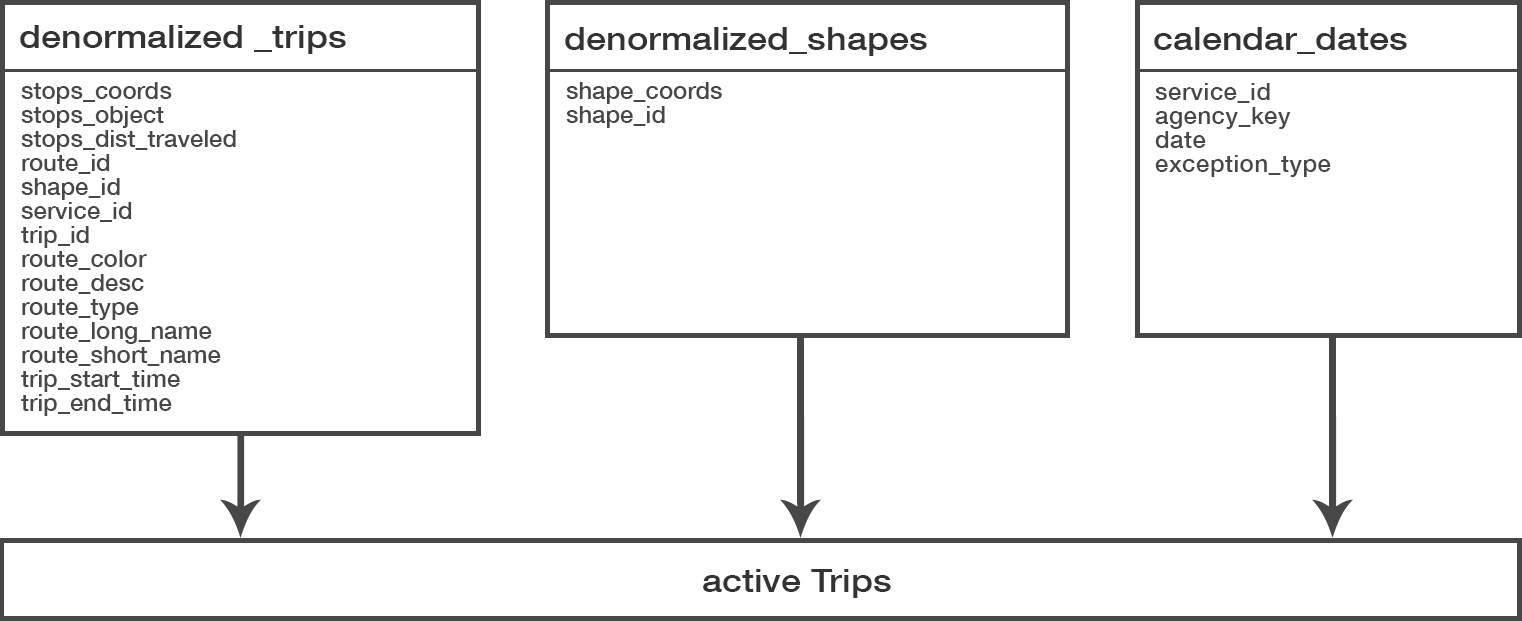
\includegraphics[width=\textwidth]{denormalizing_results.jpg}
          \caption{Benötigte Tabellen zur Abfrage von Trips}
          \label{fig:denormalizing_results}
        \end{center}
      \end{figure}

      Wie zu sehen ist, wird auf die Denormalisierte \texttt{Shape} und \texttt{Trips} Tabelle zugegriffen.

      Nachfolgend die Ergebnisse für die Abfrage von Trips in einem wachsenden Zeitrahmen. Die verwendete SQL-Abfrage befindet sich im \nameref{sec:anhang} unter Listing \ref{lst:query_trips}.

      \begin{longtable}{|>{\raggedright \arraybackslash}p{5.0cm}|>{\raggedright \arraybackslash}p{5.0cm}|>{\raggedright \arraybackslash}p{4.0cm}|}
      \caption{Evaluierung der Denormalisierung}\label{tbl:evaluierung_der_denormalisierung}\\
        \hline
          Zeitraum & Trip Anzahl & Query Zeit\\
        \hline
          9:00 bis 9:15 & 88 & 98 ms\\
          9:00 bis 10:00 & 1125 & 154 ms\\
          9:00 bis 12:00 & 3360 & 285 ms\\
          9:00 bis 15:00 & 7070 & 497 ms\\
          9:00 bis 21:00 & 14718 & 900 ms\\
        \hline
      \end{longtable}

      Die Ergebnisse Zeigen, dass die Abfragezeit der Datenbank für die aktiven Trips erheblich gesunken ist. Anfangs ist solch eine Anfrage aufgrund der endlosen Laufzeit erst gar nicht möglich gewesen.

      \begin{figure}[htbp]
        \begin{center}
          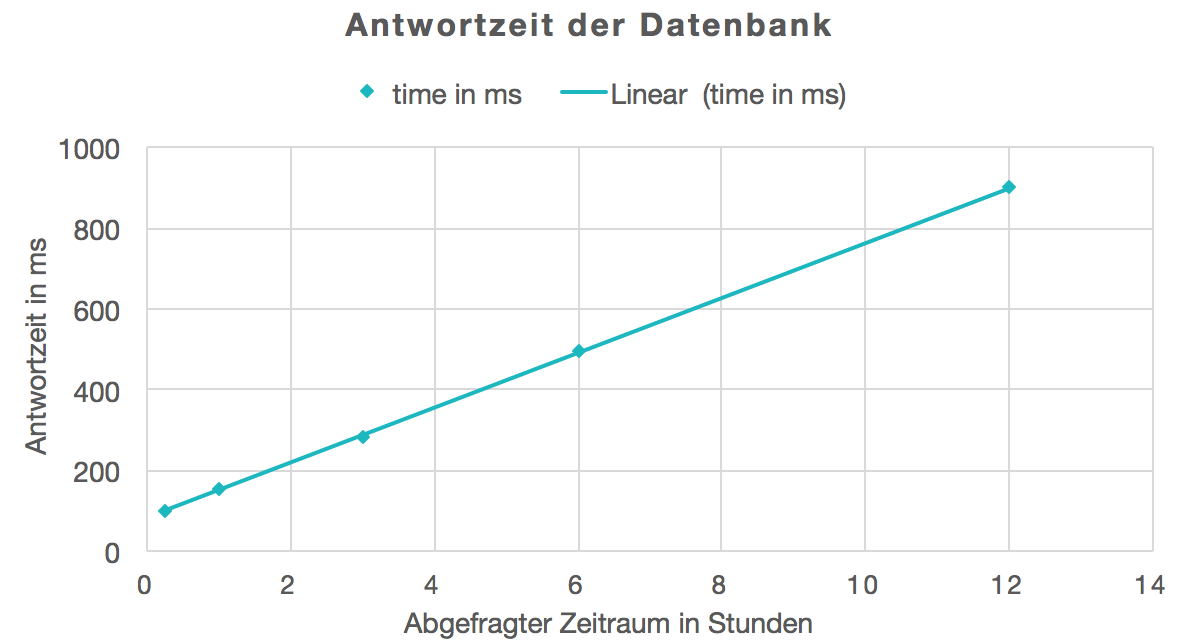
\includegraphics[width=0.7\textwidth]{query_time_chart}
          \caption{Plot der Abfragezeiten}
          \label{fig:query_time_chart}
        \end{center}
      \end{figure}
      
      Abbildung \ref{fig:query_time_chart} zeigt einen Plot der Query Zeit aus Tabelle \ref{tbl:evaluierung_der_denormalisierung} als linearen Graphen. Daraus folgt, dass die Antwortzeit der Datenbank linear mit dem abgefragten Zeitraum wächst. Für die Visualisierung sind vor allem zwei Abfragen wichtig: Erstens das Abfragen eines größeren Zeitraums von 1-2 Stunden. Dies geschieht beim ersten Aufrufen der Webanwendung wenn die Karte noch keine Trips besitzt und damit leer ist. Zweitens die Abfrage von nur kleinen Zeiträumen von nur einer Minute, um neue Trips abzufragen. Für diese zwei Abfragen bewegt sich die Antwortzeit des Servers zwischen $\approx 80 -  160\; ms$. Damit wurde das in Kapitel \ref{sub:zielsetzung} gesetzte ziel von 0 bis $200ms$ bereits erreicht.
      
    % subsubsection ssub:ergebnisse_der_denormalisierung (end)
  % subsubsection denormalisierung_der_datenbank (end)
% subsection anzeigen_aller_stationen (end)
    \subsection{Animieren der aktiven Trips}
\label{sub:animieren_der_aktiven_trips}
  Nachdem die Daten für alle aktiven Trips im Client ankommen, kann für jeden Trip ein Vehicle erstellt werden. In einem Animation-Loop wird für jedes Vehicle pro Frame, eine neue Position berechnet und die Karte wird mit der neuen Position aktualisiert. Der Algorithmus dafür ist in Pseudo-Code in Listing \ref{alg:animate_algorithmus} beschrieben.

  \begin{algorithm}[H]
    \caption{Animate Vehicle}\label{alg:animate_algorithmus}
    \begin{algorithmic}[1]
      \Procedure{animateVehicle}{}
        \State ServerQueryTimer $\gets$ 30 Seconds
        \State Vehicles $\gets$ Vehicles Inside Bounding Box
        \State Trips $\gets$ Requested Trips
        \Function{animate}{timestamp}
          \ForAll{Vehicles as Vehicle} \State{
            \If{Vehicle started its Trip} 
              \State \Call{calculateVehiclePosition}{Vehicle}
            \EndIf
            \If{Vehicle not started its Trip}
              \State \Call{checkVehicleActivity}{Vehicle, Trips}
            \EndIf
            \State \Call{checkIfVehicleHasFinished}{Vehicle}
            \State \Call{updateMapWithNewPositions}{Vehicles}
          }\EndFor

          \If{ServerQueryTimer Expired} 
            \State Query Server for New Trips
            \State ServerQueryTimer $\gets$ 30 Seconds
          \EndIf

          \State \Call {animate}{timestamp}
        \EndFunction
        
      \EndProcedure
    \end{algorithmic}
  \end{algorithm}

  Innerhalb dieses Animation-Loops passieren mehrere Dinge. Zuerst wird geprüft ob sich ein Vehicle überhaupt im Sichtbereich des Anwenders befindet. Trifft das zu, wird für eben diese Vehicle die Distanzen berechnet und die Position des Vehicles entlang der Polyline interpoliert. Falls das Vehicle seinen Trip noch nicht begonnen hat, wird überprüft ob das immer noch der Fall ist. Anschließend werden alle Vehicle geprüft, ob sie ihren Trip erledigt haben. Danach wird die Karte mit den neuen Positionen der Vehicle aktualisiert. Während all dies geschieht, läuft ein Timer mit, der nach dem Ablaufen von 30 Sekunden den Server nach neuen Trips abfrägt.

  Das Ergebnis ist die Animation aller Vehicle der momentan aktiven Trips (Abbildung \ref{fig:prozess/animate_all_vehicles}).

  \begin{figure}[htbp]
    \begin{center}
      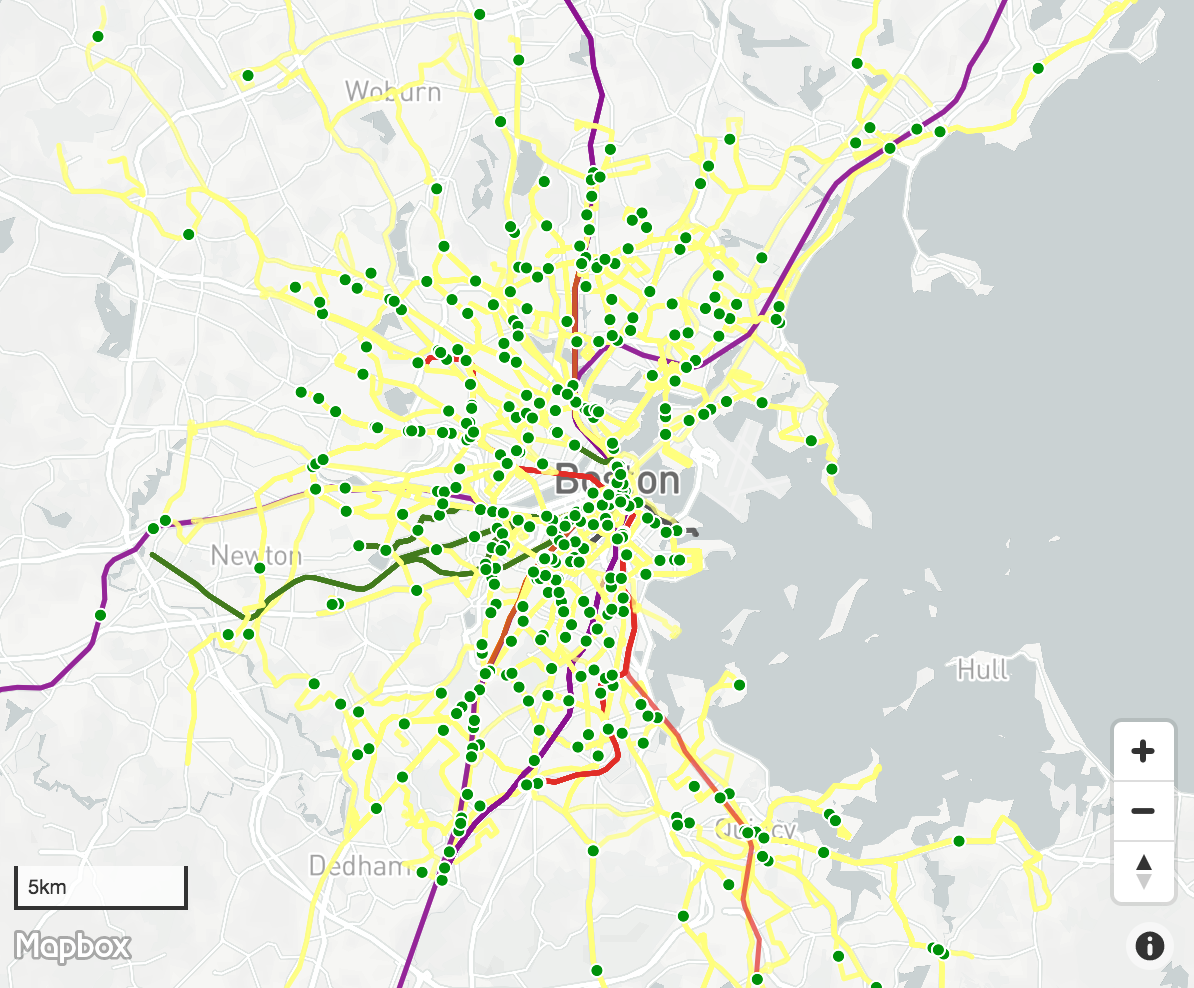
\includegraphics[width=0.7\textwidth]{prozess/animate_all_vehicles}
      \caption{Animieren aller Vehicles auf der Karte}
      \label{fig:prozess/animate_all_vehicles}
    \end{center}
  \end{figure}
  
  
  
% subsection animieren_der_aktiven_trips (end)

  % section develop (end)
\end{newpage}

  \begin{newpage}
  \section{Deliver}
  \label{sec:deliver}

    In diesem Kapitel sollen das Endprodukt und seine Funktionsweise im Gesamtzusammenhang vorgestellt werden. Der erste Abschnitt widmet sich dem generellen Funktionsprinzip und der Kommunikation zwischen Server und Client, bevor im zweiten Abschnitt die einzelnen Funktionen der fertigen Webanwendung beschrieben werden. Im letzten Abschnitt wird schließlich überprüft, inwiefern die Zielsetzungen bezüglich der Performance erreicht werden konnten. 
    
    \subsection{Funktionsprinzip}
\label{sub:funktionsprinzip}
    Für einen Datenaustausch zwischen Server und Client, sind in der fertigen Webanwendung folgende API\footnotemark-Endpunkte vorhanden. 

    \footnotetext{Application Programming Interface}

    \begin{itemize}
      \item \textbf{/daily} stellt die Daten für das Zeitstrahldiagramm bereit und wird beim Start der Anwendung einmalig angefragt. Die Antwort enthält XY-Wertpaare. X stellt dabei die Zeit in Sekunden und Y die zu diesem Zeitwert aktiv werdenden Trips dar.

  \begin{lstlisting}[captionpos=t, caption=Antwort des Servers zur Anfrage \texttt{/daily}, label=lst:daily_response]
  [
    {"x":86340,"y":"6"},
    {"x":86400,"y":"10"}, 
    ...
  ]
  \end{lstlisting}

      \item \textbf{/trips/:from,:to} ermöglicht das Abfragen von Trips, die in einer Zeitspanne \texttt{from - to} aktiv sind. Beim initialen Aufruf der Webanwendung wird dieser Endpunkt als Erstes angefragt, um die aktiven Trips innerhalb einer Stunde zu erhalten. Der gewählte Zeitraum ist in Sekunden anzugeben. 

      Die Antwort des Servers auf einen Endpunkt vom Typ \texttt{/trips/} ist ein Objekt mit der Trip\_Id, dessen Inhalt der \texttt{GeoJSON} Spezifikation nach RFC 7946 folgt:

  \begin{lstlisting}[captionpos=t, caption=Trip Objekt, label=lst:trip_object]
  {
    2498: {  
      "type": "FeatureCollection",
      "features": [
        {
          "type": "Feature",
          "properties": {
            "name": "shape",
            ...
          },
          "geometry": {
            "type": "LineString",
            "coordinates": [[9.4437,48.64482], ...]
          }
        },
        {
          "type": "Feature",
          "properties": {
            "name": "station"
          },
          "geometry": {
            "type": "Point",
            "coordinates": [9.443688, 48.6448]
          }
        },
        ...
      ]
    }
  }
  \end{lstlisting}
    
      Da die Antwort in Listing \ref{lst:trip_object} mittels "`..."' gekürzt ist, sind detailliertere Antworten im \nameref{sec:anhang} unter Listing \ref{lst:geojson_featurecollection}, \ref{lst:shape_feature} und \ref{lst:station_feature} zu finden.

      \item \textbf{/trips/:id} antwortet mit den zur ID gehörenden Trip-Informationen. Dieser Endpunkt ermöglicht es, Informationen für nur einen einzigen Trip zu bekommen. Dies ist vor allem dann hilfreich, wenn der Nutzer ein Vehilce anklickt und Informationen über diesen Trip angezeigt bekommen möchte. Beispiel: \texttt{/trips/51295}

      \item \textbf{/trips/new/:from,:to,:tripIds} stellt die Abfrage für neue Trips zur Verfügung und exkludiert dabei diejenigen Trips, die in \texttt{:tripIds} genannt sind. Damit wird verhindert, dass bereits auf der Karte vorhandene Trips nicht doppelt auftauchen können. Diese Datenbankabfrage wird in einem 30-Sekunden-Intervall vom Client an den Server gesendet, um die neusten Trips zu erhalten. Damit wird die Karte aktuell gehalten. Beispiel: Es ist 10:00 Uhr, hole die in der nächsten Minute aktiv werdenden Trips (Zeitraum 10:00 bis 10:01 Uhr) und schließe die Trips mit der ID \texttt{51295,9212,52} vom Ergebnis aus \texttt{/trips/new/36000,36060,51295,9212,52}.

      \item \textbf{/trips/new/:from,:to} stellt die gleiche Funktionalität wie der vorherige Endpunkt zur Verfügung, mit der Ausnahme, dass keine Trip-ID's übermittelt werden müssen. Dieser Endpunkt ist beispielsweise dafür da, falls die Karte leer ist und noch keine aktiven Trips enthält.

    \end{itemize}

  % subsubsection api_endpunkte (end)

  Das generelle Prinzip der Webanwendung beruht auf einer Client / Server Architektur. Der Nodejs-Server stellt verschiedene Endpunkte mittels Express als ansprechbare Routen dem Client zur Verfügung. 

  \begin{figure}[htbp]
    \begin{center}
      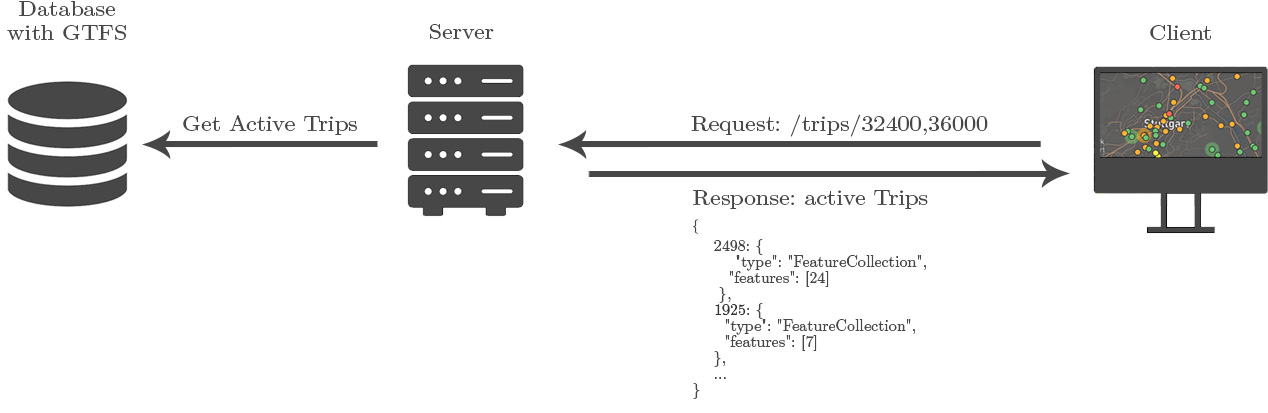
\includegraphics[width=\textwidth]{server_client.jpg}
      \caption{Server / Client Relation}
      \label{fig:server_client}
    \end{center}
  \end{figure}

  Trifft eine valide Anfrage auf den \texttt{/trips/:from,:to} Endpunkt, so wird ein Ablauf nach Abbildung \ref{fig:server_client} angestoßen.
  Die eintreffenden Anfragen werden vom Server entgegengenommen, validiert, verarbeitet und anschließend die entsprechende Antwort zurückgesendet. Die Validierung prüft die vom Client übergebenen Parameter auf ihre Plausibilität. Schlägt diese Prüfung fehl, wird ein Fehler vom Server zurückgegeben und der Server wartet auf eine neue Anfrage. Die wichtigste Routine des Servers stellt die Abfrage von Trips aus der Datenbank dar. Die Datenbank sucht diejenigen Trips heraus, welche in dem benötigten Zeitraum \texttt{from, to} aktiv sind. Dabei wird das Datum und der Wochentag zum Zeitpunkt der Anfrage verwendet. Um die Rechenarbeit im Client zu minimieren, werden alle Daten bei denen dies möglich ist, auf dem Server vorberechnet. Die aus der Datenbank abgefragten Daten durchlaufen folgenden Transformationsprozess:

  \begin{itemize}
    \item \textbf{Daten Mapping:} Die Trips aus der Datenbank werden in das \texttt{GeoJSON}-Format umgewandelt, damit diese im weiteren Programmverlauf einfacher zu verarbeiten sind. Dabei werden die im Kapitel "`\ref{sub:begriffe} \nameref{sub:begriffe}"' festgelegten Regeln beachtet.

    \item \textbf{Zurückgelegte Distanz:} Damit eine Animation der Vehicle stattfinden kann, ist die Berechnung der Distanzen zwischen den einzelnen Stationen nötig. 

    Falls das Feld dist\_traveled\footnotemark in der Datenbank vorhanden ist, kann die zurückgelegte Distanz sehr einfach daraus berechnet werden. Ist dies nicht der Fall, so wird das in Abschnitt \ref{ssub:station_matching} beschriebene Station-Matching durchgeführt, um die Distanzen berechnen zu können.
    \footnotetext{Die zurückgelegte Distanz bis zu einer Station $S$}

    \item \textbf{Feststellen der Richtung:} Für eine Polyline ist es unerheblich, ob die Koordinaten in der Reihenfolge $\{ p_1, p_2, \dotsc, p_n \}$ oder $\{ p_n, \dotsc, p_2, p_1 \}$ angeordnet sind. Damit das Vehicle aber in die richtige Richtung von $A$ nach $B$ fährt, ist es wichtig, dass die Koordinaten der Polyline in aufsteigender Reihenfolge festgelegt werden. Falls dies nicht der Fall ist, werden die Koordinaten in ihrer Reihenfolge umgekehrt.

    \item \textbf{Zeit zwischen Stationen:} In diesem Schritt wird die Fahrzeit (in sec) zwischen den einzelnen Stationen der Trips vorberechnet.

    \item \textbf{Codieren der Polyline:} Hier werden die Koordinaten in einen Polyline-String codiert.

    \item \textbf{Versenden:} Zuletzt wird die Anfrage des Clients vom Server mit einem Response-Paket beantwortet und der Prozess ist damit abgeschlossen bis eine neue Anfrage den Server erreicht.
  \end{itemize}
    
% subsection funktionsprinzip (end)
    \subsection{Funktionen der Webanwendung}
\label{sub:funktionen_der_webanwendung}
  In diesem Abschnitt sollen die verschiedenen UI-Komponenten vorgestellt werden.

  \subsubsection*{Die Karte}
  \label{ssub:die_karte}
    Die Karte (\ref{fig:map}) ist standardmäßig auf den Längengrad 9.244 und Breitengrad 48.757 ausgerichtet. Damit findet sich der Anwender beim Aufrufen der Applikation gleich an der richtigen Stelle wieder. Die Karte verwendet eine abgeänderte Version des Kartenstils \texttt{Mapbox-Dark}. Dabei wurden Parks, Grünflächen und Wasser subtil eingefärbt und die Routen des GTFS-Feeds mit einem leichten Orange hervorgehoben.

    \begin{figure}[htbp]
      \begin{center}
        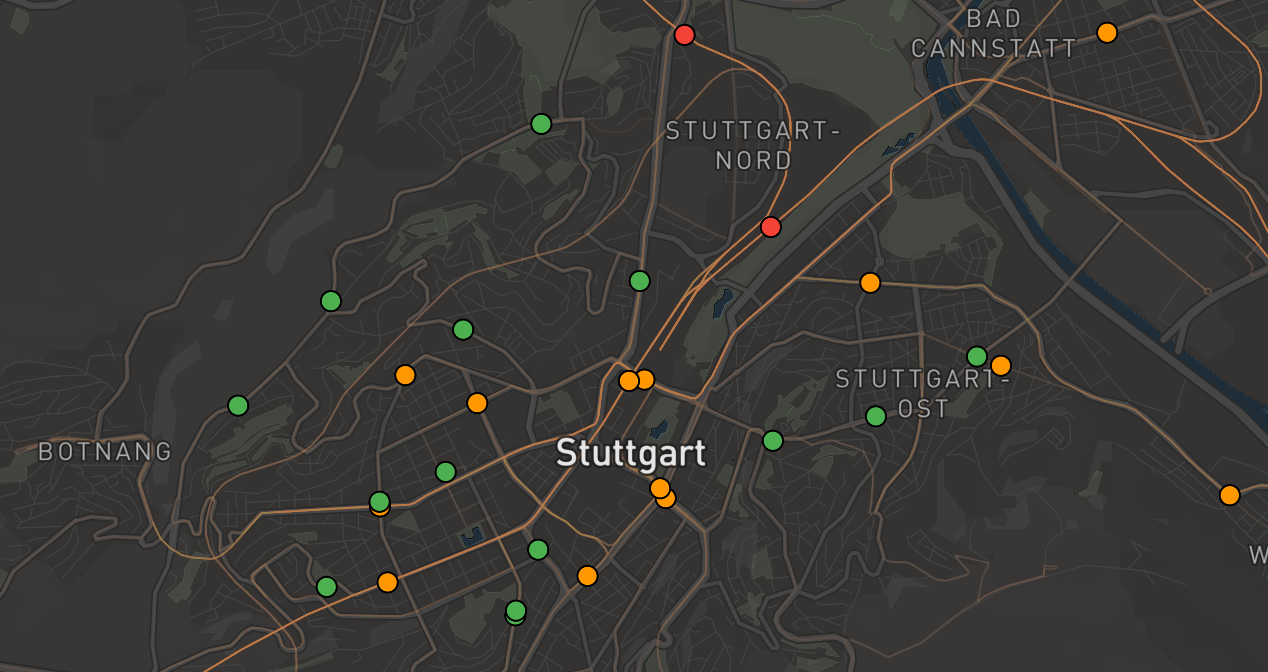
\includegraphics[width=0.6\textwidth]{map}
        \caption{Die Karte mit angepasstem Style: Mapbox-Dark}
        \label{fig:map}
      \end{center}
    \end{figure}
    
  % subsubsection die_karte (end)

  \subsubsection*{Vehicle}
  \label{ssub:vehicle_auf_karte}
    Die Vehicle sind auf der Karte als Kreis dargestellt. Die verwendete Farbe orientiert sich dabei an den offiziellen Farben des jeweiligen Verkehrsunternehmens. Zum Beispiel sind Interrail Züge im Rot der Deutschen Bahn dargestellt und die U- und S-Bahnen im Orange des Stuttgart-VVS.\\

    Vehicle werden auf der Karte animiert, wenn sie aktiv sind. Abbildung \ref{fig:vehicle_states} zeigt die zwei verschiedenen Animationen, die ein Vehicle beim Start und Beenden des Trips annehmen kann. Wird ein Trip aktiv, so wird das dazugehörende Vehicle mit vergrößertem Radius auf die Karte platziert. Danach wird der Radius des Vehicles in kurzer Zeit verringert, bis er der Radiusgröße der anderen Vehicle entspricht.

    \begin{figure}[htbp]
      \centering
      \subfloat[Vehicle beginnt seinen Trip und wird aktiv]{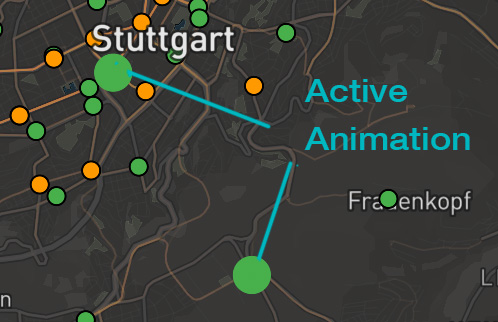
\includegraphics[width=0.34\textwidth]{vehicle_active.jpg}\label{fig:vehicle_active}}
      \hfill
      \subfloat[Vehicle beendet seinen Trip innerhalb von 30 Sekunden und wird inaktiv]{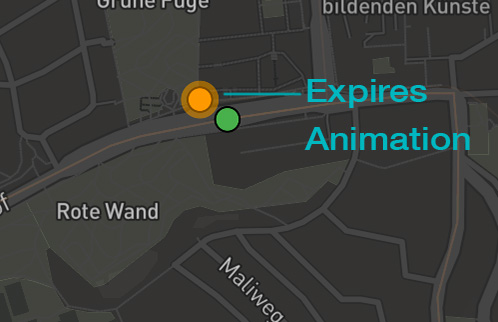
\includegraphics[width=0.34\textwidth]{vehicle_expires.jpg}\label{fig:vehicle_expires}}
      \caption{Vehicle Status Anzeige}
      \label{fig:vehicle_states}
    \end{figure}

    
    Ist ein Vehicle dabei, seinen Trip innerhalb von 30 Sekunden zu beenden, so wird ein leicht transparentes Pulsieren angezeigt. Nachdem das Vehicle den Trip beendet hat, wird es von der Karte genommen und verschwindet. Technisch betrachtet, werden erst alle Referenzen auf das Vehicle beseitigt und anschließend das Vehicle-Objekt gelöscht.
    
  % subsubsection vehicle (end)

  \subsubsection*{Zeitstrahl}
  \label{ssub:zeitstrahl}
    Die Webanwendung besitzt einen interaktiven Zeitstrahl am unteren Bildrand. Wie in Abbildung \ref{fig:timeline} zu sehen, besteht der Zeitstrahl aus mehreren Einzelteilen. 

    \begin{figure}[htbp]
      \begin{center}
        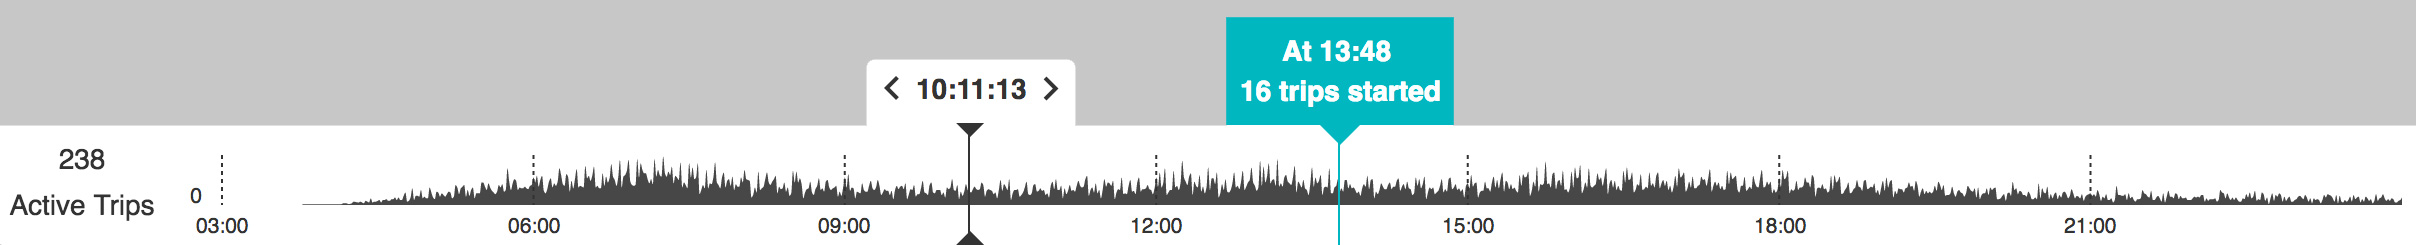
\includegraphics[width=\textwidth]{timeline}
        \caption{Zeitstrahl Komponente}
        \label{fig:timeline}
      \end{center}
    \end{figure}

    Links unten ist die Anzahl an momentan aktiven Trips zu sehen. Diese Anzahl korreliert mit den Vehicles auf der Karte. Die Anzeige wird immer aktuell gehalten und steigt, falls neue Trips aktiv werden, oder fällt wenn ein Trip beendet ist. Der Zeitstrahl selbst zeigt die Anzahl an aktiv werdenden Trips pro Minute an. Bewegt der Anwender die Maus darüber, so bekommt er die genaue Trip-Anzahl zu einer Uhrzeit als Tooltip angezeigt. Ebenfalls ist es möglich, die Animation zu einem beliebigen Zeitpunkt anzuzeigen. Dafür kann der Anwender einfach auf die gewünschte Zeitmarke im Zeitstrahl klicken und die Animation aktualisiert sich. Damit lässt sich die Karte zu unterschiedlichen Tageszeiten untersuchen. Zuletzt ist auch die gewählte Uhrzeit auf dem Zeitstrahl zu sehen. Diese zeigt dem Anwender, welcher Zeitpunkt momentan auf der Karte angezeigt wird.
    
  % subsubsection zeitstrahl (end)

  \subsubsection*{Filter}
  \label{ssub:filter}
    Über ein ausklappbares Menü lassen sich verschiedene Filter auswählen. Dadurch kann der Anwender zum Beispiel alle Vehicle eines Typs oder einer Linie abrufen. Auch Kombinationen der \texttt{Filter Vehicles} und \texttt{Filter Lines} sind möglich.

    Damit der Anwender die Relation zwischen Filter und Vehicles auf der Karte versteht, sind die Farben einheitlich gestaltet. Nachdem ein Filter ausgewählt ist, kann das Menü entweder wieder zugeklappt oder der Filter abgewählt werden.

    \begin{figure}[htbp]
      \begin{center}
        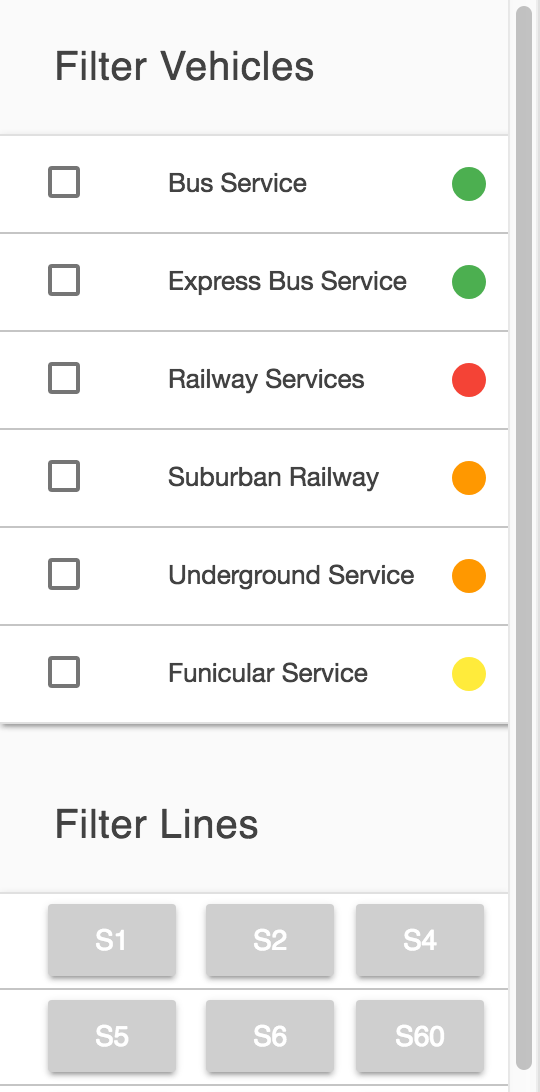
\includegraphics[width=0.2\textwidth]{filter}
        \caption{Filter Funktion}
        \label{fig:filter}
      \end{center}
    \end{figure}
    
  % subsubsection filter (end)

  \subsubsection*{Anzeigen von Trip Informationen}
  \label{ssub:anzeigen_von_trip_informationen}
    Wenn der Anwender ein Vehicle in der Karte durch Klicken auswählt, öffnet sich ein Fenster, welches Informationen für diesen Trip anzeigt (Abbildung \ref{fig:trip_information}. Neben dem Namen der Route lässt sich im Kreis (hier in Rot) die Routennummer ablesen. Im unteren Bereich sind die Fahrplaninformationen für den Trip gelistet. Neben dem Namen der Station ist auch die Abfahrtzeit des Vehicles gelistet. Die bereits besuchten Stationen werden in einem Grauton dargestellt, um sie als inaktiv zu markieren.

    \begin{figure}[htbp]
      \begin{center}
        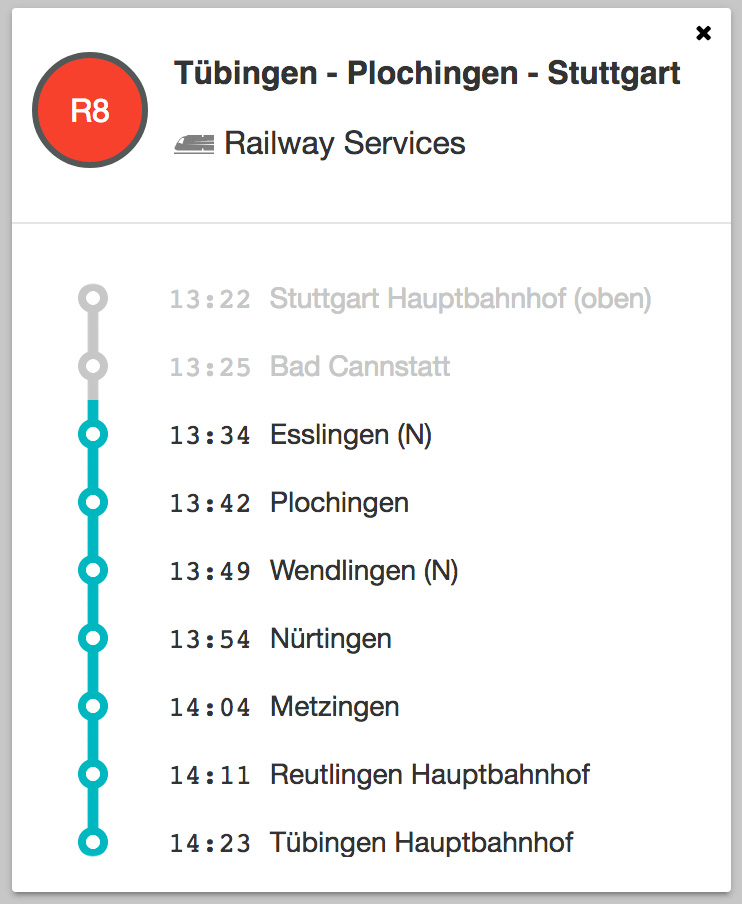
\includegraphics[width=0.3\textwidth]{trip_information}
        \caption{Anzeigen von Trip Informationen}
        \label{fig:trip_information}
      \end{center}
    \end{figure}
    
  % subsubsection anzeigen_von_trip_informationen (end)

  \subsubsection*{Wechseln der Kartendarstellung}
  \label{ssub:style_auswahl}
    Über das \texttt{Switch Style} Element {\Large \inlinegraphics{switch_styles_symbol}} hat der Anwender die Möglichkeit, zwischen verschiedenen Darstellungsarten der Karte zu wechseln. Auch die Polylines der Routen lassen sich zusätzlich über das Anwählen von \texttt{Shape} ein- oder ausblenden. Standardmäßig ist \texttt{Dark} ausgewählt.

    \begin{figure}[htbp]
      \begin{center}
        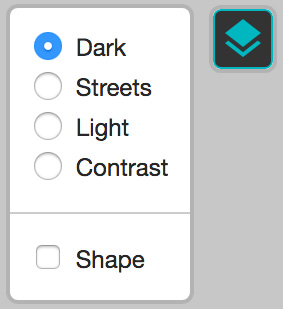
\includegraphics[width=0.14\textwidth]{switch_styles}
        \caption{Wechseln zwischen verschiedenen Kartendarstellung}
        \label{fig:switch_styles}
      \end{center}
    \end{figure}
    
  % subsubsection style_auswahl (end)

  \subsubsection*{Wegfindung}
  \label{ssub:wegfindung}
    Durch Klicken des \texttt{Line Finder} Buttons {\Large \inlinegraphics{line_finder_symbol}} lässt sich auf der Karte eine Route finden, die zwei Stationen $A, B$ verbindet. Dafür setzt der Anwender zwei Pins auf die Karte. Danach sucht ein Algorithmus diejenige Route aus, die am besten diese Stationen verbindet. Das Ergebnis sieht dann wie folgt aus:

    \begin{figure}[htbp]
      \begin{center}
        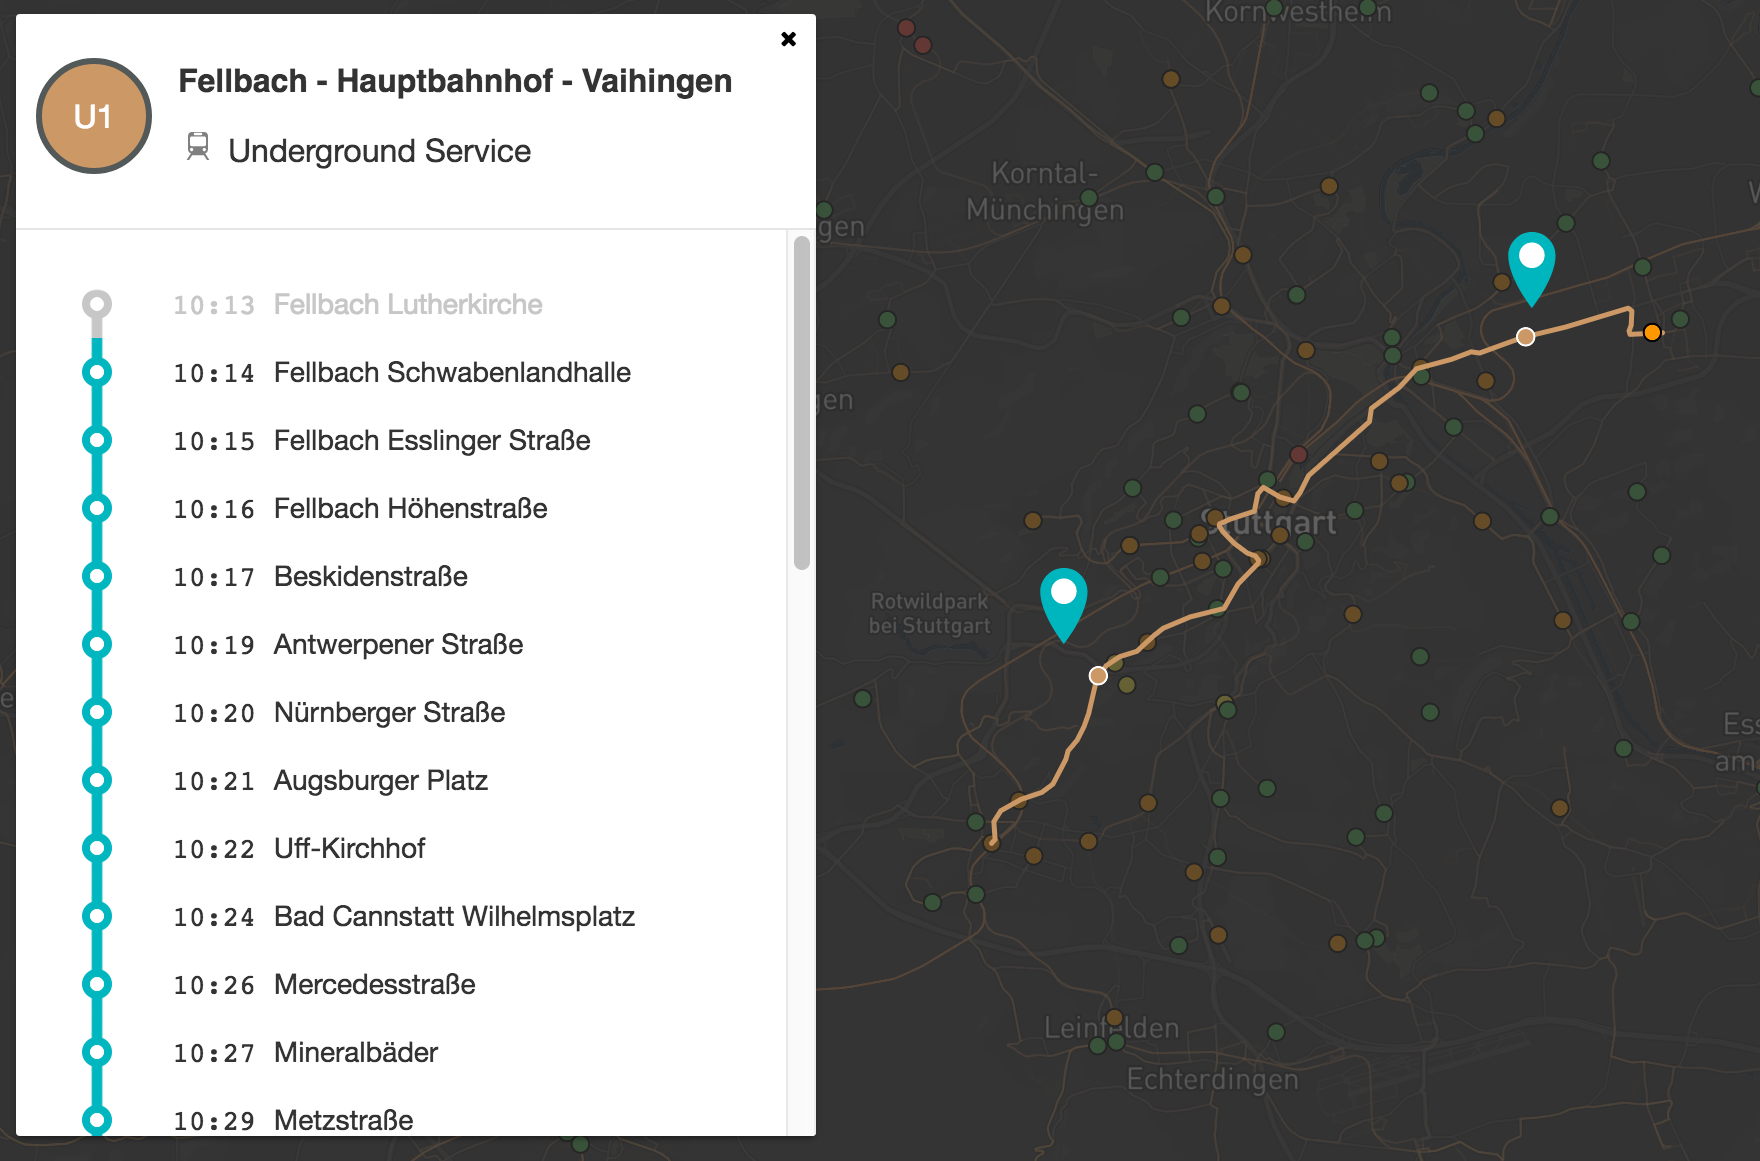
\includegraphics[width=0.6\textwidth]{line_finder}
        \caption{Linien Finder}
        \label{fig:line_finder}
      \end{center}
    \end{figure}

    Diese Funktion vereint Visualisierung und Wegfindung in einer Applikation. Während wir von anderen Applikationen gewohnt sind, eine Wegfindung ausschließlich über verschiedene Formularfelder (Von..., Nach..., Datum, Uhrzeit) anzufragen, könnte es für städtische oder regionale Wegfindung auch eine visuelle Lösung geben. Der Vorteil liegt dabei, dass kein Kontextwechsel nötig ist. Die Orientierung, Wegfindung und Fahrplaninformationen ließen sich alle in einer Ansicht vereinen. Ein weiteres Merkmal dieses visuellen Ansatzes ist die Möglichkeit, eine Route zu finden, ohne dass die Namen der Haltestellen bekannt sein müssen. Das auf der Karte dargestellte Ergebnis zeigt dem Nutzer auch sofort, wo sich das zur Route gehörende Vehicle momentan (oder zu einem bestimmten Zeitpunkt) befinden müsste. Damit könnte der Anwender auch gleich entscheiden, ob er dieses Vehicle noch erreichen würde oder nicht. Insbesondere an dieser Stelle wären GTFS-Realtime-Informationen von Nutzen, mit welchen beispielsweise Verspätungen mitangezeigt werden können.\\

    Von allen implementierten Komponenten bietet der Linien Finder das größte Potential für verschiedenste Weiterentwicklungen. Angefangen von der Implementierung von Echtzeitinformationen, über eine integrierte Anwender-Navigation (zum Beispiel könnte man den Anwender zu einer Station navigieren), bis zum Anbieten von Verbindungsanschlüssen bestünden Entwicklungsmöglichkeiten. Darüber hinaus kann der Algorithmus zur Auswahl der empfohlenen Route noch sehr viel weiter verbessert werden. Momentan fließt vor allem die mittlere Distanz zwischen gesetztem Pin und nächster Station in die Entscheidung ein. Weitere Faktoren könnten aber noch berücksichtigt werden. Beispielsweise der Typ des Vehicles (U-Bahn bevorzugt gegenüber Bus), Frequenz der Route, Wartezeit auf das Vehicle, Preis, Reisezeit oder gar das momentane Verkehrsaufkommen.
    
  % subsubsection linien_finder (end)
    
    % * Timeline Component (Time jump + Trip counter, Trips that get active)
    % * Vehicles, Vehicle States (active, inactive)
    % * Filtering mechanism (Lines / Type)
    % * Layer switcher
    % * Route finder
    % * Bezier Easing 
    
% subsection funktionen_der_webanwendung (end)
    
  % section deliver (end)
\end{newpage}

  \begin{newpage}
  \section{Fazit}
  \label{sec:fazit}
    In dieser Arbeit wurde aufgezeigt, wie durch die Verwendung von GTFS-Daten eine Live-Visualisierung des Öffentlichen Nahverkehrs für die Region Stuttgart erstellt werden konnte. Durch Technologien wie Mapbox, Nodjes und PostgreSQL wurde eine visuell ansprechende Anwendung entwickelt, die neben der Darstellung aktiver Fahrzeuge im zeitlichen Verlauf weitere Funktionen wie die einer visuellen Wegfindung bietet. Trotz hoher Datenmengen konnten die erwünschten Performance-Zielsetzungen erreicht werden. Der Mehrwert einer solchen interaktiven Karte ergibt sich vor allem für den verkehrsanalytischen Bereich. Hier kann die Karte zur überblicksartigen Erfassung des Verkehrsnetzes und dessen Analyse beitragen. Verkehrsdaten werden auf diese Weise also sowohl erfahr- als auch explorierbar gemacht.\\

    Für den gewöhnlichen Nutzer wäre der momentane Ansatz mit einer gesamten Abbildung des Öffentlichen Nahverkehrs einer Region allerdings auch mit Problemen behaftet. So ist die Übersichtlichkeit durch die Darstellung aller zu einem Zeitpunkt aktiven Fahrzeuge deutlich eingeschränkt und die Identifikation eines Fahrzeugs einer spezifischen Linie auf der Karte wird erschwert. Auch das Fehlen von GTFS-realtime in Stuttgart würde sich für ein konsumentenorientiertes Produkt nachteilig auswirken, da ohne Echtzeitkomponente viele Informationen, die für eine echte Live-Visualisierung wichtig wären, nicht angeboten werden können. Die Art der Anwendung suggeriert dem Nutzer zwar einen Ist-Zustand, da jedoch tatsächlich nur der Soll-Zustand übermittelt wird, bleiben Fahrplanänderungen oder -abweichungen unberücksichtigt.\\

    Als Ausblick für dieses Projekt wären diverse Verbesserungen möglich. Die Verknüpfung mit einer Echtzeitkomponente würde am meisten Potenzial für Weiterentwicklungen bieten. Die verschiedenen Stadien, die ein Fahrzeug annehmen kann (verspätet, verfrüht, pünktlich), könnten in die UI-Elemente mit einfließen und auch auf der Karte in kreativer Weise verarbeitet werden. Beispielsweise wären Änderungen in der farblichen Darstellung eines Vehicles je nach Pünktlichkeit oder Verspätung möglich. Aber auch statistische Auswertungen wie beispielsweise der Anteil an Verspätungen im Vergleich zum Vortag oder über einen gewissen Zeitraum (zu 34\% um 5 Minuten zu spät) könnten dem Anwender angezeigt werden. Möglich wäre auch, die "`Soll"'-Position, also wo sich das Fahrzeug laut Fahrplan eigentlich befinden sollte, im Vergleich zur tatsächlichen Position, anzuzeigen.

    Darüber hinaus könnte der "`Wegfinder"' aus Kapitel \ref{ssub:wegfindung} als Möglichkeit einer visuellen Wegfindung, Potenzial für Optimierungen und Raum für kreative neue Ideen in sich bergen. Hier könnten Tests mit echten Anwendern zeigen, inwieweit diese Möglichkeit anklang findet oder welche Änderungen für eine verbesserte Nutzbarkeit notwendig wären.

    Schlussendlich wurde aus dem Projekt noch die Erkenntnis gewonnen, dass Live-Karten im Allgemeinen wohl spezifischer auf die Anwendungsbereiche und Bedürfnisse entsprechender Nutzergruppen zugeschnitten sein müssten. Dies lässt sich aus der Zusammenschau der Vor- und Nachteile der in diesem Rahmen entwickelten Webanwendung, aber auch unter Berücksichtigung anderer bestehender Visualisierungen, schlussfolgern. Momentan gibt es zwar bereits verschiedene gute Produkte, die eine Live-Visualisierung des Öffentlichen Nahverkehrs - auch auf breiter Basis - abbilden, aber ich kenne niemanden in meinem Umfeld, der solch eine Anwendung verwendet. Dies kann zum einen daran liegen, dass all diese Anwendungen nicht primär für die native Nutzung per Smartphone - der Hauptnutzerbasis im Bereich Mobilität - entwickelt wurden, sondern eher auf Desktop oder Laptop-Bildschirmen gut darstellbar sind. Zum anderen benötigen unterschiedliche Usergruppen unterschiedliche Informationen. Ein Reisender beispielsweise ist im Zug auf andere Informationen angewiesen als ein Pendler. Ein Besucher in der Stadt findet sich anders zurecht als ein dort ansässiger Einheimischer. An einem öffentlichen Platz sind lokale, stationsbezogene Informationen am meisten relevant. Für Bahnstationen, aber auch für öffentliche Plätze oder gar Cafés, die nahe an einer Haltestelle liegen, könnte sich ein Live-Monitor nach Art von \url{http://transitscreen.com/live/} anbieten, welcher die nächstliegendsten Stationen und Linien anzeigt und dem Anwender umfassende Echtzeitinformationen rund um seinen Standort bietet. Deshalb wäre es bildlich gesprochen erfolgversprechender, anstatt einem großen Schweizer Taschenmesser, lieber viele kleinere Nieschenprodukte zu entwickeln. 

    Die im Rahmen dieser Masterarbeit entwickelte Live-Visualisierung stellt demgegenüber also eher ein Experten-Tool als eine Endanwender-Applikation dar. Allerdings könnte der entstandene Prototyp verwendet werden, um Evaluationen mit verschiedenen Endanwendern für eine nutzerspezifische Weiterentwicklung durchzuführen. Dadurch ließen sich eventuell neue spannende Erkenntnisse für die Entwicklung bisher unbekannter Produkte finden lassen.

  % section fazit (end)
\end{newpage}

  \begin{newpage}
\section{Anhang}
\label{sec:anhang}

\begin{lstlisting}[captionpos=t, caption=Postgresql Datenbankabfrage von allen aktiven Trips mit ihrem dazugehörigen Linienverlauf, label=lst:get_active_trips_query, language=SQL]
SELECT 
  array_to_json(ARRAY_AGG(array[stop_lat, stop_lon])) AS stops_coords,
  array_to_json(ARRAY_AGG(array[
    CAST ( stops.stop_id AS TEXT ),
    CAST ( stop_times.stop_sequence AS TEXT ),
    stops.stop_name, 
    stop_times.departure_time,
    CAST ( stop_times.departure_time_seconds AS TEXT ),
    stop_times.arrival_time,
    CAST ( stop_times.arrival_time_seconds AS TEXT )
  ] ORDER BY stop_times.stop_sequence)) AS stops_object,
  routes.route_short_name,
  routes.route_long_name,
  routes.route_type,
  routes.route_color,
  routes.route_text_color,
  trips.trip_id, 
  trips.route_id,
  trips.direction_id,
  frequency.start_time, 
  frequency.end_time, 
  frequency.start_time_seconds,
  frequency.end_time_seconds,
  frequency.headway_secs AS frequency_seconds,
  calendar.start_date,
  calendar.end_date,
  agencies.agency_timezone,
  agencies.agency_id,
  agencies.agency_name,
  array_to_json(ARRAY_AGG(array[shape_pt_lat, shape_pt_lon] 
    ORDER BY shape_pt_sequence ASC)) AS shape_coords
FROM gtfs_stop_times AS stop_times

INNER JOIN gtfs_trips AS trips
  ON trips.trip_id = stop_times.trip_id 
  AND trips.agency_key = stop_times.agency_key
    
INNER JOIN gtfs_routes AS routes
  ON routes.route_id = trips.route_id 
  AND routes.agency_key = trips.agency_key
   
INNER JOIN gtfs_agency AS agencies
  ON agencies.agency_id = routes.agency_id 
  AND agencies.agency_key = routes.agency_key

INNER JOIN gtfs_stops AS stops 
  ON stops.stop_id = stop_times.stop_id
  AND stops.agency_key = stop_times.agency_key
  AND NOT EXISTS (
    SELECT 0
    FROM denormalized_max_stop_sequence AS max
    WHERE max.agency_key = stop_times.agency_key
    AND max.trip_id = stop_times.trip_id
    AND max.trip_max = stop_times.stop_sequence
  )

LEFT JOIN gtfs_calendar_dates AS calendar_dates
  ON calendar_dates.service_id = trips.service_id
  AND calendar_dates.agency_key = trips.agency_key
  AND date = '2017-05-10' 
  AND calendar_dates.exception_type = 1

LEFT JOIN gtfs_calendar AS calendar 
  ON trips.service_id = calendar.service_id
  AND calendar.agency_key = trips.agency_key
  AND calendar.thursday = 1
  AND '2017-05-10' BETWEEN calendar.start_date 
  AND calendar.end_date OR calendar_dates.date IS NOT NULL
  AND calendar.start_date <= '2017-05-10'
  AND calendar.end_date >= '2017-05-10'

LEFT JOIN gtfs_frequencies AS frequency
  ON frequency.trip_id = trips.trip_id
  AND frequency.agency_key = trips.agency_key
    
LEFT JOIN gtfs_shapes AS shapes
  ON trips.shape_id = shapes.shape_id
  AND trips.agency_key = shapes.agency_key

WHERE (
  frequency.start_time_seconds >= 25200 
  AND frequency.end_time_seconds <= 90000
  AND shapes.shape_id IS NOT NULL
  AND '2017-05-10' BETWEEN calendar.start_date 
  AND calendar.end_date OR calendar_dates.date IS NOT NULL
) 
AND NOT EXISTS (
  SELECT 0
  FROM gtfs_calendar_dates AS date_exceptions
  WHERE date = '2017-05-10'
  AND date_exceptions.agency_key = trips.agency_key
  AND date_exceptions.service_id = trips.service_id
  AND exception_type = 2
)
GROUP BY 
  routes.route_short_name,
  routes.route_long_name,
  routes.route_type,
  routes.route_color,
  routes.route_text_color,
  trips.trip_id, 
  trips.route_id,
  trips.direction_id,
  frequency.start_time, 
  frequency.end_time, 
  frequency.start_time_seconds,
  frequency.end_time_seconds,
  frequency_seconds,
  calendar.start_date,
  calendar.end_date,
  agencies.agency_timezone,
  agencies.agency_id,
  agencies.agency_name
\end{lstlisting}


\begin{lstlisting}[captionpos=t, caption=Erstellen einer denormalized\_shapes Tabelle, label=lst:sql_aggregate_shape, language=SQL]
-- first we creat the new database table
CREATE TABLE denormalized_shapes (
  agency_key text,
  shape_id INTEGER,
  shape_coords json,
  shape_dist_traveled double precision[]
);

-- generating indexes
CREATE INDEX denormalized_shapes_unique_index 
  ON denormalized_shapes (agency_key, shape_id);

-- insert the shape data into new table
INSERT INTO denormalized_shapes
SELECT
  agency_key,
  shape_id,
  shape_coords,
  shape_dist_traveled
FROM (
  SELECT
    shapes.agency_key,
    shapes.shape_id,
    array_to_json(ARRAY_AGG(array[shape_pt_lon, shape_pt_lat]
      ORDER BY shape_pt_sequence ASC))
      AS shape_coords,
    ARRAY_AGG(shape_dist_traveled
      ORDER BY shape_pt_sequence ASC)
      AS shape_dist_traveled

  FROM gtfs_shapes AS shapes

  GROUP BY
    shapes.agency_key,
    shapes.shape_id
) as shp;
\end{lstlisting}

\begin{lstlisting}[captionpos=t, caption=Erstellen der denormalized\_shapes Tabelle, label=lst:denormalized_shapes, language=SQL]
-- create denormalized_trips table
CREATE TABLE denormalized_trips (
  stops_coords json NOT NULL,
  stops_object json NOT NULL,
  stops_dist_traveled json,
  agency_key TEXT NOT NULL,
  trip_id INTEGER NOT NULL,
  route_id INTEGER NOT NULL,
  service_id INTEGER NOT NULL,
  shape_id INTEGER,
  trip_start_time INTEGER NOT NULL,
  trip_end_time INTEGER NOT NULL,
  direction_id INTEGER,
  route_color TEXT,
  route_long_name TEXT,
  route_short_name TEXT,
  route_desc TEXT,
  route_type INTEGER
);
-- create indexes
CREATE INDEX denormalized_trips_index 
  ON denormalized_trips (agency_key, trip_id, route_id, shape_id);
-- now query the data and insert it into the newly created table
INSERT INTO denormalized_trips
SELECT
  stops_coords,
  stops_object,
  agency_key,
  trip_id,
  route_id,
  service_id,
  shape_id,
  trip_start_time,
  trip_end_time,
  route_color,
  route_long_name,
  route_short_name,
  route_desc,
  route_type
FROM (
  SELECT
    array_to_json(ARRAY_AGG(array[stop_lat, stop_lon]
      ORDER BY stop_times.stop_sequence::int)) AS stops_coords,
    array_to_json(ARRAY_AGG(array[
        stops.stop_id,
        CAST ( stop_times.stop_sequence AS TEXT ),
        stops.stop_name,
        stop_times.departure_time,
        CAST ( stop_times.departure_time_seconds AS TEXT ),
        stop_times.arrival_time,
        CAST ( stop_times.arrival_time_seconds AS TEXT )
    ] ORDER BY stop_times.stop_sequence::int)) AS stops_object,
    trips.agency_key,
    trips.trip_id,
    trips.route_id,
    trips.service_id,
    trips.shape_id,
    min(stop_times.arrival_time_seconds) as trip_start_time,
    max(stop_times.departure_time_seconds) as trip_end_time,
    routes.route_color,
    routes.route_long_name,
    routes.route_short_name,
    routes.route_desc,
    routes.route_type
  FROM gtfs_stop_times AS stop_times

  INNER JOIN gtfs_trips AS trips
    ON trips.trip_id = stop_times.trip_id
    AND trips.agency_key = stop_times.agency_key

  INNER JOIN gtfs_routes AS routes
    ON trips.agency_key = routes.agency_key
    AND routes.route_id = trips.route_id

  INNER JOIN gtfs_stops AS stops
    ON stops.stop_id = stop_times.stop_id
    AND stops.agency_key = stop_times.agency_key

  GROUP BY
    trips.agency_key,
    trips.trip_id,
    trips.route_id,
    trips.service_id,
    trips.shape_id,
    routes.route_color,
    routes.route_long_name,
    routes.route_short_name,
    routes.route_desc,
    routes.route_type
) as trps;
\end{lstlisting}

\begin{lstlisting}[captionpos=t, caption=Abfrage von Trips und dessen Polyline in einer Zeitspanne XY zu einem gegebenen Datum Z, label=lst:query_trips, language=SQL]
SELECT
  trips.stops_coords,
  trips.stops_object,
  trips.stops_dist_traveled,
  shapes.shape_coords,
  trips.route_id,
  trips.shape_id,
  trips.trip_id,
  trips.route_color,
  trips.route_desc,
  trips.route_type,
  trips.route_long_name,
  trips.route_short_name,
  trips.trip_start_time,
  trips.trip_end_time
FROM denormalized_trips AS trips

INNER JOIN gtfs_calendar_dates AS calendar_dates
ON calendar_dates.service_id = trips.service_id
AND calendar_dates.agency_key = trips.agency_key
AND date = 'YYYY-MM-DD'
AND exception_type = 1

-- GTFS STUTTGART-VVS does not make use of the calendar, 
-- if you want to process other feeds aswell you might need
-- to join this table too
--LEFT JOIN gtfs_calendar AS calendar
--  ON trips.service_id = calendar.service_id
--  AND calendar.agency_key = trips.agency_key
--  AND calendar.$date = 1

LEFT JOIN denormalized_shapes AS shapes
  ON trips.shape_id = shapes.shape_id
  AND trips.agency_key = shapes.agency_key

WHERE (
  trip_start_time BETWEEN XY AND XY
  AND shapes.shape_coords IS NOT NULL
)
--AND (
--  'YYYY-MM-DD' BETWEEN calendar.start_date AND calendar.end_date
--  OR calendar_dates.date IS NOT NULL
--)
AND NOT EXISTS (
  SELECT 0
  FROM gtfs_calendar_dates AS date_exceptions
  WHERE date = 'YYYY-MM-DD'
  AND date_exceptions.agency_key = trips.agency_key
  AND date_exceptions.service_id = trips.service_id
  AND exception_type = 2
)
\end{lstlisting}
  

\begin{lstlisting}[captionpos=t, caption=Geojson FeatureCollection als Antwort zu \texttt{/trips/:from,:to}, label=lst:geojson_featurecollection]
{
  2498: {
    "type": "FeatureCollection",
    "features": [24]
  },
  1925: {
    "type": "FeatureCollection",
    "features": [7]
  },
  ...
}
\end{lstlisting}


\begin{lstlisting}[captionpos=t, caption=Shape Feature, label=lst:shape_feature,texcl=true, language=JavaScript, literate={ö}{{\"o}}1]
"features": [
  {
    "type": "Feature",
    "properties": {
      "name": "shape",
      "route_color": "#FF0000",
      "route_type": 700,
      "trip_id": 8784,
      "route_short_name": "701",
      "route_long_name": "Sindelf. Eichholz - ZOB - Böbl. ZOB - Diezenhalde",
      "trip_start": 55560,
      "trip_end": 57780,
      "route_type_color": "#f44336",
      "polyline": "kswv@}x`jH_@f@}@?c@UiJ{AQHiBeAqDcCl@yAjAoB|@iAjBsC^cAOi@yCsA
      _FgAq@MuB@_@YkAa@}A]cDgAUM_FLoa@qBcHq@T{@eCqD_EoDoNiJoJwIaGuHaDqGaCmM?cF|
      @kFvLoSxDaFlG{EpAkA\mAFcBf@q@vA_CO_B[
      m@DiB^eANgAG}APuAbAeARYRm@HyA@}ISyBEiAKsGDsCf]aBmBgP]
      iDDiBNsAtBs@~GiBrAm@tCyEzCqCdDyB~FmC|AWhEY|R]
      rHAxKDnFAdMFvc@lE~JtA|Ex@bD`@vKrBnG~@nDRdBDfONj]z@jKlA`DNvC@zGS|E_@`Dg@zF
      sAxHqAlCa@rDKzIB|FLM\?f@|Fv@dBvC|@\d@s@H_CjCPjA@pKLHqBF_GD_@"
    },
    "geometry": {
      "type": "LineString",
      "coordinates": []
    }
  }
]  
\end{lstlisting}

\begin{lstlisting}[captionpos=t, caption=Station Feature, label=lst:station_feature]
{
  "type": "Feature",
  "properties": {
    "stop_id": "4637",
    "stop_sequence": 1,
    "stop_name": "Sindelf. Eichholz",
    "departure_time_secs": "55560",
    "arrival_time_secs": "55560",
    "secs_between_stops": 60,
    "dist_traveled": 0,
    "delta_dist_traveled": 0
  },
  "geometry": {
    "type": "Point",
    "coordinates": [
      9.002212,
      48.73068
    ]
  }
}
\end{lstlisting}

\begin{lstlisting}[captionpos=t, caption=Station Matching, label=lst:match_station, language=JavaScript]
const _ = require('lodash');
const knn = require('rbush-knn');
const rbush = require('rbush');
const turf = require('turf');

// own implementation of turf.js pointOnLine()
// https://github.com/Turfjs/turf/tree/master/packages/turf-point-on-line
function getPointOnLine(line, pt, units) {
  let coords;

  if (line.type === 'Feature') {
    coords = line.geometry.coordinates;
  } else if (line.type === 'LineString') {
    coords = line.coordinates;
  } else {
    throw new Error('input must be a LineString Feature or Geometry');
  }

  let closestPt = turf.point([Infinity, Infinity], { dist: Infinity });
  const start = turf.point(coords[0]);
  const stop = turf.point(coords[1]);
  start.properties.dist = turf.distance(pt, start, units);
  stop.properties.dist = turf.distance(pt, stop, units);
  // perpendicular
  const heightDistance = Math.max(start.properties.dist, stop.properties.dist);
  const direction = turf.bearing(start, stop);
  const perpendicularPt1 = turf.destination(pt, heightDistance, direction + 90, units);
  const perpendicularPt2 = turf.destination(pt, heightDistance, direction - 90, units);
  const intersect = turf.lineIntersect(
    turf.lineString([perpendicularPt1.geometry.coordinates, perpendicularPt2.geometry.coordinates]),
    turf.lineString([start.geometry.coordinates, stop.geometry.coordinates]));
  let intersectPt = turf.point([Infinity, Infinity], { dist: Infinity });
  if (intersect.features.length > 0) {
    intersectPt = intersect.features[0];
    intersectPt.properties.index = line.properties.index1;
    intersectPt.properties.dist = turf.distance(pt, intersectPt, units);
  }

  if (start.properties.dist < closestPt.properties.dist) {
    closestPt = start;
    closestPt.properties.index = line.properties.index1;
  }
  if (stop.properties.dist < closestPt.properties.dist) {
    closestPt = stop;
    closestPt.properties.index = line.properties.index2;
  }
  if (intersectPt && intersectPt.properties.dist < closestPt.properties.dist) {
    closestPt = intersectPt;
    closestPt.properties.index = line.properties.index1;
  }
  return closestPt;
}

// own implementation of turf.js pointOnLine()
// https://github.com/Turfjs/turf/tree/master/packages/turf-line-slice
function lineSlice(startPt, stopPt, line) {
  const start = turf.point(startPt, { index: 0 });
  let coords;
  if (line.type === 'Feature') {
    coords = line.geometry.coordinates;
  } else if (line.type === 'LineString') {
    coords = line.coordinates;
  } else {
    throw new Error('input must be a LineString Feature or Geometry');
  }
  const ends = [stopPt, start];
  const clipCoords = [ends[0].geometry.coordinates];
  for (let i = ends[0].properties.index + 1; i < ends[1].properties.index + 1; i += 1) {
    clipCoords.push(coords[i]);
  }
  clipCoords.push(ends[1].geometry.coordinates);
  return turf.lineString(clipCoords, line.properties);
}

function fillTree(trips) {
  const tree = rbush(200, ['[0]', '[1]', '[0]', '[1]', '[2]']);
  const coords = [];
  for (let k = 0; k < trips.features[0].geometry.coordinates.length; k += 1) {
    const item = [
      trips.features[0].geometry.coordinates[k][0],
      trips.features[0].geometry.coordinates[k][1],
      { index: k },
    ];
    coords.push(item);
  }
  tree.load(coords);
  return tree;
}

function matchStation(geojson) {
  _.forEach(geojson, (trips) => {
    const shape = _.first(trips.features);
    for (let i = 1; i < trips.features.length; i += 1) {
      const tree = fillTree(trips);
      const lat = trips.features[i].geometry.coordinates[0];
      const lng = trips.features[i].geometry.coordinates[1];
      const neighbours = knn(tree, lat, lng, 2);
      const line = turf.lineString([
        [neighbours[0][0], neighbours[0][1]],
        [neighbours[1][0], neighbours[1][1]]],
        { index1: neighbours[0][2].index, index2: neighbours[1][2].index });
      const pointOnLine = getPointOnLine(line, trips.features[i], 'kilometers');
      const lineDistance = turf.lineDistance(lineSlice(trips.features[0].geometry.coordinates[0], pointOnLine, shape));
      trips.features[i].properties.dist_traveled = lineDistance * 1000;
      trips.features[i].geometry.coordinates = pointOnLine.geometry.coordinates;

      if (i > 1) {
        const deltaDist = trips.features[i].properties.dist_traveled - trips.features[i - 1].properties.dist_traveled;
        trips.features[i].properties.delta_dist_traveled = Math.abs(deltaDist);
      } else {
        trips.features[i].properties.delta_dist_traveled = 0;
      }
    }
  });
  return geojson;
}

\end{lstlisting}

\end{newpage}
  \begin{newpage}
  \listoffigures
  \listoftables

  \renewcommand\lstlistlistingname{Listingverzeichnis}
  \lstlistoflistings
  \addcontentsline{toc}{section}{\lstlistlistingname}  
  
  \renewcommand*\listalgorithmname{Algorithmenverzeichnis}
  \listofalgorithms
  \addcontentsline{toc}{section}{\listalgorithmname}
   
  \printbibliography
  \addcontentsline{toc}{section}{Literatur}

\end{newpage}
  \begin{newpage}
	\thispagestyle{empty}
	% \hline
	\vspace*{\fill}
	\section*{Eidesstattliche Erklärung}
	Hiermit versichere ich, die vorliegende Arbeit selbstständig und unter ausschließlicher Verwendung der angegebenen Literatur und Hilfsmittel erstellt zu haben. Die Arbeit wurde bisher, in gleicher oder ähnlicher Form, keiner anderen Prüfungsbehörde vorgelegt und auch nicht veröffentlicht.\\

	\vspace{3cm}
	\begin{tabular*}{\textwidth}{c@{\extracolsep\fill}cc}
	\cline{1-1}
	\cline{3-3}
	\\
	\ \ \ \ \ \ \ \ \ Unterschrift \ \ \ \ \ \ \ \ \ \ & & \ \ \ \ \ \ \ \ \ Ort, Datum \ \ \ \ \ \ \ \ \ \\
	\end{tabular*}
\end{newpage}

\end{document}